\documentclass[a4paper,anonymous]{lipics-v2021}
%\documentclass[a4paper]{lipics-v2021}
%%% Options
% a4paper/letterpaper: for A4 paper format/for US-letter"
% UKenglish/USenglish: for british hyphenation rules/for american hyphenation rules
% numberwithinsect: for section-numbered lemmas etc.
% cleveref: for enabling cleveref support
% autoref: for enabling autoref support
% anonymous: for anonymousing the authors (e.g. for double-blind review)
% thm-restate: for enabling thm-restate support
% authorcolumns: for enabling a two-column layout for the author/affilation part (only applicable for > 6 authors)
% pdfa: for producing a PDF according the PDF/A standard

\pdfoutput=1 %uncomment to ensure pdflatex processing (mandatatory e.g. to submit to arXiv)
%\hideLIPIcs  %uncomment to remove references to LIPIcs series (logo, DOI, ...), e.g. when preparing a pre-final version to be uploaded to arXiv or another public repository

\bibliographystyle{plainurl}% the mandatory bibstyle

\title{Extending to Binders the Global Trace Condition for Cyclic Lambda-Calculus}
%\titlerunning{Extending to Binders the GTC for Cyclic $\lambda$-Calculus} %TODO optional, please use if title is longer than one line

\author
    {Stefano Berardi}
    {Computer Science Department, Turin University, Torino, Italy}
    {} % (Optional) email address
    {0000-0001-5427-0020} % (Optional) orcid
    {} % (Optional) author-specific funding acknowledgements

\author
    {Ugo de' Liguoro}
    {Computer Science Department, Turin University, Torino, Italy}
    {} % (Optional) email address
    {} % (Optional) orcid
    {} % (Optional) author-specific funding acknowledgements

\author
    {Daisuke Kimura}
    {Department of Information Science, Toho University, Japan}
    {} % (Optional) email address
    {} % (Optional) orcid
    {} % (Optional) author-specific funding acknowledgements

\author
    {Koji Nakazawa}
    {Graduate School of Informatics, Nagoya University, Japan}
    {} % (Optional) email address
    {} % (Optional) orcid
    {} % (Optional) author-specific funding acknowledgements

\author
    {Makoto Tatsuta}
    {National Institute of Informatics/Sokendai, Tokyo, Japan}
    {} % (Optional) email address
    {} % (Optional) orcid
    {} % (Optional) author-specific funding acknowledgements

    
\authorrunning{S.\,Berardi and U.\,de'\,Liguoro and D.\,Kimura and K.\,Nakazawa and M.\,Tatsuta}
% First: Use abbreviated first/middle names. Second (only in severe cases): Use first author plus 'et al.'

\Copyright{Stefano\,Berardi and Ugo\,de'\,Liguoro and Daisuke\,Kimura and Koji\,Nakazawa and Makoto\,Tatsuta}
% Please use full first names. LIPIcs license is "CC-BY";  http://creativecommons.org/licenses/by/3.0/

\ccsdesc[100]{Theory of computation}
% Please choose ACM 2012 classifications from https://dl.acm.org/ccs/ccs_flat.cfm 

\keywords{Cyclic proofs, Cyclic terms, Fixed-point definition, global trace condition, Lambda calculus, Infinitary lambda calculus}

\category{} %optional, e.g. invited paper

\relatedversion{} %optional, e.g. full version hosted on arXiv, HAL, or other respository/website
%\relatedversiondetails[linktext={opt. text shown instead of the URL}, cite=DBLP:books/mk/GrayR93]{Classification (e.g. Full Version, Extended Version, Previous Version}{URL to related version} %linktext and cite are optional

%\supplement{} %optional, e.g. related research data, source code, ... hosted on a repository like zenodo, figshare, GitHub, ...
%\supplementdetails[linktext={opt. text shown instead of the URL}, cite=DBLP:books/mk/GrayR93, subcategory={Description, Subcategory}, swhid={Software Heritage Identifier}]{General Classification (e.g. Software, Dataset, Model, ...)}{URL to related version} %linktext, cite, and subcategory are optional

%\funding{(Optional) general funding statement \dots}%optional, to capture a funding statement, which applies to all authors. Please enter author specific funding statements as fifth argument of the \author macro.

\acknowledgements{We thank Prof. Anupam Das for a valuable scientific correspondence about global trace condition for cyclic terms.} %optional

%\nolinenumbers %uncomment to disable line numbering

%Editor-only macros:: begin (do not touch as author)%%%%%%%%%%%%%%%%%%%%%%%%%%%%%%%%%%
\EventEditors{John Q. Open and Joan R. Access}
\EventNoEds{2}
\EventLongTitle{42nd Conference on Very Important Topics (CVIT 2016)}
\EventShortTitle{CVIT 2016}
\EventAcronym{CVIT}
\EventYear{2016}
\EventDate{December 24--27, 2016}
\EventLocation{Little Whinging, United Kingdom}
\EventLogo{}
\SeriesVolume{42}
\ArticleNo{23}
%%%%%%%%%%%%%%%%%%%%%%%%%%%%%%%%%%%%%%%%%%%%%%%%%%%%%%


%%%%%%%%%%%%%%%%%%%%%%%
%%%%%%%MY PACKAGES
%%%%%%%%%%%%%%%%%%%%%%%
\usepackage{graphicx}
\usepackage[all]{xy}
\usepackage{amssymb,amsmath,graphicx,color}
\usepackage{mymath,proof,latexsym}
\usepackage{xcolor}
\usepackage[pdftex,outline]{contour}
\usepackage{bussproofs}
\usepackage{tikz} % Tikz is required to use proofzilla
\usetikzlibrary{arrows.meta} % additional arrow styles
\usepackage{proofzilla}
%% PROOFZILLA SETTINGS %%%%%%%%%%%
% Flow-related macros 
% Define node style 
\newemptyvertex{node}{}
% Define edge styles: directed/undirected, color, arrow head etc
\defedgetype{flow}{draw=blue}{}
\defedgetype{dirflow}{-Latex,draw=blue}{}
\defedgetype{flowtwo}{draw=red}{}
\defedgetype{dirflowtwo}{-Latex,draw=red}{}
%%%%% HERE CHANGE THE DEFINITION OF EDGES TO CHANGE THE COLOR  AND OTHER ATRIBUTES %%%%%%
\defedgetype{dirflowblue}{-Latex,draw=blue}{}
\defedgetype{dirflowred}{-Latex,draw=red}{}
\definecolor{black}{gray}{0}
\defedgetype{flowblack}{-Latex,draw=black}{}
% Additional, unnecessary macros (terms etc)
%
%%%%%%%% COLORS and COMMENTS %%%%%%


\newcommand{\red}[1]{{\color{red} {#1}}}
\newcommand{\blue}[1]{{\color{blue} {#1}}}
\newcommand{\brown}[1]{{\color{brown} {#1}}}
\definecolor{ForestGreen}{RGB}{34,139,34}
\newcommand{\green}[1]{{\color{ForestGreen} {#1}}}
\newcommand{\black}[1]{{\color{black} {#1}}}
\newcommand{\purple}[1]{{\color{purple} {#1}}}
\newcommand{\orange}[1]{{\color{orange} {#1}}}

%\newcommand{\blue}[1]{{ \color{blue}{#1}}}
\newcommand{\pink}[1]{{\color{magenta}{#1}}}
\newcommand{\violet}[1]{{\color{violet}{#1}}}
\newcommand{\gray}[1]{{\color{gray}{#1}}}
\newcommand{\cyan}[1]{{\color{cyan}{#1}}}



%%%% GENERAL

\newcommand{\ie}{\textit{i.e.}\xspace}
\newcommand{\eg}{\textit{e.g.}\xspace}
\newcommand{\ih}{\textit{i.h.}\xspace}
\newcommand{\cf}{\textit{cf.}\xspace}

\newcommand{\rv}{r.v.\xspace}
\newcommand{\rvs}{r.v.s\xspace}
\newcommand{\cpt}{CPT\xspace}
\newcommand{\cpts}{CPTs\xspace}
\newcommand{\BN}{Bayesian network\xspace}
\newcommand{\BNs}{Bayesian networks\xspace}

\newcommand{\name}{name\xspace}
\newcommand{\names}{names\xspace}

\newcommand{\pax}{probabilistic axiom\xspace}
\newcommand{\paxs}{probabilistic axioms\xspace}

\newcommand{\linear}{low-level\xspace}
\newcommand{\basic}{\linear}
\newcommand{\exponential}{multiset\xspace}

%%
\newcommand{\defeq}{\triangleq}

%\newcommand{\grameq}{::=}
%\newcommand{\grammarpipe}{\mathrel{\big |}}
%\newcommand{\gpipe}{\grammarpipe}

\newcommand{\eqalpha}{\equiv_\alpha}


%%%%%%%%%  BAYESIAN NETWORKS, FACTORS

\newcommand{\Pa}[1]{\mathsf{Pa}(#1)}

\newcommand{\Val}[1]{\mathsf{Val}(#1)} %set of values of the RV #1

\newcommand{\Proj}[3][]{#2\vert_{#3}^{#1}} %projection of a value #2 of a set of rv #1 to a subset of rv #3 

\newcommand{\bn}{\mathcal{B}}
\newcommand{\FProd}{\odot} %product of factor (corresponding to tensor product + some diagonalisations), infix notation
\newcommand{\Fprod}{\FProd}
\newcommand{\BigFProd}{\bigodot} %n-ary product of factor (corresponding to tensor product + some diagonalisations)

\newcommand{\x}{\mathtt{x}}
\newcommand{\y}{\mathtt{y}}
\newcommand{\z}{\mathtt {z}}
\newcommand{\w}{\mathtt {w}}

\newcommand{\xs}{{\overline \x}}
\newcommand{\ys}{{\overline \y}}
\newcommand{\zs}{{\overline \z}}
\newcommand{\ws}{{\overline \w}}


%%% NAMES

\newcommand{\Names}{\textsf{Names}}

\newcommand{\XX}{\mathcal{X}}
\newcommand{\YY}{\mathcal{Y}}
\newcommand{\ZZ}{\mathcal{Z}}

\newcommand{\nX}{\mathsf{X}}
\newcommand{\nY}{\mathsf{Y}}
\newcommand{\nZ}{\mathsf{Z}}
\newcommand{\nW}{\mathsf{W}}
\newcommand{\nD}{\mathsf{D}}
\newcommand{\nS}{\mathsf{S}}
\newcommand{\nR}{\mathsf{R}}
\newcommand{\nO}{\mathsf{O}}
\newcommand{\nB}{\mathsf{B}}
\newcommand{\nU}{\mathsf{U}}

%\newcommand{\X}{\nX}
%\newcommand{\Y}{\nY}
%\newcommand{\Z}{\nZ}
%\newcommand{\W}{\nW}
%\newcommand{\D}{\nD}
%\newcommand{\R}{\nR}

\newcommand{\Xb}{\nX^{\bv}}
\newcommand{\Xt}{\nX^{\true}}
\newcommand{\Xf}{\nX^{\false}}
\newcommand{\Yb}{\nY^{\bv}}
\newcommand{\Yt}{\nY^{\true}}
\newcommand{\Yf}{\nY^{\false}}

\newcommand{\bX}{\mathbb X}
\newcommand{\bY}{\mathbb Y}
\newcommand{\bZ}{\mathbb Z}
\newcommand{\bS}{\mathbb S}
\newcommand{\bE}{\mathbb E}
\newcommand{\bC}{\mathbb C}
\newcommand{\bW}{\mathbb W}
\newcommand{\bJ}{\mathbb J}


\newcommand{\Nm}[1]{\mathsf{Nm}(#1)}
\newcommand{\ObsNm}[1]{\mathsf{ObsNm}(#1)}
\newcommand{\MainNm}[1]{\mathsf{MainNm}(#1)}
\newcommand{\PrivateNm}[1]{\mathsf{PrivateNm}(#1)}
\newcommand{\PublicNm}[1]{\mathsf{PublicMainNm}(#1)}

% Examples
\newcommand{\Dry}{\textsf{Dry}}
\newcommand{\Rain}{\textsf{Rain}}
\newcommand{\Sprinkler}{\textsf{Sprinkler}}
\newcommand{\Wet}{\textsf{Wet}}
\newcommand{\Broken}{\textsf{B}}
\newcommand{\User}{\textsf{U}}


%%%%%%%  TYPES %%%%%%%%%%%%

\newcommand{\iP}{P}
\newcommand{\iQ}{Q}
\newcommand{\iL}{L}
\newcommand{\iK}{K}
\newcommand{\iF}{F}

\newcommand{\iZero}{\bar{0}}
\newcommand{\iOne}{\bar{1}}
\newcommand{\iTwo}{\bar{2}}


\newcommand{\larrow}{\multimap}

\newcommand{\One}{\mathsf{1}} %unit tensor
\newcommand{\Zero}{\mathsf{0}} 
%\newcommand{\Bottom}{\mathsf \perp} 

\newcommand{\Real}{\mathbb{R}}
\newcommand{\Nat}{\mathbb{N}}
\newcommand{\bool}{\mathbf{B}}
\newcommand{\Bool}{\bool}


%%%% TERMS

%\newcommand{\Bang}{\lambda^{\oc}_{\text{\tiny\textsf{BN}}}}
\newcommand{\Bang}{\lambda^{\oc}_{\scriptscriptstyle\mathsf{BN}}}
\newcommand{\low}{\mathsf{low}}
\newcommand{\Low}{\lambda^{\scriptscriptstyle\mathsf{low}}_{\scriptscriptstyle\mathsf{BN}}}

\newcommand{\tm}{t}
\newcommand{\tmtwo}{u}
\newcommand{\tmthree}{r}

\newcommand{\tmu}{u}
\newcommand{\tmr}{r}
\newcommand{\tms}{s}

\newcommand{\var}{x}
\newcommand{\vartwo}{y}
\newcommand{\varthree}{z}
\newcommand{\vars}{\overline{x}}

\newcommand{\val}{v}
\newcommand{\valtwo}{w}

\newcommand{\true}{\mathtt{t}}
\newcommand{\false}{\mathtt{f}}
\newcommand{\bv}{\mathtt {b}}
\newcommand{\bvs}{\mathtt{\overline {b}}}

\newcommand{\prob}{p}
\newcommand{\dist}{d}
\newcommand{\sample}[1]{\mathtt{sample} \ {#1}}
\newcommand{\Bernoulli}[1]{\mathit{Bernoulli}_{#1}}
\newcommand{\coin}[1]{\mathtt{brn}_{#1}}

\newcommand{\der}{\mathtt{der}\; }

\newcommand{\observe}[2]{\mathtt{obs}(#1=#2)}
\newcommand{\obs}{\observe}
\newcommand{\obst}[1]{\observe{#1}{\true}}
\newcommand{\obsf}[1]{\observe{#1}{\false}}
\newcommand{\obsb}[1]{\observe{#1}{\bv}}

\newcommand{\pair}[2]{\langle #1, #2 \rangle}
\newcommand{\pattern}[1]{\langle #1 \rangle}

\newcommand{\letin}[3]{\mathtt{let} \; #1 = #2\; \mathtt{in} \; #3}
\newcommand{\letp}[3]{\mathtt{let} \; \pattern{#1} = #2 \; \mathtt{in} \; #3}
\newcommand{\leti}{\mathtt{let}\;}
\newcommand{\inl}{\;\mathtt{in}\;}

\newcommand{\tsc}{\mathbf{\mathtt{;}} \;} %semicolon separator

\newcommand{\caseSym}{\scalebox{0.8}[1]{ $ \Rightarrow $ }}
\newcommand{\case}[2]{\mathtt{case} \; #1 \; \mathtt{of} \; \{ #2 \} }

\newcommand{\ite}[3]{\mathtt{if} (#1, #2, #3)}
%\newcommand{\cons}[2]{#1\mathtt{::}#2}
\newcommand{\isZ}[1]{\mathtt{isZero} \; #1}
%\newcommand{\isE}[1]{\mathtt{isEmpty}(#1)}
%\newcommand{\head}[1]{\mathtt{head}(#1)}
%\newcommand{\tail}[1]{\mathtt{tail}(#1)}
\newcommand{\pred}[1]{\mathtt{pred} \; #1}
%\newcommand{\suc}[1]{\mathtt{succ}(#1)}
%\newcommand{\fix}[2]{\mathtt{fix}\;#1.#2}

\newcommand{\freevar}[1]{\langle #1 \rangle}
\newcommand{\CPT}[1]{\mathtt{cnd}_{\freevar{#1}}}
\newcommand{\CPTN}[2]{\mathtt{cnd}^{#1}_{\freevar{#2}}}

%Examples
\newcommand{\dry}{\textsf{dry}}
\newcommand{\rain}{\textsf{rain}}
\newcommand{\sprinkler}{\textsf{sprinkler}}
\newcommand{\wet}{\textsf{wet}}
\newcommand{\broken}{\textsf{broken}}
\newcommand{\user}{\textsf{user}}

\newcommand{\bias}{\textsf{bias}}
\newcommand{\ctoss}{\textsf{coin}}
\newcommand{\mycoin}{\CPT{\bias}}


%%%% NORMAL FORMS GRAMMAR

\newcommand{\gnf}{\mathsf{nf}}
\newcommand{\glv}{\mathsf{lv}}
\newcommand{\glp}{\mathsf{lp}}
\newcommand{\glx}{\mathsf{lx}}
\newcommand{\gprob}{\mathsf{pr}}

%%%% CONTEXTS

\newcommand{\hole}[1]{\llparenthesis #1 \rrparenthesis}
%\newcommand{\ctxhole}{\hole{\cdot}}

\newcommand{\cA}{\underline A}
\newcommand{\cB}{\underline B}
\newcommand{\cC}{\underline C}
\newcommand{\cP}{\underline P}
\newcommand{\cQ}{\underline Q}
\newcommand{\cI}{\underline I}
\newcommand{\cL}{\underline L}
\newcommand{\cK}{\underline K}
\newcommand{\cAp}[1]{\cA\hole{#1}}
\newcommand{\cPp}[1]{\cP\hole{#1}}
\newcommand{\cLp}[1]{\cL\hole{#1}}
\newcommand{\cKp}[1]{\cK\hole{#1}}
\newcommand{\cAnp}[2]{\cA_{#1}\hole{#2}}
\newcommand{\cPnp}[2]{\cP_{#1}\hole{#2}}
\newcommand{\cLnp}[2]{\cL_{#1}\hole{#2}}
\newcommand{\cKnp}[2]{\cK_{#1}\hole{#2}}
%\newcommand{\cLam}{\underline{\Lambda}}
\newcommand{\cLamnp}[2]{\underline{\Lambda}_{#1}\hole{#2}}
\newcommand{\cGamnp}[2]{\underline{\Gamma}_{#1}\hole{#2}}

% evaluation contexts
\newcommand{\evctx}{\mathsf{E}}

% substitution contexts
\newcommand{\sctx}{\mathsf{S}}
%\newcommand{\eslist}{\sctx}
\newcommand{\shole}[1]{\langle \mkern-5.5mu \langle #1 \rangle \mkern-5.5mu \rangle}
%\newcommand{\eshole}[1]{\shole{#1}}
%\newcommand{\sctxp}[1]{\sctx\holebag{#1}}
\newcommand{\sctxp}[1]{\sctx\shole{#1}}


%%%%%%  DERIVATIONS

\newcommand{\systemBN}{\mathscr{B}}
\newcommand{\systemBNb}{\mathscr{B}_{\oplus}}

\newcommand{\tjudg}[3]{#1\vdash #2:#3}

\newcommand{\demlow}{ \triangleright_\low }

% Rules
\newcommand{\isample}{\textsc{sample}\xspace}
\newcommand{\icond}{\textsc{cond}\xspace}
%\newcommand{\icoin}{\textsc{coin}\xspace}
\newcommand{\ipair}{\textsc{tuple}\xspace}
\newcommand{\ilet}{\textsc{let}\xspace}
\newcommand{\ivar}{\textsc{var}\xspace}
\newcommand{\iobs}{\textsc{obs}\xspace}
%\newcommand{\iletp}{\textsc{letp}\xspace}
\newcommand{\ibang}{\textsc{bang}\xspace}
\newcommand{\ider}{\textsc{der}\xspace}
\newcommand{\iapp}{\textsc{app}\xspace}
\newcommand{\iabs}{\textsc{abs}\xspace}
\newcommand{\iite}{\textsc{ite}\xspace}
\newcommand{\iitet}{\textsc{itet}\xspace}
\newcommand{\iitef}{\textsc{itef}\xspace}
\newcommand{\iitex}{\textsc{itex}\xspace}

\newcommand{\ovdash}[1]{\overset{\violet{#1}}{\vdash}}


%%%%%%% SEMANTICS

\newcommand{\Cpts}[1]{\mathsf{Cpts}(#1)}

\newcommand{\sem}[1]{\llbracket {#1} \rrbracket}
\newcommand{\den}[1]{{\sem{#1}}^\bullet}

\newcommand{\ft}[2]{ \overset{#2}{#1} }
\newcommand{\dmd}[1]{\, {\color{blue} \, \diamond \, #1} }
\newcommand{\dft}[2]{\, {\color{blue} \, \diamond \, \overset{#2}{#1}} }
\newcommand{\ftone}{ \mathbf{1} }

\newcommand{\dmdC}[1]{ {\color{violet} \, \diamond \, \scriptstyle{#1}} }
\newcommand{\dftC}[2]{ {\color{violet} \, \diamond \, \scriptstyle{#2}} }


%%%%%%% REDUCTION


%\newcommand{\isub}[2]{[#2 / #1]}
\newcommand{\esub}[2]{[#1=#2]}

\newcommand{\dB}{\mathsf{db}}
\newcommand{\dS}{\mathsf{dsub}}
\newcommand{\dbang}{\mathsf{der \oc}}
\newcommand{\dpair}{\mathsf{dpm}}  


\newcommand{\rrule}{\mathsf{r}}
\newcommand{\Root}[1]{\mapsto_{#1}}


%%%%%%%% FLOW %%%%%%%%

\newcommand{\Up}[1]{(#1)^-}
\newcommand{\Down}[1]{(#1)^+}
\newcommand{\up}[1]{{#1}^\uparrow}
\newcommand{\down}[1]{{#1}^\downarrow}


\newcommand{\flow}[1]{\mathsf{Flow}(#1)}
\newcommand{\Flows}[1]{\mathsf{Flows}(#1)}


%%%% SPECIFIC FROM SECTIONS

% evidence
\newcommand{\e}{\mathtt e}
\newcommand{\lessg}{\preceq}
\newcommand{\skeleton}[1]{\widehat{#1}} 

% cost 
\newcommand{\Npaxs}[1]{\mathsf{Npaxs}(#1)}
\newcommand{\BigO}[1]{\mathcal{O}(#1)}
\newcommand{\Exp}[1]{\mathsf{exp}(#1)}

% Beyond BN
\newcommand{\nsub}[2]{ {[#2/ #1]} }
\newcommand{\BigFMerge}[2]{\mathsf{Merge}_{#1}(#2)}
\newcommand{\FMerge}[1]{\underset{\scriptsize #1}{\bowtie}}
\newcommand{\ftr}{\mathbf{r}}

% Subj reduction
\newcommand{\tlet}{\mathtt{let}}


%%%%
\newcommand{\MaxNest}[1]{\mathsf{Nest}(#1)}
\newcommand{\OutBoxes}[1]{\mathsf{OutBoxes}(#1)}
\newcommand{\BoxStruct}[1]{\mathsf{BoxStruct}(#1)}
 
  
%% END PROOFZILLA SETTINGS %%%%%%%%%%%

\begin{document}

\maketitle

\begin{abstract}
Circular syntaxes for infinitary lambda-terms
were considered for instance by Ariola, Bl\"{o}m, Klop, Kennaway, Sleep, de Vries.
They allow to interpret lambda-terms written in fixed-point style 
as recursive definitions of infinitary terms. 
%In this way, circular syntax provides an 
%interpretation for basic constructions of functional programs, 
%like the letrec or mu of Clemens Grabmayer, Jan Rochel.
A sufficient, decidable and quite broad condition for reducing such 
infinitary lambda-terms to a numeral can be obtained
by adapting the global trace condition (GTC) to simply typed 
circular lambda-terms with conditional operator. 
GTC was originally proposed by Brotherston and Simpson
as a correctness condition for infinitary proofs.
Several people, including Das, Kuperberg, Pinault, Pous,
proved that GTC implies normalization to a numeral:
this result holds for a wide set of reductions and for closed circular lambda-terms 
with the type N of natural numbers. 

These papers considered a proper subset of infinitary lambda-terms, those
obtained from variables and combinators using a possibly infinite number of application.
Namely, these papers consider no \emph{explicit} clauses for lambda-abstraction,
which is instead defined through combinators.
Our contribution is to add explicit clauses for lambda-abstraction
to the definition of GTC, and to check that 
the extended GTC retains the termination properties of the original GTC. 
%Namely, we prove that the extended GTC implies normalization to some numeral, 
%for all closed infinitary terms of type N and
%for all reductions sequences not reducing inside the 
%predecessor clause for the conditional operator.  
\end{abstract}


% cut note 2

\def\Expand{{\rm expand}}

% cut elim

\def\RCLKIDomega{{{\bf RCLKID}^\omega}}
\def\Ren{{\rm Ren}}
\def\Terms{{\rm Terms}}
\def\IE{{\rm IE}}
\def\Cut{{\rm Cut}}
\def\Rcut{{\rm Rcut}}

% cmcs

\def\Co{{\rm co}}
\def\Axiom{{\rm Axiom}}
\def\Wk{{\rm Wk}}
\def\Cut{{\rm Cut}}
\def\BS{{\rm BS}}
\def\Bit{{\rm Bit}}
\def\LK{{\rm LK}}
\def\Head{{\rm head}}
\def\Tail{{\rm tail}}

% intuitionistic

\def\Univ{{\rm Univ}}
\def\Left{{\rm Left}}
\def\Right{{\rm Right}}
\def\Set{{\rm set}}
\def\ES{{\rm ES}}
\def\PC{{\rm PC}}
\def\Fin{{\rm Fin}}
\def\CLJIDomega{{{\bf CLJID}^\omega}}
\def\CLJIDHA{{{\bf CLJID}^\omega+{\bf HA}}}
\def\LJIDHA{{{\bf LJID}+{\bf HA}}}
\def\LJID{{\bf LJID}}
\def\OP{{\rm OP}}
\def\Div{{\rm Div}}
\def\RP{{\rm RP}}
\def\MS{{\rm MS}}
\def\ET{{\rm ET}}
\def\LiftedTree{{\rm LiftedTree}}
\def\First{{\rm first}}
\def\Er{{\rm Er}}
\def\ER{{\rm ER}}
\def\Insert{{\rm insert}}
\def\ET{{\rm ET}}
\def\SInd{{\rm SInd}}
\def\Trans{{\rm Trans}}
\def\HA{{\bf HA}}
\def\DM{{\rm DM}}
\def\Ext{{\rm ext}}
\def\KB{{\rm KB}}
\def\DT{{\rm DT}}
\def\DS{{\rm DS}}
\def\Monoseq{{\rm Monoseq}}
\def\Eq{{\rm seq}}
\def\Last{{\rm last}}

% equivalence cyclic proofs

%\def\Uor{\displaystyle \mathop {\widetilde\bigvee}}
\def\Uor{\biguplus}
\def\CLKIDomega{{{\bf CLKID}^\omega}}
\def\CLKIDPA{{{\bf CLKID}^\omega+{\bf PA}}}
\def\LKIDPA{{{\bf LKID}+{\bf PA}}}
\def\PA{{\bf PA}}

% simple equiv note

\def\LKIDN{{\bf LKIDN}}
\def\CLKIDN{{\bf CLKIDN}}

% equiv note

\def\Choose{{\rm Choose}}
\def\Asym{{\rm Asym}}
\def\Peano{{\bf Peano}}
\def\Code#1{{\lceil{#1}\rceil}}
\def\Ineq{{\rm Ineq}}
\def\MonoPath{{\rm MonoPath}}
\def\BoundedPath{{\rm BoundedPath}}
\def\InfPath{{\rm InfPath}}
\def\InfMonoPath{{\rm InfMonoPath}}
\def\HomSeq{{\rm HomSeq}}
\def\InfHomSeq{{\rm InfHomSeq}}

\def\ErdosTree{{\rm ErdosTree}}
\def\KB{{\rm KB}}
\def\MonoList{{\rm MonoList}}
%\def\Seq{{\rm Seq}}
\def\Univ{{\rm univ}}
\def\Infinite{{\rm Infinite}}
\def\S{{\bf S}}
%\def \N {{N}} %\def\N{{\bf N}} %
\def\Ind{{\rm Ind}}
\def\LKID{{\bf LKID}}
\def\PA{{\bf PA}}
\def\LKIDExt{{\bf LKIDExt}}
\def\CLKID{{\bf CLKID^\omega}}

% LICS

\def\Over#1#2{\deduce{#2}{#1}}
\def\List{{\rm List}}
\def\ListX{{\rm ListX}}
\def\ListO{{\rm ListO}}
\def\ListE{{\rm ListE}}
\def\Nl{{\rm nl}}

% CSLID

\def\SLLID{{\rm SLID}}
\def\SLID{{\rm SLID}}
\def\CSLID{{\rm CSLID}}
\def\CSLIDomega{{{\rm CSLID}\omega}}
\def\Eclass{{\rm Eclass}}
\def\Eq{{\rm Eq}}
\def\Deq{{\rm Deq}}
\def\Satom{{\rm Satom}}
\def\Cells{{\rm Cells}}
\def\Roots{{\rm Roots}}
\def\Elim{{\rm Elim}}
% \def\Case#1{{\rm Case-$#1$}}
\def\Case{{\rm Case}}
\def\Unfold{{\rm Unfold}}
\def\Pred{{\rm Pred}}
\def\Start{{\rm Start}}
\def\Unsat{{\rm Unsat}}
\def\Split{{\rm Split}}
\def\Underscore{\underline{\phantom{x}}}
\def\Rootcell{{\rm rootcell}}
\def\Rootshape{{\rm rootshape}}
\def\Jointleaf{{\rm jointleaf}}
\def\Jointleafimplicit{{\rm jointleafimplicit}}
\def\Jointnode{{\rm jointnode}}
\def\Directjoint{{\rm directjoint}}

% cyclicnote2

\def\Range{{\rm Range}}
\def\Xstart{X_{{\rm start}}}
\def\kstart{k_{{\rm start}}}
\def\Leaves{{\rm Leaves}}
\def\PureDist{{\rm PureDist}}
\def\Pure{{\rm Pure}}
\def\Identity{{\rm Identity}}
\def\Subst{{\rm Subst}}

% weak establish

\def\Connected{{\rm Connected}}
\def\Eststablished{{\rm Eststablished}}
\def\Valued{{\rm Valued}}

% monadic new

\def\SLRDbtw{{\rm SLRD}_{btw}}
\def\BTW{{{\rm BTW}}}
\def\Loc{{{\rm Loc}}}
\def\Ne{{\ne}}
\def\Nil{{{\rm nil}}}
\def\eqDef{=_{{\rm def}}}
\def\Inf#1{{\infty_{#1}}}
\def\Stores{{\rm Stores}}
\def\SVars{{{\rm SVars}}}
\def\Val{{{\rm Val}}}
\def\MSO{{{\rm MSO}}}
\def\Sep{{{\rm Sep}}}
\def\Septwo{{{\rm SLMI}}}
\def\SLMI{{{\rm SLMI}}}
\def\Sepinf{{\rm Sep}\infty}
\def\THeaps{{\rm THeaps}}
\def\Root{{\rm Root}}
\def\TG{{\rm TGraph}}

% monadic

\def\Nil{{{\rm nil}}}
\def\eqDef{=_{{\rm def}}}
\def\Inf#1{{\infty_{#1}}}
\def\Stores{{\rm Stores}}
\def\SVars{{{\rm SVars}}}
\def\Val{{{\rm Val}}}
\def\MSO{{{\rm MSO}}}
\def\Sep{{{\rm sep}}}
\def\THeaps{{\rm THeaps}}
\def\Root{{\rm Root}}
\def\TG{{\rm TGraph}}

\def\Tilde{\widetilde}
\def\Bar{\overline}
\def\Lequiv{\Longleftrightarrow}
\def\Lto{\Longrightarrow}
\def\Lfrom{\Longleftarrow}
\def\Norm{{\rm Norm}}
\def\Noshare{{\rm Noshare}}
\def\Roots{{\rm Roots}}
\def\Forest{{\rm Forest}}
\def\Var{{\rm Var}}
\def\Range{{\rm Range}}
\def\Cell{{\rm Cell}}
%\def\Tree{{\rm Tree}}
\def\Switch{{\rm Switch}}
\def\All{{\rm All}}
\def\To{\leadsto}
\def\tree{{\rm tree}}
\def\Paths{{\rm Paths}}
\def\Finite{{\rm Finite}}
\def\Const{{\rm Const}}
\def\Leaf{{\rm Leaf}}
\def\LeastElem{{\rm LeastElem}}
\def\LeastIndex{{\rm LeastIndex}}
\def\WSnS{{{\rm WSnS}}}
\def\Expand{{{\rm Expand}}}

% previous

\long\def\J#1{} % skip
\def\T#1{\hbox{\color{green}{$\clubsuit #1$}}}
\def\W#1{\hbox{\color{Orange}{$\spadesuit #1$}}}

\def\Node{{{\rm Node}}}
\def\LL{{{\rm LL}}}
\def\DSN{{{\rm DSN}}}
\def\DCL{{{\rm DCL}}}
\def\LS{{{\rm LS}}}
\def\Ls{{{\rm ls}}}

\def\FPV{{{\rm FPV}}}
\def\Lfp{{{\rm lfp}}}
\def\IsHeap{{{\rm IsHeap}}}

\def\Equiv{\quad \equiv\quad }
\def\Null{{{\rm null}}}
\def\Emp{{{\rm emp}}}
\def\If{{{\rm if\ }}}
\def\Then{{{\rm \ then\ }}}
\def\Else{{{\rm \ else\ }}}
\def\While{{{\rm while\ }}}
\def\Do{{{\rm \ do\ }}}
\def\Cons{{{\rm cons}}}
\def\Dispose{{{\rm dispose}}}
\def\Vars{{{\rm Vars}}}
\def\Locs{{{\rm Locs}}}
\def\States{{{\rm States}}}
\def\Heaps{{{\rm Heaps}}}
\def\FV{{{\rm FV}}}
\def\True{{{\rm true}}}
\def\False{{{\rm false}}}
\def\Dom{{{\rm Dom}}}
\def\Abort{{{\rm abort}}}
\def\New{{{\rm New}}}
\def\W{{{\rm W}}}
\def\Pair{{{\rm Pair}}}
\def\Lh{{{\rm Lh}}}
\def\lh{{{\rm lh}}}
\def\Elem{{{\rm Elem}}}
\def\EEval{{{\rm EEval}}}
% \def\BEval{{{\rm BEval}}} % not used 
\def\PEval{{{\rm PEval}}}
\def\HEval{{{\rm HEval}}}
\def\EVal{{{\rm Eval}}}
\def\Domain{{{\rm Domain}}}
\def\Exec{{{\rm Exec}}}
\def\Store{{{\rm Store}}}
\def\Heap{{{\rm Heap}}}
\def\Storecode{{{\rm Storecode}}}
\def\Heapcode{{{\rm Heapcode}}}
\def\Lesslh{{{\rm Lesslh}}}
\def\Addseq{{{\rm Addseq}}}
\def\Separate{{{\rm Separate}}}
\def\Result{{{\rm Result}}}
\def\Lookup{{{\rm Lookup}}}
\def\ChangeStore{{{\rm ChangeStore}}}
\def\ChangeHeap{{{\rm ChangeHeap}}}
\def\Wand{\mathbin{\hbox{\hbox{---}$*$}}}
%\def\Eval#1{[\kern -1pt[{#1}]\kern -1pt]}
\def\Eval#1{\llbracket{#1}\rrbracket}
\def\Vec{\overrightarrow}

\def\Tilde{\widetilde}
\def\Break{\hfil\break\hbox{}}

%Macro for the work on Cyclic System T with lambda
%22/03/2024
\newcommand{\ap}                { {\tt ap} }
\newcommand{\cond}            { {\tt cond} }
\newcommand{\mapsfrom} {\mathbin{\leftarrow\!\!\rule[0.3pt]{0.5pt}{4pt}\,}}
\newcommand{\reduces}       { \mathbin{\mapsto} }
\newcommand{\CTlambda}    { { {\tt CT}\mbox{-}\lambda} }
\newcommand{\CT}                { {\tt CT} }
%\newcommand{\nameIn}       { {\tt name\mbox{-}in} }
\newcommand{\etaRule}       { {\eta\mbox{-rule}} }
\newcommand{\ins}               { {\tt ins} }
\newcommand{\struct}          { {\tt struct} }
\newcommand{\Iter}              { {\tt It} }
\newcommand{\iter}               { {\tt it} }
\newcommand{\Interval}       { {\tt In} }
\newcommand{\interval}        { {\tt in} }
\newcommand{\Succ}             { {\tt S} }
\newcommand{\nil}                { {\tt nil} }
\newcommand{\cons}             { {\tt cons} }
\newcommand{\outline}  [1]   { {\contour{black}{\textcolor{white}{#1}}}  }
\newcommand{\systemT}       { {\outline{\tt T}} }
\newcommand{\LAMBDA}       { {\outline{$\Lambda$}} }
\newcommand{\Rec}               { {\tt Rec} }
\newcommand{\rec}                { {\tt rec} }
\newcommand{\exch}             { {\tt exch} }
\newcommand{\composed}     { {\mbox{\tiny $\circ$}} }
\newcommand{\WTyped}        { {\tt WTyped} }
\newcommand{\safe}              { {\hbox{\scriptsize \tt safe}} }
\newcommand{\GlobalTraceCondition}  { {\tt GlTrCon} }
\newcommand{\Sum}              { {\tt Sum} }
\newcommand{\safeReduces} {\mathbin{\reduces_\safe}}
\newcommand{\nsafeReduces}[1] {\mathbin{\reduces_{#1,\safe}}}
\newcommand{\nsafeReducesL}[1] {\mathbin{\mapsfrom_{#1,\safe}}}
\newcommand{\nsafeReducesAstL}[1] {\mathbin{\mapsfrom_{#1,\safe}^*}}
\newcommand{\safeReducesAst} {\mathbin{\reduces_\safe^*}}
\newcommand{\nsafeReducesAst}[1] {\mathbin{\reduces_{#1,\safe}^*}}
\newcommand{\nsafePReduces}[1] {\mathbin{\Rightarrow_{#1}}}
\newcommand{\nsafePReducesL}[1] {\mathbin{\Leftarrow_{#1}}}
\newcommand{\nsafePReducesMany}[2] {\mathbin{\Rightarrow_{#1}^{#2}}}
\newcommand{\nsafePReducesManyL}[2] {\mathbin{\Leftarrow_{#1}^{#2}}}
\newcommand{\nequal}[1] {\mathbin{\approx_{#1}}}
\newcommand{\var}                { {\tt var} }
\newcommand{\Graph}            { {\tt Graph} }
\newcommand{\bfColor} [2]     {{\bf \color{#1}{#2}}}
\newcommand{\weak}             {{\tt weak}}

%colors from the web site: https://latexcolor.com/
\definecolor{amber}{rgb}{1.0, 0.75, 0.0}
\definecolor{oldgold}{rgb}{0.81, 0.71, 0.23}

\newcommand{\SubTerm}               {{\tt SubT}}
\newcommand{\LSubTerm}[2]           {{\tt Sub_{#1}(#2)}}
\newcommand{\Lctx}[1]           {{\tt C}_{#1}}
\newcommand{\Lv}[2]           {||#2||_{#1}}
\newcommand{\Tree}                      {{\tt Tree}}
\newcommand{\N}                           {{N}}
\newcommand{\Num}                      {{\tt Num}}
\newcommand{\Nat}                        {{\outline{\tt N}}}
\newcommand{\GTC}                       {{\tt GTC}}
\newcommand{\Reg}                       {{\tt Reg}}
\newcommand{\Type}                      {{\tt Type}}
\newcommand{\conc}                      {{\star}}
\newcommand{\typingRule}            {{\tt r}}
%\newcommand{\apvar}                     {{\ap_{\mbox{\tiny var}}}}
%\newcommand{\apnotvar}               {{\ap_{\neg\mbox{\tiny var}}}}
\newcommand{\apvar}                    {{{\tt ap}_{\mbox{\tiny $v$}}}}
\newcommand{\apnotvar}               {{{\tt ap}_{\mbox{\tiny $\neg v$}}}}
\newcommand{\subseteqsim}         {\mathbin{\raisebox{2pt}{$\subset$}_{\!\!\!\!\!\sim}}}
\newcommand{\supseteqsim}         {\mathbin{\raisebox{2pt}{$\supset$}_{\!\!\!\!\!\sim}}}
\newcommand{\Ctxt}                       {{\tt Ctxt}}
\newcommand{\Seq}                        {{\tt Seq}}
\newcommand{\Stat}                       {{\tt Stat}}
\newcommand{\Rule}                       {{\tt Rule}}
\newcommand{\restr}                      {{\lceil}}
\newcommand{\setT}                       {{\mathcal T}}
\newcommand{\base}                      {{\tt base}}
\newcommand{\inductive}               {{\tt ind}}
\newcommand{\universe}     [1]       {{|#1|}}
\newcommand{\Label}                     {{\tt Lbl}}
\newcommand{\quotationMarks} [1]     {{\textquotedblleft#1\textquotedblright}}
\newcommand{\lexicographic} [1]   {{ <^{#1}_{\mbox{\tiny lex}}} }
\newcommand{\trunk}                     {{\tt trunk}}


\newcommand\Restrict[2]{#1_{#2}}
\newcommand\simIndex[1]{\sim^{#1}_{{\tt idx}}}
\newcommand\mergeCtx[2]{#1\sharp#2}
\newcommand\Ifz{{\tt ifz}}
\newcommand\TtoCT[1]{(#1)^\circ}


%\definecolor{oldgold}{rgb}{0.81, 0.71, 0.23}
\definecolor{purple}{rgb}{0.8, 0.2, 0.8}

\newcommand{\Rapv}{\hbox{$(\text{ap}_{\text{v}})$}}
\newcommand{\RapNv}{\hbox{$(\text{ap}_{\lnot\text{v}})$}}
\newcommand{\Reta}{\hbox{$(\eta)$}}
\newcommand{\Rap}{\hbox{$(\text{ap})$}}
\newcommand{\Rcond}{\hbox{$(\text{cond})$}}
%\newcommand{\FV}[1]{\text{FV}(#1)}
\newcommand{\Ack}{{\tt Ack}}
\newcommand{\AckA}{{\tt ack1}}
\newcommand{\AckB}{{\tt ack2}}
\newcommand{\ACK}{{\redM Ack}}
\newcommand{\Cond}[2]{{\tt cond}(#1,#2)}
\newcommand{\Suc}[1]{{\tt S}(#1)}
%\newcommand{\N}{N}
\newcommand{\goldN}{{\bfColor{oldgold}{N}}}
\newcommand{\redN}{{\bfColor{red}{N}}}
\newcommand{\bluen}{{\bfColor{blue}{n}}}
\newcommand{\redm}{{\bfColor{red}{m}}}
\newcommand{\blueN}{{\bfColor{blue}{N}}}
\newcommand{\redblueN}{{\bfColor{red}{N}\hspace{-1em}\bfColor{blue}{N}}}

%\newenvironment{claim}[1][Claim]{\begin{trivlist}\item[\hskip \labelsep {\bfseries #1}]}{\end{trivlist}}



\newcommand{\Pfin}                       {{\setP_{\mbox{\tiny fin}}}}
\newcommand{\eqMap}                  {{\tt eq}}
\newcommand{\BadSeq}                 {{\tt BadS}}


\newcommand{\labelled}                  { {\mbox{\tiny \tt lab}} }  
\newcommand{\CTlambdaLabelled} {{\mbox{\tt lab-}\CTlambda}}
\newcommand{\parallelReduces}         { {  \mapsto \mspace{-17mu} \mapsto  }}
%18 mu = 1 large character, like M
\newcommand{\length}                     {{\tt len}}
\newcommand{\form}                     {{\tt form}}
\def\head                                         {{\rm head}}   
                  


% Section 1
% !TEX root = main.tex

\section{Introduction}

We consider $\LAMBDA$, the set of infinitary simply typed $\lambda$-terms 
with conditional on zero, in the style for instance of 
Ariola, Bl\"{o}m, Klop, Kennaway, Sleep, de Vries 
(\cite{ARIOLA1997154,10.1007/BFb0014548,KENNAWAY199793}).

The types of $\LAMBDA$ are all simple types obtained from the atomic type $\N$
and type variables.
The terms of $\LAMBDA$  are all possibly infinite trees representing expressions 
defined with $0$, $\Succ $, $\ap$ (application), 
variables $x^T$ (with a type superscript $T$),  $\lambda$ (the binder for defining 
maps), and $\cond$, the arithmetic conditional (i.e., the test on zero, with predecessor included). 
We imagine that the infinite terms of $\LAMBDA$ describe
a simplified functional language with fixed point, like the functional language considered by
 Clemens Grabmayer, Jan Rochel (\cite{Letrec,Letmu,JanRochelPhd2016}).
As usual, we add reduction rules with the goal of transforming closed terms of type $\N$ 
into notations for natural numbers. Thus, 
the closed terms of $\LAMBDA$ can be interpreted as partial functionals on $\N$.
In the general case a reduction on a closed terms of type $\N$ can continue forever,
this is why without further conditions we only obtain partial functionals.

%19:42 19/04/2024

In this paper we will mainly consider regular terms, namely, possibly infinite $\lambda$-terms 
having a finite number of distinct subterms. This is the frame we work in.
We introduce a set of terms we call $\CTlambda$, consisting of all 
regular terms satisfying a condition called Global Trace Condition (GTC).
The definition of $\CTlambda$ and a termination  result for it is our contribution.


GTC has been introduced for infinitary proofs 
by J. Brotherston and A. Simpson
(\cite{BrotherstonPhd2006}, \cite{BrotherstonSimpson2011}), then adapted
to algebraic terms of G\"{o}del system $\systemT$ by Das, Kuperberg, Pinault, Pous 
(\cite{2021-Anupam-Das,DBLP:conf/fscd/000221,DBLP:conf/lics/Curzi022,DBLP:conf/csl/Curzi023,DBLP:conf/lics/Curzi023}).

Our contribution is to extend these circular versions of G\"{o}del system $\systemT$ 
(\cite{GoedelSystemT}) by adding an explicit use of the binder $\lambda$. Adding $\lambda$,  
we hope to provide a circular syntax more familiar to researchers working in the
field of Type Theory. % We call $\CTlambda$ our extended circular syntax.

We will prove for $\CTlambda$ (with binders) a result which was only
known for the \emph{algebraic} circular syntax for system $\systemT$:
that reductions not in the second argument of any $\cond$ (conditional)
strongly normalizes, and that they always reduce closed normal terms of type 
$\N$ to a numeral.

We also quote a second contribution. We extend to the case of binder $\lambda$ the
characterization of the limit reduction obtained 
by Das, Kuperberg, Pinault, Pous 
(\cite{2021-Anupam-Das,DBLP:conf/fscd/000221,DBLP:conf/lics/Curzi022,DBLP:conf/csl/Curzi023,DBLP:conf/lics/Curzi023})
for the algebraic circular version of 
G\"{o}del system $\systemT$. Namely, we prove that all infinite reductions on $\CTlambda$
have a limit, which informally can be described as follows. 
In each infinite reduction sequence
the first symbol of the $\lambda$-term eventually stabilizes, then the
first symbol of each immediate subterm eventually stabilizes, and so forth, recursively.

The notion of limit reduction in $\CTlambda$
could be considered similar to the notion of limit reduction for finite $\lambda$-terms obtained
through B\"{o}hm trees (\cite{Barendregt1984}, Def. 10.1.4). 
However, we stress that there is an important difference: 
in $\CTlambda$ no \quotationMarks{undefined} subterm is required
in order to represent the limit of a reduction, while B\"{o}hm trees 
can have undefined subtrees. 

This is the plan of the paper. In Section~\ref{section-infinite-lambda}, we introduce
the set $\LAMBDA$ of our infinite $\lambda$-calculus,
including its types, terms, typing rules, and reduction rules.
Section~\ref{section-trace-infinite-lambda-terms} and Section~\ref{section-circular-system-CTlambda}
introduce the notion of traces and the global trace condition for $\LAMBDA$, respectively.
Section~\ref{section-subject-reduction} mentions the subject reduction
for terms of $\LAMBDA$ with GTC. 
Section~\ref{section-finite-safe-reductions} introduces the notion of $n$-safe-reductions
that compute finite approximations of the limit normal forms of infinite reductions, 
and also shows that any closed $\CTlambda$ term of type $\N$ is reduced to a numeral
by reducing in any way with $0$-safe-reductions. 
Section~\ref{section-comparison} compares our work with some related work. 
Section~\ref{section-conclusion} concludes the current paper, mentioning our plan 
for further works. 


%14:57 17/04/2024
%21:08 19/04/2024




% Section 2
\section{The set of infinite $\lambda$-terms}
We define the set $\LAMBDA$ of infinite circular terms, the subset $\WTyped$
of well-typed terms and a reduction relation for them. They will be used to
give a semantics for finite circular notations for $\lambda$-terms.
Infinite terms are labeled binary trees, therefore we
recall what are binary trees first.
%, and before them the lists on $\{1,2\}$ and
%some related notions.
%
%\subsection{Lists and Binary Trees}
%
%\begin{definition}(Lists on $\{1,2\}$)
%\begin{enumerate}
%\item
%We denote with $\List(\{1,2\})$ the set of all lists on $\{1,2\}$, just lists for short.
%\item
%If $i_1, \ldots, i_n \in \{1,2\}$, we write $(i_1, \ldots, i_n)$
%for the list with elements $i_1, \ldots, i_n$. 
%\item
%We write $\nil$ for the empty list, or $()$. 
%\item
%If $l=(i_1, \ldots, i_n), m=(j_1, \ldots, j_m) $ are lists
%we define
%$
%l \conc m = (i_1, \ldots, i_n,\ j_1, \ldots, j_m)
%$
%%If $I \subseteq \List(\{1,2\})$
%%we write $l \conc I = \{l \conc m | m \in I\}$. 
%\item
%The prefix order $\le$ on lists
%is defined by $l \le m$ if and only if $m = l \conc m'$ for some $m' \in  \List(\{1,2\})$.
%\end{enumerate}
%\end{definition}

Binary trees are represented by sets of lists on $\{1,2\}$.

\begin{definition}(Binary trees)
\begin{enumerate}
\item 
A binary tree, just a tree for short, is any set $T\subseteq \List(\{1,2\})$ 
of lists including the empty list and closed by prefix: $\nil \in T$ and for all $l, m \in \List(\{1,2\})$
if $m \in T$ and $l \le m$ then $l \in T$. 
\item
$\nil$ is called the root of $T$, any $l \in T$ is called a node of
$T$ and if $l \in T$, then any $l \conc (i) \in T$ is called a child of $l$ in $T$
of index $i$.
\item
A node $l$ of $T$ is a leaf of $T$ if $l$ is an maximal element of $T$ w.r.t. the prefix order (i.e.,
if $l$ has no children). 
\item
If $T$ is a tree and $l \in T$ we define $T \restr l = \{m \in \List(\{1,2\}) | l \conc m \in T\}$.
$T \restr l$ is a tree and we say that $T \restr l$ is a subtree of $T$ in the node $l$,
and for each $m \in T \restr l$ we say that $l \conc m$ is the corresponding node in $T$.
\item
If $l=(i)$ we say that $T_l$ is an immediate sub-tree of $T$.
\item
A binary tree labeled on a set $L$ is any pair $\setT = (T, \phi)$ with 
$\phi:T \rightarrow L$. We call $\universe{\setT}=T$ the set of nodes of $\setT$.
For all $l \in T$ we call $\Label(\setT,l) = \phi(l)$ the label of $l$ in $\setT$.
\item
We define $\setT \restr l = (T \restr l, \phi_l)$ and $\phi_l(m) = l \conc m$. 
We call any $\setT \restr l$ a labeled subtree of $\setT$
in the node $l$, an immediate sub-tree if $l=(i)$. 
\end{enumerate}
\end{definition}

Remark that the labeling of a node $m \in \universe{( \setT \restr l )}$ 
is the same label of the corresponding node $l \conc m$ of $\universe{\setT}$.
 
Let $n = 0, 1, 2$. We define an operation $l(\setT_1, \ldots, \setT_n)$
combining labeled trees which we will use to produce tree notation. 
Assume $\setT_1, \ldots,\setT_n$ are trees labeled on $L$ and $l \in L$.
Then we define $$\setT = l(\setT_1, \ldots, \setT_n)$$ 
as the unique tree $\setT$ labeled on $L$ with the root labeled $l$ and with:
$\setT \restr (i) = \setT_i$ for all $1 \le i \le n$.


\subsection{Types, Terms and Contexts}
Now we define our semantics for circular $\lambda$-terms,
the set $\LAMBDA$ of infinite tree notations: first the types of $\LAMBDA$, 
then the terms and the contexts of $\LAMBDA$.

\begin{definition}(Types and Variables of $\LAMBDA$)
%\mbox{}
\begin{enumerate}

\item
The types of $\LAMBDA$ are: the type $\N$ of natural numbers, an infinite list 
$\alpha,\beta,\ldots$ of type variables, and with $A,B$ also  $A \rightarrow B$.
We call them simple types, just \emph{types} for short. 

\item 
$\Type$ is the set of simples types.

\item
We suppose be given a set $\var$, consisting of all pairs $x^T=(x,T)$ 
of a variable name $x$ and a type $T \in \Type$.
\end{enumerate}
\end{definition}

Terms of $\LAMBDA$ are possibly infinite binary trees, with each node labeled by 
some operation on $\lambda$-terms of arity $0,1,2$.


\begin{definition}(Terms of $\LAMBDA$)
The terms of $\LAMBDA$ 
are all binary trees $t$ with set of labels 
$L=\{x^T, \ \lambda x^T., \ \ap, 0, \ \Succ, \ \cond\}$ such that:
\begin{enumerate}
\item 
a node $l$ labeled $x^T$ or $0$ is a leaf of $t$ (\emph{no} children). 
\item
a node $l$ labeled $\lambda x^T.$ or $\Succ$ has a \emph{unique} 
child $l \conc (1)$. 
\item
a node labeled $\ap$, $\cond$ has \emph{two} children $l \conc (1)$, $l \conc (2)$.
\end{enumerate}
As usual, we abbreviate $\ap(t,u)$ with $t(u)$.

We say that $t$ is a sub-term of $u$ if $t$ is a labeled sub-tree of $u$,
an immediate subterm if it is an immediate sub-tree.
\end{definition}
 
Assume  $l \in L = \{x^T, \lambda x^T., \ap, 0, \Succ, \cond\}$.
We  use the operation $l( \setT_1 \ldots \setT_n )$ on labeled trees to define new 
terms in $\LAMBDA$. If $t, u \in \LAMBDA$ then 
$x^T, 0, \lambda x^T.t,\ap(t,u),\Succ(t),\cond(t,u) \in \LAMBDA$ 
are terms with the root labeled $l = x^T, \lambda x^T., \ap, 0, \Succ, \cond$, 
respectively, and with immediate subterms among $t$, $u$. 
Conversely, each $v \in \LAMBDA$ is in one of the forms: $x^T, 0, \lambda 
x^T.t$, $\ap(t,u)$, $\Succ(t)$, $\cond(t,u)$ for some $t, u \in \LAMBDA$.

Now we define the regular terms $\LAMBDA$.

%11:55 22/04/2024

\begin{definition}(Regular terms of $\LAMBDA$)
%\mbox{}
\begin{enumerate}

\item
We write $\SubTerm(t)$ for the (finite or infinite) set of subterms of $t$. 
Subterms are coded by the nodes of $t$, different nodes can code the same subterm. 

\item
$\Reg$ is the set of terms $t \in \LAMBDA$ such that $\SubTerm(t)$ is finite.
We call the terms of $\Reg$ the \emph{regular terms}.

%\item
%We write $\Tree(t)$ for the tree of all chains
%$(t_1, \ldots, t_n)$ with $t_1=t$ and weakly increasing by $\sqsubset_1$: 
% for all $(i+1) \le n$ we have $t_{i+1}=t_i$ or $t_{i+1} \sqsubset_1 t_i$.

\item
When $t = \Succ ^n(0)$ for some natural number $n \in \Nat$
we say that $t$ is a numeral. $\Num$ is the set of numeral.

\item
A variable $x^T$ occurs free in $t$ if there is some $l \in t$ labeled $x^T$ in $T$, 
and \emph{no proper prefix $m < l$ labeled $\lambda x^T.$} in $t$. 
$\FV(t)$ is the (finite or infinite) set of free variables of $t$.
\end{enumerate}
 
\end{definition}

%We use two different names for the operation $\ap(t,u)$: 
%we call it $\ap$ when $u$ is not a variable and $\apvar$ when $u$ is a variable. 

The set $\Num$ of numerals is the representation inside $\LAMBDA$ of the set 
$\Nat$ of natural numbers. All numerals are finite trees of $\Lambda$. 
All finite well-typed typed $\lambda$-terms that we can define with the rules above are \emph{finite} terms of $\LAMBDA$. Regular terms can be represented by the subterm relation restricted to $\SubTerm(t)$:
this relation defines a \emph{finite} graph with possibly cicles. A regular
term can be an infinite tree. 

%We do not assume implicit renaming of bound variables, namely $\alpha$-equivalence
%because the typing system (given later) does not have renaming rule as a primitive rule. 

\begin{Eg}
\label{example-regular-infinite}
An example of regular term which is an infinite tree: the term $t = \cond(0,\lambda^N.t(x)) \in \LAMBDA$. 
The set $\SubTerm(t)=\{t,0,\lambda x.t(x), x\}$ of subterms  of $t$ is finite, therefore $t$ is a regular term.
However, $t$ is an infinite tree (it includes itself as a subtree). 
There is a unique infinite sub-term chain, which is cyclic:
$(t,\lambda x.t(x),t(x),t,\ldots)$. 
\end{Eg}

Regular terms have \emph{finitely many} pairwise distinct variables, 
even if each variable can occur infinitely many times in the tree,
like $x$ in $t$ above. Through renaming of bound variable a regular term 
can be $\alpha$-equivalent to a non-regular infinite term 
with infinitely many distinct bound variables. In the example above we can
rename each occurrence of $\lambda x.t(x)$ in the infinite tree 
to $\lambda x'.t(x')$, $\lambda x''.t(x'')$, \ldots, the infinite term $t'$ we obtain
in this way has infinitely many sub-terms $x', x'', \ldots$, therefore it is not
regular, yet is it $\alpha$-equivalent to the regular term $t$.


In order to define the type of an infinite term, we first 
define contexts and typing judgements for any term of $\LAMBDA$.
A context is a list of type assignments to parwise distinct
variables: our variables already have a type superscript,
so in fact a type assignment $x^T:T$ is a \emph{redundant information} for our 
variables (not for our terms).
Yet, we add an assignment relation $x^T:T$ for uniformity with the notation $x:T$ 
in use in Type Theory, even if it not strictly required in our case.

%13:32 22/04/2024
%11:17 29/04/2024

\begin{definition}(Contexts of $\LAMBDA$)
\label{definition-context-lambda}
\begin{enumerate}

\item
\label{definition-context-lambda-01}
A  context of $\LAMBDA$ is any finite list $\Gamma = ({x_1}^{A_1}:A_1, \ldots, x_n^{A_n}:A_n)$ 
of \emph{pairwise distinct variables}, each assigned to its type superscript $A_1, \ldots, A_n \in \Type$. 

\item
\label{definition-context-lambda-02}
We denote the empty context with $\nil$. 
%We write $\Ctxt$ for the set of all contexts.

%\item
%\label{definition-context-lambda-03}
%A sequent is the pair of a context $\Gamma$ and a type $A$, which we write as 
%$\Gamma \vdash A$. We write $\Seq = \Ctxt \times \Type$ for the set of all 
%sequents.

\item 
\label{definition-context-lambda-04}
A typing judgement is the list of a context  $\Gamma$, a term $t$ and a type $A$, 
which we write as $\Gamma \vdash t:A$.
%We write $\Stat = \Ctxt \times \LAMBDA \times \Type$ 
%for the set of all typing judgements.

\item
\label{definition-context-lambda-05}
We write $\FV(\Gamma) = \{ {x_1}^{A_1}, \ldots, {x_n}^{A_n} \}$.
We say that $\Gamma$ is a context for $t \in \LAMBDA$ and we write $\Gamma 
\vdash t$ if $\FV(t) \subseteq \FV(\Gamma)$.

\item
\label{definition-context-lambda-06}
If $\Gamma = ({x_1}^{A_1}:A_1, \ldots, x_n^{A_n}:A_n)$ ,
$\Gamma' = (x'_1:A'_1, \ldots, x'_n:A'_{n'})$ are context of $\LAMBDA$, then we write $\Gamma \ \subseteqsim \ \Gamma'$ \ if for all $(x^A:A)$:  \ 
$(x^A:A) \in \Gamma  \ \Rightarrow  \  (x^A:A)\in\Gamma'$.
%
%\begin{enumerate}
%\item
%$\Gamma \ \subseteqsim \ \Gamma'$ \ if for all $(x^A:A)$:  \ 
%$(x^A:A) \in \Gamma  \ \Rightarrow  \  (x^A:A)\in\Gamma'$
%
%\item
%$\Gamma \sim \Gamma'$  \  if for all $(x^A:A)$:  \ 
%$(x^A:A) \in \Gamma  \ \Leftrightarrow  \  (x^A:A)\in\Gamma'$
%\end{enumerate}

\item
\label{definition-context-lambda-07}
If $\Gamma$ is a context of $\LAMBDA$, 
then $\Gamma\setminus\{x^T:T\}$ is the context obtained
by removing $x_i^{A_i}:A_i$ from $\Gamma$ for all $x_i^{A_i}=x^T$. 
If $x \not \in \FV(\Gamma)$ then $\Gamma\setminus\{x^T:T\} = \Gamma$.

\item
\label{definition-context-lambda-08}
We have $\Gamma \subseteqsim \Gamma'$ if and only if
if there is a (unique) map $\phi:\{1,\ldots,n\} \rightarrow \{1,\ldots,n'\}$
such that $x_{i}=x'_{\phi(i)}$ and $A_{i}=A'_{\phi(i)}$ for all $i \in \{1,\ldots,n\}$. We write $\phi:\Gamma \rightarrow \Gamma'$ in this case.

\end{enumerate}
\end{definition}


%We have  $\Gamma \sim \Gamma'$ if and only if  $\Gamma \subseteqsim \Gamma'$
%and  $\Gamma \supseteqsim \Gamma'$ if and only if $\Gamma$, $\Gamma'$ are permutation
%each other if and only if the map $\phi$ above is a bijection. We do not identify two contexts
%which are one a permutation of the other, therefore we will need a rule to move from one to the other.


%12:38 17/04/2024
%15:37 17/04/2024

%From the context for a term we can define a context for each subterm of the term.


%21:26 19/04/2024

%\begin{definition}[Inherited Contexts of $\LAMBDA$]
%
%Given any context $\Gamma$, any $t \in \Lambda$ and any subterm chain 
%$\pi = (t_1, \ldots, t_n) \in \Tree(t)$, we define a unique inherited context for $t_n$ in $\pi$.
%The inherited context is obtained by repeatedly adding $x^T:T$ to the context whenever we
%cross a term $t_i = \lambda x^T.u_i$, while simultaneously removing $x^T:T$ from the previous
%context, if it was there.
%%08:00 20/04/024
%
%\begin{enumerate}
%
%\item
%$t$ has inherited context $\Gamma$.
%
%\item
%Any binder on $x$ subtracts the variable $x$ from the context of its \emph{last} argument:
%if $t = \lambda x^T.u, \cond(f,g)$ has inherited context $\Delta$, 
%then $u$ and $g$ have context $\Delta \setminus \{x^T:T\}, x^T$, 
%while $f$ has  inherited context $\Delta$.
%
%\item
%In any other case the context of a term and of the immediate subterm are the same:
%ff $t=\Succ(u), f(a)$ have inherited context $\Delta$,
% then $u,f,a$ have  inherited context $\Delta$.
%\end{enumerate}
%We abbreviate \emph{`` inherited context from $\Gamma$''} with \emph{context}
%when $\Gamma$ is fixed.
%\end{definition}



%The scope of the binder $\lambda x^T.t$ is $t$.
%The scope of the binder $\cond(f,g)$ is $g$ ($f$ is \emph{not} in the scope of $\cond(f,g)$).

We define the term $t[u/x]$ obtained by substituting the infinite term $u$ for the 
free variable $x$ in $t$ while avoiding variable captures. We can deduce the
usual equations for substitution, which we skip in this paper. In the case of regular
terms, we can rename while \emph{preserving the finiteness of the graph 
denotation} for the term.

%%%%%%%%%%%%%%%%%%%%%%%%%%%%%
%IN THE CONGRESS VERSION I WOULD NOT INCLUDE THE
% EQUATIONS FOR SUBSTITUTION
%%%%%%%%%%%%%%%%%%%%%%%%%%%%
%In order to define the capture avoiding substitution
%under the assumption of not having implicit $\alpha$-equivalence, 
%we implicitly fix a well-order on variables
%and define the simultaneous substitution,
%written $t[u_1/x_1,\ldots,u_n/x_n]$ or $t[\vec{u}/{\vec{x}}]$,
%namely it satisfies the following:
%\begin{itemize}
%\item
%  $x_i[u_1/x_1,\ldots,u_n/x_n] = u_i$ and $y[\vec{u}/\vec{x}] = y$, where $y\not\in\vec{x}$. 
%\item
%  $(f(a))[\vec{u}/\vec{x}] = f[\vec{u}/\vec{x}](a[\vec{u}/\vec{x}])$.
%\item
%  $(\lambda z^T.b)[\vec{u}/\vec{x}] =
%  \left\{
%  \begin{array}{ll}
%    \lambda z^T.(b[\Restrict{(\vec{u}/\vec{x})}{\overline{z}}]),
%    &
%    \text{if $z \not\in \FV(\vec{u})$},
%    \\
%    \lambda z'^T.(b[\Restrict{(\vec{u}/\vec{x})}{\overline{z}},z'/z]),
%    &
%    \text{otherwise},
%  \end{array}
%  \right.$
%  \\
%  where
%  $\Restrict{(\vec{u}/\vec{x})}{\overline{z}}$ is the one obtained by removing $u/z$ (for some $u$) from $\vec{u}/\vec{x}$,
%  and 
%  $z'$ is the least variable (with respect to the well-order)
%  such that $z' \not\in \FV(b,\vec{u})$.
%\item
%  $0[\vec{u}/\vec{x}] = 0$.
%\item
%  $\Succ(t)[\vec{u}/\vec{x}] = \Succ(t[\vec{u}/\vec{x}])$.
%\item
%  $\cond(f,g)[\vec{u}/\vec{x}] = \cond(f[\vec{u}/\vec{x}],g[\vec{u}/\vec{x}])$.
%\end{itemize}
%
%Formally we define the substitution as follows.
%\begin{definition}[Substitution for terms of $\LAMBDA$]
%  A set $\theta=\{u_1/x_1,\ldots,u_n/x_n\}$ is called a {\em substitution}
%  if $x_1,\ldots,x_n$ are pairwise distinct variables.
%  It is called {\em renaming} if $u_1,\ldots,u_n$ are pairwise distinct variables. 
%  We define $\theta(y)$ by $u_i$ if $y=x_i$, and by $y$ otherwise.
%  We write $\theta,\theta'$ if $\theta\cup\theta'$ is a substitution.   
%  The substitution $\Restrict{\theta}{\overline{x}}$ is defined 
%  as the one obtained by removing $u/x$ (for some $u$) from $\theta$. 
%  
%  Let $t$ be a term of $\LAMBDA$, which is the labeled tree $(T_t,\phi_t)$,
%  and $\theta$ be $\{u_1/x_1,\ldots,u_n/x_n\}$, where each $u_i$ is $(T_{u_i},\phi_{u_i})$. 
%  Then the term $t[\theta]$ is $(T,\phi)$, where 
%  $T = T_t \cup \{l\conc m \mid \text{$\phi_t(l) = x_i \in \FV(t)$ and $m\in T_{u_i} $}\}$.
%  For each $l\conc m$ in the latter part, $\phi(l\conc m) = \phi_{u_i}(m)$.  
%  For $l\in T_t$, we inductively define $\phi(l)$ and
%  $\theta_l$ (such that $\theta_l = \theta',\theta_{ren}$, where $\theta'\subseteq \theta$ and $\theta_{ren}$ is a renaming) as follows. 
%  \begin{itemize}
%  \item
%    $\theta_{\nil} = \theta$.
%  \item
%    If $\phi_t(l) = y^T \not\in\FV(t)$, then $\phi(l) = \theta_l(y^T)$.
%  \item
%    If $\phi_t(l) = 0$, then $\phi(l) = 0$. 
%  \item    
%    If $\phi_t(l) = \Succ$, then $\phi(l) = \Succ$ and $\theta_{l\conc (1)} = \theta_l$. 
%  \item    
%    If $\phi_t(l) \in \{\ap,\cond\}$, then $\phi(l) = \phi_t(l)$
%    and $\theta_{l\conc (1)} = \theta_{l\conc(2)} = \theta_l$.
%  \item
%    If $\phi_t(l) = \lambda z^T.$ and $z\not\in\FV(\vec{u})$,
%    then $\phi(l) = \lambda z^T.$ and $\theta_{l\conc(1)} = \Restrict{(\theta_l)}{\overline{z}}$. 
%  \item
%    If $\phi_t(l) = \lambda z^T.$ and $z\in\FV(\vec{u})$,
%    then $\phi(l) = \lambda z'^T.$ and $\theta_{l\conc(1)} = \Restrict{(\theta_l)}{\overline{z}},z'/z$, where $z'$ is the least variable such that $z' \not\in \FV(t\restr l\conc(1),\vec{u})$.
%  \end{itemize}
%  We often abbreviate $t[\{u_1/x_1,\ldots,u_n/x_n\}]$ by $t[u_1/x_1,\ldots,u_n/x_n]$.
%  For a context $\Gamma = (x_1:A_1,\ldots,x_n:A_n)$ and a renaming $\theta$,
%  we write $\Gamma[\theta]$ for $(\theta(x_1):A_1,\ldots,\theta(x_n):A_n)$ if it is a context. 
%\end{definition}
%%%%%%%%%%%%%%%

We have the following Substitution Lemma. 

\begin{lemma}[Substitution lemma]\label{lem:subst}
Assume $t, u \in \LAMBDA$ and $x$, $y$ are variables. 
If $x\not\in\FV(v)$ then $t[u/x][v/y]$ and $ t[v/y][u[v/y]/x]$ are 
$\alpha$-equivalent. 
\end{lemma}


\subsection{Typing Rules}
We define typing rules for terms of $\LAMBDA$ and the subset $\WTyped$ of well-typed terms.
We consider a term well-typed if typing exists and it is unique for the term and for all its subterms.

The typing rules are the usual ones but for 
%the conditional binder $\cond$, and for 
the \emph{typing rule $\ap$ for an application} $t(u)$, which we split in two sub-rules, $\apvar$
and $\apnotvar$, according if $u$ is a variable or is not a variable.
%$\apvar$ corresponds to an $\eta$-expansion and it introduces a global variable name $x^T$
%for the first argument of $t$. 
%As we said, 
We need to consider apart the case $t(x)$ of application of $t$ to a variable
$x$, because in this case we will also check, using the Global Trace Condition, 
whether the first argument of $t$ is infinitely decreasing in any infinite 
computation. If this is the case, then no infinite computation exists. $\apvar$ is like 
a mark \quotationMarks{to be observed} for the argument $x$ of $t(x)$,
it helps to automatically discover more terminating functions.

If $u$ is not a variable, then we cannot directly observe whether the argument of an 
application $t(u)$ is infinitely decreasing in any infinite computation. However we 
can write this term in the form $(\lambda x.t(x))(u)$ for $x \not \in \FV(t)$. 
In this case $u$ is assigned to $x$ and the algorithm checking the
Global Trace Condition and termination will decide whether
the value of $x$ is infinitely decreasing in any infinite computation.
Writing the term in the form $(\lambda x.t(x))(u)$ we provide a hint to the
algorithm.

Remark that we introduced a unique \emph{term notation $\ap$} for application: 
we write $\ap(t,u)$ no matter if $u$ is a variable or not, but we we split 
the typing rule for $\ap$ into two sub-cases, $\apvar$ for $u =$ some variable
$x$, and $\apnotvar$ for $u$ not a variable. The information included in
$\apvar$ is easily lost: if, say, we replace $x^N$ with $\Succ(x^N)$ then we also 
replace the rule $\apvar$ with $\apnotvar$. 

%We have a single structural rule  $\struct_f$, which can be used for:
% weakening, variable permutation and variable renaming. 
%We have a a single structural rule $\weak$ for extending a context 
%$\Gamma$ to a context 
%$\Gamma' \supseteqsim \Gamma$. When $\Gamma' \sim \Gamma$ (when 
%$\Gamma'$, $\Gamma$ are permutation each other), 
%the rule $\weak$ can be used for variable permutation.
%%Variable renaming for a term $t[\vec{x}]$ can be obtained by writing 
%%$(\lambda \vec{x}.t[\vec{x}])(\vec{x'})$. 

%Therefore we do not assume having a primitive rule for renaming. 
%The lack of a renaming rule is a 
%\emph{difference with the circular syntax for inductive \underline{proofs}}.
%
%The reason of not having implicit $\alpha$-conversion mentioned in the previous section 
%comes from this assumption. 
%For example, if we identify the $\alpha$-equivalent terms $\lambda x^A.x$ and $\lambda z^A.z$,
%the left derivation is a correct proof, but the right one is not ($(z:A,z:A)$ is not a context).
%That is, the proof structure does not closed under identity of the $\alpha$-equivalence. 
%\begin{center}
%  $\infer{
%    z:A \vdash \lambda x^A.x:A\to A
%  }{
%    \infer{
%      z:A, x:A \vdash x:A
%    }{}
%  }$
%  \qquad
%  $\infer{
%    z:A \vdash \lambda z^A.z:A\to A
%  }{
%    \infer{
%      z:A, z:A \vdash z:A
%    }{}
%  }$  
%\end{center}
%The provability of sequents is closed under the variable renaming and the $\alpha$-equivalence.
%We will discuss this point later. 

%11:56 29/04/2024

\begin{definition}(Typing rules of $\LAMBDA$)
Assume $\Gamma = {x_1}^{A_1}:A_1, \ldots, x_n^{A_n}:A_1$ is a context. 
Let $p=0,1,2$.
%$\Delta = y_1:B_1, \ldots, y_n:B_m$ are sequents of length $n$, $m$ respectively. Suppose
%$f:\{1, \ldots, n\} \rightarrow \{1, \ldots, m\}$ is any injection, compatible with types
%in $\Gamma$, $\Delta$: we assume $A_i = B_{f(i)}$ for all $1 \le i \le n$.

\begin{enumerate}
%\item
%$\struct_f$-rule.
%If $t: \Gamma \vdash T$ then $t[ y_{f(1)}/x_1, \ldots,  y_{f(p)}/x_p]:\Delta \vdash T$
\item
A rule is a list of $p+1$ typing judgements: 
$\Gamma \vdash t_1:A_1, \ldots, \Gamma \vdash t_p:A_p, \Gamma \vdash t : A$.
The first $p$ sequents are the premises of the rule (at most two in our case), 
the last sequent is the conclusion of the rule.
\item
We read the rule above: \emph{``if $\Gamma \vdash t_1:A_1, \ldots, \Gamma \vdash t_p:A_p$
then $\Gamma \vdash t : A$"}.
\end{enumerate}

We list the typing rules of $\LAMBDA$: 
the rules $\apvar$ and $\apnotvar$ are particular cases of the usual rule for $\ap$.

\begin{enumerate}
\item
$\weak$-rule (for Weakening + Exchange).
If $\Gamma \vdash t:T$ and $\Gamma \subseteqsim \Gamma'$
then $\Gamma' \vdash t : T$.

\item
$\var$-rule.
If $x^A \in \Gamma$ then $\Gamma \vdash x^A:A$.



\item
$\lambda$-rule.
If $\Gamma\setminus \{x^A\}, x^A:A \vdash b: B$
then $ \Gamma \vdash \lambda x^A.b :A \rightarrow B$.

\item
$\apvar$-rule.
If $\Gamma \vdash f: A \rightarrow B$ then $\Gamma \vdash f(x^A) :  B$,
provided  $(x^A:A)\in  \Gamma$.

\item
$\apnotvar$-rule.
If $\Gamma \vdash f:A \rightarrow B$ and $\Gamma \vdash a:A$
then $\Gamma \vdash f(a) : B$, provided $a$ is \emph{not} a variable 

\item
$0$-rule.
$\Gamma \vdash 0: \N$

\item
$\Succ$-rule.
If $\Gamma \vdash t:\N$ then $\Gamma \vdash \Succ (t):\N$.

\item
$\cond$-rule.
If $\Gamma \vdash  f :T$ and  $\Gamma \vdash g : \N \rightarrow T$ 
then $\Gamma \vdash \cond(f,g) : \N \rightarrow T$.
\end{enumerate}
We abbreviate $\nil \vdash  t:A$ ($t:A$ in the empty context) with $\vdash t:A$. 
We write the set of rules of $\LAMBDA$ as
\[
\Rule = 
\{r \in \Seq \cup \Seq^2 \cup \Seq^3 \ | \ r \mbox{ instance of some rule of }\LAMBDA\}
\]
\end{definition}

When $x^A \not \in \FV(\Gamma)$, then the $\lambda$-rule becomes:
if $\Gamma, x^A:A \vdash b: B$
then $ \Gamma  \vdash \lambda x^A.b :A \rightarrow B$.

We chosed having $\weak$-rule as a primitive rule, even if $\weak$ could 
derived from the other rules. The reason is that we use $\weak$ to preserve 
regularity of the term, namely, the fact that we only have finitely many distinct 
subterms and therefore we have a finite graph notation for the term.
 
Indeed, we use $\weak$-rule to remove bound variables no more in use when 
whenever we unfold a fixed point definition. Without $\weak$-rule, we would be 
forced to introduce more and more fresh names for bound variables in order to 
prevent variable capture. Eventually we would add infinitely many fresh variable 
names, and this would destroy the regularity of the term.

We say that two rules are equal if they have the same assumptions and the same 
conclusion.

\begin{proposition}[Rules and subterms]
\label{proposition-rules-subterms}
Assume $r, r' \in \Rule$ are no instances of the $\weak$-rule 
and have conclusion $\Gamma \vdash t:A$.
%%%%%%%%%%%%%%%%%%%%%%%%%%%%%%%%
% WE CANNO INCLUDE THE weak RULE
% THE ASSUMPTIONS OF weak ARE NOT UNIQUE. 
% This is why weak is taken as a derived rule
Then $r = r'$, and if the premises of $r$ are some 
$\Gamma_1 \vdash t_1:A_1, \ldots, \Gamma_p \vdash t_p:A_p$,
then the list of immediate subterms of $t$ is exactly $t_1, \ldots, t_p$.
\end{proposition}

From the typing rules we define the proofs that a term is well-typed. 
Proofs are binary trees on the set $\Rule$, each node is associated to a typing 
judgement which is a consequence of the typing judgements associated to the 
children node under some rule $r \in \Rule$ of $\LAMBDA$.

%12:55 29/04/2024

%The next definition is the formal definition of proof.
%
%We mention that we will introduce a restriction we call \emph{Almost-left-finite} on proof trees. 
%The restriction Almost-left-finite is used to prevent trivial proofs. 
%For instance, we want to forbid a proof cyclically switching the variables $x$ and $y$ in the context of a term,
%by an infinite nesting of $\weak$-rule (Weakening + Exchange  rule):
% \[
%  \infer[\weak]{
%    (x^T:T, y^U:U) \prove t : A
%  }{
%    \infer[\weak]{
%    (y^U:U,  x^T:T) \prove t : A
%  }{\infer*{}{}}
%  }
%  \]
%Another example: we want to forbid an infinite left nesting of applications, as in a proof of 
%$t_{n}:A^n \rightarrow A$ where $t_{n} = t_{n+1}(t_0)$:
% \[
%  \infer[\apnotvar]{
%   \prove t_n : A^n \rightarrow A
%  }{
%    \infer[]{
%   \prove t_{n+1} : A^{n+1} \rightarrow A
%  }{\ldots}
%   &
%   \infer[]{
%   \prove t_{0} : A
%  }{\ldots}
%  }
%  \]
%These proof trees are meaningless and should be ruled out. 

We ask that all leftmost branches in any sub-proof are finite, say, that no infinite 
leftmost branch made of $\weak$-rules or of $\apnotvar$ exists. 
The idea is that when the main operation in a programming language is application, 
then the leftmost branch uniquely  determines the type of the term and therefore it should be finite for the term to make sense.
%12:54 03/06/2024



\begin{definition}(Proofs of $\LAMBDA$)
Assume $\Pi=(T,\phi)$ is a binary tree labeled on $\Rule$.
Assume $\Gamma$ is a context of $t$ (i.e, $\FV(t) \subseteq \Gamma$) 
and $A \in \Type$.

Then we write $\Pi: \Gamma \vdash t:A$, and we say that 
$\Pi$ is a proof of $\Gamma \vdash t:A$ if:

\begin{enumerate}
\item 
  $\phi(\nil) = \Gamma \vdash t:A$.
\item
  Assume that
  \begin{enumerate}
  \item
    $l \in T$ is labeled with $\phi(l) = \Delta \vdash u: B$.
  \item
    The children of $l$ in $T$ are labeled 
$
\phi(l \conc (1)) = \Delta_1 \vdash u_1: B_1, 
\ldots, 
\phi(l \conc (p)) = \Delta_p \vdash u_p: B_p
$
  \end{enumerate}
  Then for some rule $r \in \Rule$ of $\LAMBDA$ we have
  \[
  \infer[r]{
    \Delta \prove u : B
  }{
    \Delta_1  \prove u_1:B_1
    &
    \cdots
    &
    \Delta_p  \prove u_p:B_p
  }
  \]
\item
A path $\pi$ in a proof tree $\Pi$ is \emph{almost-leftmost} if there are only 
finitely many rules with two premises in $\pi$ such that $\pi$ does \emph{not} 
choose the leftmost premise.
\item
A proof $\Pi$ is Almost-left-finite if all almost-lefmost paths $\pi$ in $\Pi$ are 
finite
\end{enumerate}

\end{definition}

%
%We can check that a proof is almost-left-finite if and only if all leftmost paths of all sub-proofs are finite.
%
%In the case of a regular proof, we can decide in polynomial time in the number of sub-proofs whether a
%proof is almost-left-finite. Here is the algorithm. Suppose a possibly infinite proof has $n$ subproofs.
%For each sub-proof we follow the leftmost path, after $n$ steps either we reach some rule without
%premises (either a $\var$-rule or a $0$-rule), or we loop. Then:
%\begin{enumerate}
%\item
%If for all sub-proofs we stop then the proof is almost-left-finite
%\item
%If for some sub-proof we loop, then there is infinite leftmost path and the proof is \emph{not} almost-left-finite.
%\end{enumerate}
%We estimate the computation time to $O(n)$ for each of the $n$ sub-proofs, 
%and the total computation time to $O(n^2)$.
%\\

Eventually we define the well-typed terms of $\LAMBDA$ 
only using almost-left-finite proofs.

\begin{definition}(Well-typed term of $\LAMBDA$)
%\mbox{}
\begin{enumerate}

%\item
%$\Gamma \vdash t:A$ is true if and only if 
%$\Pi:\Gamma \vdash t:A$ for some proof $\Pi$.

\item
$t \in \LAMBDA$ is well-typed if and only if 
$\Pi:\Gamma \vdash t:A$ for some \emph{almost-left-finite} proof $\Pi$,
for some $A$ and some context $\Gamma \supseteqsim \FV(t)$.

\item
$\WTyped$ is the set of well-typed $t \in \LAMBDA$.

\end{enumerate}

%A proof $\Pi:\Gamma \vdash  t :T$ is canonical if all $\weak$-rules
%\begin{enumerate}
%\item
% either follow some $\lambda$-rule for a term $\lambda x^T.b$, and they introduce $x^T$ in the context,
%\item
%or follow some $\cond$-rule for a term $\cond(f,g)$, and and they introduce $x^\N$ in the context,
%\end{enumerate}

\end{definition}

Well-typed terms are closed by substitution.

Proofs not using the $\weak$-rule are unique, because the first symbol of each sub-term forces the rule deriving this sub-term. If we add the $\weak$-rule, this is no more true, but we can prove that the \emph{type} assigned to a term by an Almost-Left-Finite proof is \emph{unique}: if two Almost-Left-Finite proofs $\Pi$, $\Pi'$ assign two types$A$, $A'$ to the same $t \in \LAMBDA$, then $A = A'$.

\begin{proposition}[Uniqueness of almost-left-finite proofs and types]
If $t \in \LAMBDA$, $\Pi:\Gamma \vdash t:A$ and  $\Pi':\Gamma' \vdash t:A'$ are 
two almost-left-finite proofs then $A = A'$.
\end{proposition}

%
%%08:56 19/06/2024
%\begin{proof}
%By induction on the sum of the length of the leftmost branch in $\Pi$ and $\Pi'$. These lengths are finite
%because $\Pi$ and $\Pi'$ are assumed to be almost-left-finite. Let $r$ be the last rule of $\Pi$ and $r'$ be the
%last rule of $\Pi'$.
%\begin{enumerate}
%\item
%Assume $r = \weak$. Then $\Pi$ is obtained from a proof $\Pi_1:\Gamma_1 \vdash t:A$. 
%By induction hypothesis on $\Pi_1$ and $\Pi'$ we conclude that $A = A'$.
%
%\item
%Assume $r \not = \weak$ and $r' = \weak$. 
%Then $\Pi'$ is obtained from a proof $\Pi'_1:\Gamma_1 \vdash t:A$. 
%By induction hypothesis on $\Pi$ and $\Pi'_1$ we conclude that $A = A'$.
%
%\item
%Assume  $r \not = \weak$ and $r' \not = \weak$. Then both $r$ and $r'$ are the typing rule for
%the outermost constructor of $t$ and for some
%$h=0,1,2$ the proof $\Pi$ has premises $\Pi_1, \ldots, \Pi_h$
%and the proof $\Pi'$ has premises $\Pi'_1, \ldots, \Pi'_h$ (for the same $h$). 
%We distinguish one case for each constructor.
%
%\begin{enumerate}
%\item
%Assume $t = x^T$. Then $r=r'=\var$-rule and $A = A' = T$.
%
%\item
%Assume $t =0^\N$. Then $r=r'=0$-rule and $A = A' = \N$.
%
%\item
%Assume $t =\Succ(u)$. Then $r=r'=\Succ$-rule  and $\Pi_1:\Gamma \vdash u: \N$
%and $\Pi_2:\Gamma' \vdash u:\N$ and $A = A' = \N$.
%
%\item
%Assume $t = f(u)$. Then $r=r'=\ap$-rule and $\Pi_1:\Gamma \vdash f:U \rightarrow A$
%and $\Pi_2:\Gamma' \vdash f:U' \rightarrow A'$. By induction hypothesis on $\Pi_1$ and
%$\Pi'_1$ we deduce that $(U \rightarrow A) = (U' \rightarrow A')$, in particular that $A = A'$.
%
%\item
%Assume $t = \lambda x^T.b$. Then $r=r'=\lambda$-rule and 
%$\Pi_1:\Gamma \vdash b:B$
%and $\Pi_2:\Gamma' \vdash b:B'$. By induction hypothesis on $\Pi_1$ and
%$\Pi'_1$ we deduce that $B=B'$, in particular that $A = T \rightarrow B = T \rightarrow B' = A'$.
%
%\item
%Assume $t = \cond(f,g)$. Then $r=r'=\cond$-rule and $\Pi_1:\Gamma \vdash f:A$
%and $\Pi_2:\Gamma' \vdash f:A'$. By induction hypothesis on $\Pi_1$ and
%$\Pi'_1$ we deduce that $A = A'$.
%
%\end{enumerate}
%\end{enumerate}
%\end{proof}

%
%We provide some examples of well-typed and not well-typed terms.
%%23:30 23/04/2024
%Some term in $\LAMBDA$ has no type, like the application $0(0)$ of the non-function $0$. 
%
%\begin{Eg}
%We provide a term in $\LAMBDA$ having more than one type.
%Let $t=u(0)$ and $u=\cond(t,u)$. $t$ has an infinite lefmost branch $t,u,t,u, \ldots$, therefore
%$t$ is not almost-left-finite and it has no \emph{almost-left-finite typing proof}.
%Unicity fails and we can prove $\vdash t:A$ for all types $A \in \Type$. 
%The subterms of $t$ are $\{t, u, 0\}$ and a proof $\Pi: \emptyset \vdash t:A$ is
%\[
%\infer[\apnotvar]{
%  \prove t : A
%}{
%  \infer[\cond]{
%    \prove u:\N \rightarrow A
%  }{
%    \infer*{
%      \prove t : A
%    }{}
%    &
%    \quad
%    &
%    \infer*{
%      \prove u : \N \rightarrow A
%    }{} 
%  }
%  &
%  \quad
%  &
%  \infer[0]{
%    \prove 0:\N
%  }{}
%}
%\]
%Formally, the typing proof $\Pi=(T,\phi):\vdash t:A$ 
%is defined by $\universe{\Pi}=\universe{t}$ and:
%\begin{enumerate}
%\item
%$\Label(\Pi,l)=(\vdash A)$ \ \ \ \ \ \ \ for all $l \in \universe{t}$ such that  $t \restr l = t$,
%\item
%$\Label(\Pi,l) = (\vdash \N \rightarrow A)$  for all $l \in \universe{t}$ such that $t \restr l = u$,
%\item
% $\Label(\Pi,l)=(\vdash\N)$ \ \ \ \ \ \ \  for all $l \in \universe{t}$ such that $t \restr l = 0$. 
%\end{enumerate}
%%09:06 24/04/2024
%\end{Eg}
%
%
%A term with at least two types has the leftmost branch infinite, as it is the case for $t$ above.
%We proved that if \emph{all} subterms of a term have the leftmost branch finite, then the term 
%has at most one type.
%
%
%\emph{Claim (existence of a polynomial-time typing algorithm)}.
%We claim without proof that if a term $t$ is regular then we can decide if an almost-left-finite proof 
%$\Pi:\Gamma \vdash A$ exists. If an almost-left-finite proof $\Pi$ exists 
%then at least one of almost-left-finite proofs is regular and we can compute it. 
%We first check whether the term is almost-left-finite in time $O(n^2)$. If it is not we reject the term.
%Otherwise we start the standard recursive typing algorithm, until a type has been inferred consistently
%for each of the finitely many subterms, or some type inconsistency has been found.
%In the first case we accept the term and we return the time, in the second case we reject the term
%and we return no type.
%The computation requires quadratic time in the size of the graph representing the term.


%10:26 20/04/2024
%13:49 29/04/2024
%12:20 27/03/2025

\subsection{Reduction Rules}
Our goal is to provide a set of well-formed term for $\LAMBDA$ and interpret 
them as partial functionals, a semantics for circular $\lambda$-terms.
Some terms of $\LAMBDA$, those satisfying the global trace condition 
(to be introduced later) will denote a simple and broad subset of the total 
functionals. Our first step is to provide reduction rules for $\LAMBDA$.

%18:14 27/03/2024


\begin{definition}(Reduction Rules for $\LAMBDA$)
Assume $a,b,f,g,t,u \in \LAMBDA$.
\begin{enumerate}

\item
$\reduces_\beta$: $(\lambda x^A.b)(a) \reduces_\beta b[a/x]$

\item 
$\reduces_\cond$: $\cond(f,g)(0) \reduces_\cond f$ and
$\cond(f,g)(\Succ (t)) \reduces_\cond g(t)$.

\item
$\reduces$ is the contraction of one $\beta$ or $\cond$ redex anywhere
in the term, namely, it is the context closure of $\reduces_\beta$ and 
$\reduces_\cond$.

\item
$\reduces^*$ is the reflexive and 
transitive closure of $\reduces$ (zero or more reductions).

\item
$\reduces^{+}$ is the 
transitive closure of $\reduces$ (one or more reductions).

\item
$a \sim b$ is the existence of a common reduct: 
$\exists c \in \LAMBDA. (a \reduces^* c) \wedge (b \reduces^* c)$.

\item
The $\cond$-depth of a node $l=(i_1, \ldots, i_n) \in t$ is the number of $1 \le h < 
n$ such that $(i_1, \ldots, i_h)$ has label $\cond$ and $i_{h+1} = 2$: 
the number of $\cond$ such that $l$ occurs in the right-hand-side of such $\cond$.

\item
The $n$-safe level of $t$ is the set of nodes of $t$ of depth $\le n$.

\item
We say that $t \nsafeReduces{n} u$, or that $t$ $n$-safely reduces to $u$,  
if we reduce $t$ to $u$ by contracting a single redex in the $n$-safe level of $t$ 
(i.e. of $\cond$-depth $\le n$).
%We call \emph{unsafe} a reduction inside any $\cond(f,g)$.

\item
A term is $n$-safe-normal if all its redexes (if any) have $\cond$-depth $>n$.
\end{enumerate}
We abbreviate \quotationMarks{$t$ is $0$-safe normal} 
with just \quotationMarks{$t$ is safe normal}.
\end{definition}

%09:19 24/04/2024
%14:00 29/04/2024

\begin{Eg}
Let $u = \cond. (0, (\lambda z.u)(z) )$, where we omitted the type superscript
$\N$ of $z$. Then $u$ is $0$-safe-normal (safe normal for short), 
because all redexes in $u$ are of the form  $(\lambda z.u)(z)$ and are in the right-
hand-side of a $\cond$. However $u$ has infinitely many nodes which are $\beta$-
redexes. Indeed, the tree form of $u$ has the following branch:
\begin{center}
  $u$, 
  \quad
  $(\lambda z.u)(z)$, 
  \quad
  $\lambda z.u$, 
 \quad
  $u$, 
 \quad $\ldots$
\end{center}
This branch is cyclic, is infinite,
and it includes infinitely many $\beta$-redexes, all equal to the same term $(\lambda z.u)(z)$. It takes infinitely many $\beta$-reductions to normalize $t$.
Strictly speaking, $u$ has no normal form.
\end{Eg}

Through branches crossing the right-hand-side
of some $\cond$ we will-express fixed-point equations.
Reductions on fixed-point equations can easily loop.
However, in order to produce the output of a computation we only need 
to reduce closed terms of type $\N$ to a numeral. 
We will define a set $\CTlambda$ of finite graph notations for terms of 
$\LAMBDA$ and prove that if we repeat $0$-safe reductions 
(those in the the right-hand-side of \emph{no} $\cond$) on any
closed term of type $\N$ of $\CTlambda$ eventually we obtain a numeral. 
We also prove that $0$-safe reductions strongly normalize on \emph{any} term
of $\CTlambda$. 

%14:11 25/03/2025

\begin{Eg}
This is an example of $0$-safe-reductions from a term $v(n)$ to a normal form. 
Assume $n \in \Num$ is any numeral and $v = \cond(1, v)$. There are only finitely 
many reductions from $v(n)$, and they are all $0$-safe. $v(n)$ $\cond$-reduces to 
$v(n-1)$, then we loop: $v(n-1)$ $\cond$-reduces to $v(n-2)$ and so forth.
After $n$ $\cond$-reductions we get $v(0)$. With one last $\cond$-reduction we 
get $1$ and we stop. Thus, the term $v(n)$ strongly normalizes to $1$ in $(n+1)$steps, in fact $v(n)$ has a unique reduction path,
having length $(n+1)$ and terminating in $1$. The final output is 
independent from $n$.
\end{Eg}

We will exhibit meaningful terms of $\CTlambda$ without a normal form. 
However, for those terms we can get as close as we want to a normal form.
For instance, we will prove that for all $n \in \N$, 
all terms have some $n$-safe normal form, that is, 
with no redexes of $\cond$-depth $\le n$. 
%The $n$-safe normal form of a term is unique up $n$-safe equality: 
%any two $n$-safe normal forms have the same $n$-safe level, 
%though they may be different in some level of $\cond$-depth $>n$.

We will also prove that terms have a limit normal form, 
obtained by applying $0$-safe reductions until possible, then 
$1$-safe normal forms until possible and so forth.
%, and that this limit normal form is unique.


% Section 3
\section{The trace of the infinite $\lambda$-terms}\label{section-trace-infinite-lambda-terms}

%19:34 27/03/2024
We define a notion of trace for possibly infinite $\lambda$-terms, 
describing how an input of type $\N$ is used when computing the output
and when its value decreases. The notion of trace is useful to analyse termination.
If, in all infinite computations of a term, we are able to find some infinitely
decreasing value, then no infinite computation can exist for this term. 
The first step toward the notion of trace is defining a notion of \emph{connection} 
between arguments in a proof that evidences the well-typedness of $t$. 
There are two kind of connections: stationary and progressing.
In the case of arguments of type $\N$, a stationary connection 
describe a case in which a value is stationary, and a progressing connection 
a case in which a value is strictly decreasing.
In order to define connection, we need to define \emph{lists of argument types} 
and \emph{indexes of atomic types} for a term.

%We sketch the notion of connection through an example.
%Assume 
%\[
%  {x_1}^{A_1}:A_1,{x_2}^{A_2}:A_2 \vdash t[x_1,x_2]:B_3 \rightarrow \N
%\]
%Then the list of argument types of $t$
%is $A_1, A_2, B_3$. $A_1,A_2$ are arguments with names $x_1, x_2$, while $B_3$ is an unnamed
%argument (it will be denoted by some bound variable in $t$). 
%The index of an $\N$-argument of $t$ is any $j \in \{1,2,3\}$ such that $A_j=\N$
%or $B_j=\N$ respectively: in this case all integers $1,2,3$ are indexes of some $\N$-argument,
%in general we can have argument with type different from $\N$.
%
%Remark that for an open term $ t[x_1,x_2]$ we list among the ``argument types'' also the
%types $A_1, A_2$ of the free variables. We motivate this terminology:
%in a sense, $t$ is an abbreviation of the closed term $t' = \lambda  
%{x_1}^{A_1},{x_2}^{A_2}.t: (  A_1,A_2,B_3 \rightarrow \N )$, and the argument types of $t'$ are
%$A_1, A_2, B_3$ and they include $A_1, A_2$. 
%
%Below is the formal definition of argument types for a term.

\begin{definition}(List of argument types)
Let $J$ be a judgment.
Then $J$ has the form $\Gamma \vdash t:B$,
where $\Gamma = (x_1^{A_1}:A_1,\ldots, x_n^{A_n}:A_n)$ and 
$B = \vec{B}\rightarrow \N$ or $\vec{B}\rightarrow \alpha$ and 
$\vec{B}=B_{1}, \ldots, B_{m}$. 
We define the following notions. 

\begin{enumerate}
\item
The \emph{list of argument types} of the judgment $J$ is $\vec{C} = \vec{A},\vec{B}$,
where $\vec{A} = A_1,\ldots,A_n$.

\item
An element $A_i \in \vec{A}$ is called a \emph{named argument} of $J$, with index $i$.
    
\item
An element $B_j$ of $\vec{B}$ is called an \emph{unnamed argument} of $J$, with
index $j$. 

\item
An \emph{index of an $\N$-argument} 
of $t$ is any $A_i = \N$ and any $B_j = \N$.

\end{enumerate}
\end{definition}

%We now define the connection between $\N$-arguments of subterms of $t$
%in a proof $\Pi:: \Gamma \vdash t:A$ of  $\LAMBDA$. The connection describes
%how an input  moves through the infinite unfolding of the term.
%The definition of  atom connection for a syntax including the binder $\lambda$ 
%is the main contribution of this paper. 
%%Two $\N$-argument are in
%%connection if and only if they receive the same global input: local input are ignored.
%%In many cases two corresponding argument types have the same index, but if we insert or remove
%%free variables or arguments the index may change.
%Before providing the general definition, we discuss the notion of connection through examples. 
%We draw in the same color two $\N$-argument which are in connection. 
%
%\begin{Eg}\label{eg:0}\rm
%An example of  atom connection for some instance of the $\weak$-rule.
%\[
%\infer[(\weak)]{
%  {x_1} : \bfColor{red}{\N},{x_2} : \bfColor{blue}{\N}, x_3:\bfColor{oldgold}{\N}
%  \prove t : \bfColor{orange}{\N} \rightarrow \N
%}{
%  {x_1} : \bfColor{red}{\N},{x_2} : \bfColor{blue}{\N} 
%  \prove t : \bfColor{orange}{\N} \rightarrow \N
%}
%\]
%\end{Eg}
%Remark that the type $\N$ of the variable $x_3$, colored in \bfColor{oldgold}{old gold} and 
%introduced by weakening, is in connection with no type in the rule $\weak$.
%
%%20:13 15/04/2024
%\begin{Eg}\label{eg:1}%\rm
%An example of  atom connection for some instance of the $\apnotvar$-rule.
%We assume that $a$ is \emph{not} a variable.
%\[
%\infer[(\apnotvar)]{
%  x_1 : \bfColor{red}{\N},{x_2} : \bfColor{blue}{\N}
%  \prove f(a) : \bfColor{orange}{\N} \rightarrow \N
%}{
%  x_1 : \bfColor{red}{\N},{x_2} : \bfColor{blue}{\N}
%  \prove f : \bfColor{oldgold}{\N}, \bfColor{orange}{\N} \rightarrow \N
%  &
%  x_1 : \bfColor{red}{\N}, x_2: \bfColor{blue}{\N} \prove a : \N
%}
%\]
%\end{Eg}
%Remark that the first unnamed argument of $f$ (colored in \bfColor{oldgold}{old gold}) 
%is in connection with no argument in the rule $\apnotvar$.
%The reason is that in the term $f(a)$,
%the first argument of $f$ receives a value from the value $a$ which is local to the term $f(a)$,
%does not receive a value from outside the term.
%However, the first argument of $f$ can be in connection with some argument higher in the typing proof. 
%%13:21 15/04/2024
%
%We postpone examples with the rule $\apvar$.
%
%\begin{Eg}\label{eg:2}%\rm
%An example of  atom connection for the rule $\cond$.
%\[
%\infer[(\cond)]{
%  {x_1} : \bfColor{red}{\N},{x_2} : \bfColor{blue}{\N}
%  \prove \cond(f,g) : \bfColor{oldgold}{\N} \rightarrow \N
%}{
%  x_1 : \bfColor{red}{\N},{x_2} : \bfColor{blue}{\N} \prove f : \N
%  &
%  x_1:\bfColor{red}{\N}, x_2:\bfColor{blue}{\N} \prove g:\bfColor{oldgold}{\N} \rightarrow \N
%}
%\]
%\end{Eg}
%Remark that the first unnamed argument of $\cond(f,g)$ (colored in \bfColor{oldgold}{old gold}) 
%is in connection the type of the first unnamed one of $g$ in the second premise,
%but it has no connection with the first premise. 
%
%
%\subsection{A formal definition of connection}

%15:19 24/03/2025
%
%Let $r$ be an instance of a typing rule whose conclusion is $\Gamma \vdash t:\vec{B} \rightarrow \N$
%where the length of $\Gamma$ is $n$, 
%and premises $J_1,\ldots,J_k$ ($k=0,1,2$). 
%We define a \emph{connection} over $r$ that is a binary relation
%between the arguments of the conclusion $\Gamma \vdash t:\vec{B} 
%\rightarrow \N$ of $r$ and the argument of any premise $\Gamma' \vdash t':\vec{B'} 
%\rightarrow \N$ of $r$. 

Assume $\theta$ is a node of a proof decorated with a sequent $\Gamma \vdash t:A$
and a rule $r$. For each argument $k$ in the sequent $\Gamma \vdash t:A$ decorating
$\theta$, for each argument  $k'$ in a sequent $\Gamma' \vdash t':A'$decorating
any premise $\theta'$ of $\theta$ we define
the relations: ``there is a \emph{stationary} connection from $k,\theta$ to $k',\theta'$"
and ``there is a \emph{progressing} connection from $k,\theta$ to $k',\theta'$". 
The definition is by cases on $r$.
We first list the connections for the rules: application, $\lambda$-abstraction, $\var$
and weakening. They are all stationary.

\begin{definition}(Stationary Connection in a proof of  $\LAMBDA$: 
rules $\ap$, $\lambda$, $\var$, $\weak$)
\label{definition-connection-lambda-calculus}
Suppose $\Gamma = x_1^{A_1}:A_1, \ldots, x_n^{A_n}:A_n$ and $B = B_1 \rightarrow \ldots \rightarrow B_m \rightarrow a$, with $a=\N$ or $a$ variable type. We define
the following \emph{stationary} connections.

\begin{enumerate}

\item
Suppose $\Gamma \vdash f(x_i^{A_i}) : B$ is obtained by a rule $\apvar$ from
$\Gamma \vdash f: A_i \rightarrow B$. 
Then:
\begin{enumerate}
\item
for $j=1, \ldots, n$ 
the $j$-th named argument $x_j^{A_j}$ in the conclusion is connected to the $j$-th named 
argument $x_j^{A_j}$ in the assumption, 
\item
the $i$-th named argument $x_i^{A_i}$ in the conclusion is also connected to the first unnamed
argument $A_i$ in the assumption,
\item
for $k=1, \ldots, m$ the $k$-th unnamed argument $B_k$ in the conclusion 
is connected to the $(k+1)$-unnamed argument $B_k$ in the assumption.
\end{enumerate}
\begin{prooftree}
\RightLabel{$\apvar$}
\def\extraVskip{2pt}
\def\ScoreOverhang{0pt}
\AxiomC{$ \ldots \vnode1{x_i^{A_i}} \ldots \vnode2{x_j^{A_j}}  \ldots 
\vdash f: \vnode3{A_i }
\rightarrow \ldots \rightarrow \vnode4{B_k} \rightarrow \ldots \rightarrow a $}
\AxiomC{}
\BinaryInfC{$ \ldots, \vnode5{x_i^{A_i}} \ldots \vnode6{x_j^{A_j}} \ldots  \vdash f(x_i^{A_i}) 
: \ldots \rightarrow \vnode7{B_k} \rightarrow \ldots \rightarrow a  $}
\end{prooftree}

% DRAW EDGES
%bent edges. Syntax: source/target/bending degree (can be negative)
$
\bentdirflowedges{node5/node1/60}   
\bentdirflowedges{node5/node3/-45}  
\bentdirflowedges{node6/node2/60}
\bentdirflowedges{node7/node4/60}
$    
\item
Suppose $\Gamma \vdash f(a) : B$ is obtained by a rule $\apnotvar$ from
$\Gamma \vdash f: A \rightarrow B$ and $\Gamma \vdash a: A$. 
Then:
\begin{enumerate}
\item
for $j=1, \ldots, n$ 
the $j$-th named argument $x_j^{A_j}$ in the conclusion is connected to the $j$-th named 
argument $x_j^{A_j}$ in both assumptions.
\item
for $k=1, \ldots, m$ the $k$-th unnamed argument $B_k$ in the conclusion 
is connected to the $(k+1)$-unnamed argument $B_k$ in the first assumption.
\end{enumerate}
\begin{prooftree}
\RightLabel{$\apnotvar$}
\def\extraVskip{2pt}
\def\ScoreOverhang{0pt}
\AxiomC{$ \ldots \vnode1{x_j^{A_j}} \ldots \vdash f: A
\rightarrow \ldots \rightarrow \vnode2{B_k} \rightarrow \ldots \rightarrow a $}
\AxiomC{$ \ \ \ \ \ \  \ \ \  \ldots \vnode3{x_j^{A_j}} \ldots \vdash a: A$}
\BinaryInfC{$ \ldots \vnode5{x_j^{A_j}} \ldots  \vdash f(a) 
: \ldots \rightarrow \vnode6{B_k} \rightarrow \ldots \rightarrow a  $}
\end{prooftree}

% DRAW EDGES
%bent edges. Syntax: source/target/bending degree (can be negative)

$
\bentdirflowedges{node5/node1/30}   
\bentdirflowedges{node5/node3/30}  
\bentdirflowedges{node6/node2/45}
$    

\item
Suppose $\Gamma \vdash \lambda x^A.v$ is obtained by a rule $\lambda$
from $\Gamma \setminus \{ {x}^{A} : A \} \vdash v : \N$.
Then:

\begin{enumerate}
\item
the first unnamed argument $A$ in the conclusion 
is connected to the last named argument $x^A$ in the assumption,
and for $k=1, \ldots, m$ the $(k+1)$-unnamed argument $B_k$ in the conclusion is
connected to the $k$-unnamed argument $B_k$ in the assumption.

For named arguments we have two sub-cases, according if
${x}^{A} \in \FV(\Gamma)$ or not.

\item
Suppose $x^A = {x_i}^{A_i}$ for some (unique) $i=1, \ldots, n$.
In this case
for $a=1, \ldots, i-1$, $b=i+1, \ldots, n$ 
the $a$-th, $b$-th named argument $x_a^{A_a}$ in the conclusion are connected to 
the $a$-th named 
argument $x_a^{A_b}$ and to the $(b-1)$-th 
named argument $x_b^{A_b}$ in the assumption, respectively.

\begin{prooftree}
\RightLabel{$\lambda$}
\def\extraVskip{2pt}
\def\ScoreOverhang{0pt}
\AxiomC{$ \ldots \vnode1{x_a^{A_a}} 
\ldots \vnode3{x_{b-1}^{A_{b-1}}}  
\ldots  \vnode4{x_i^{A_i} }
\vdash
v: \ldots \rightarrow \vnode5{B_k} \rightarrow \ldots \rightarrow a $}
\AxiomC{}
\BinaryInfC{$ \ldots \vnode6{x_a^{A_a}} 
\ldots x_i^{A_i} \ldots \vnode7{x_{b}^{A_{b}}}
\vdash \lambda x_i^{A_i}.v : \vnode8{A_i }
\rightarrow \ldots \rightarrow \vnode9{B_k} \rightarrow \ldots \rightarrow a $}
\end{prooftree}



% DRAW EDGES
%bent edges. Syntax: source/target/bending degree (can be negative)
$
\bentdirflowedges{node6/node1/60}   
\bentdirflowedges{node7/node3/60}  
\bentdirflowedges{node8/node4/-45}
\bentdirflowedges{node9/node5/60}
$    
\item
Suppose $x^A \not = {x_i}^{A_i}$ for all $i=1, \ldots, n$. 
 In this case
for $j=1, \ldots, n$ 
the $j$-th named argument $x_j^{A_j}$ in the conclusion is connected to the $j$-th named 
argument $x_j^{A_j}$ in the assumption.


\begin{prooftree}
\RightLabel{$\lambda$}
\def\extraVskip{2pt}
\def\ScoreOverhang{0pt}
\AxiomC{$ \ldots \vnode1{x_j^{A_j}} 
\ldots  \vnode4{x^{A} }
\vdash
v: \ldots \rightarrow \vnode5{B_k} \rightarrow \ldots \rightarrow a $}
\AxiomC{}
\BinaryInfC{$ \ldots \vnode7{x_{j}^{A_{j}}}
\vdash \lambda x^{A}.v : \vnode8{A }
\rightarrow \ldots \rightarrow \vnode9{B_k} \rightarrow \ldots \rightarrow a $}
\end{prooftree}

% DRAW EDGES
%bent edges. Syntax: source/target/bending degree (can be negative)
$
\bentdirflowedges{node7/node1/60}  
\bentdirflowedges{node8/node4/0}
\bentdirflowedges{node9/node5/60}
$    


\end{enumerate}

\item
Assume $\Gamma \vdash t : B$ is obtained by a rule $\weak$ from $\Gamma' \vdash t : B$
where $\Gamma' = {x'_1}^{A'_1}:A_1, \ldots, {x'_{n'}}^{A'_{n'}}:A'_{n'}$. Assume
$\phi:\Gamma' \rightarrow \Gamma$ is the map associated to the rule\footnote{
We recall that $\phi:[1,n'] \rightarrow [1,n]$, 
and for all $a = 1, \ldots, n'$, the value $\phi(a) \in [1,n]$ is the unique value 
such that ${x'_{a}}^{A'_{a}} = x_{\phi(a)}^{A_{\phi(a)}}$
(Def. \ref{definition-context-lambda}.\ref{definition-context-lambda-08}).}.
Then:
\begin{enumerate}
\item
for $j=1, \ldots, n$ and $a = 1, \ldots, n'$,
the $j$-th named argument $x_j^{A_j}$ in the conclusion is connected to the $a$-th named 
argument ${x'}_{a}^{A'_{a}}$ in the assumption if and only if $j = \phi(a)$
(i.e., if and only if  $x_j^{A_j} = {x'}_{a}^{A'_{a}}$).

\item
for $k=1, \ldots, m$ the $k$-th unnamed argument $B_k$ in the conclusion 
is connected to the $k$-th unnamed argument $B_k$ in the assumption.
\end{enumerate}

\begin{prooftree}
\RightLabel{$\weak$}
\def\extraVskip{2pt}
\def\ScoreOverhang{0pt}
\AxiomC{$ \ldots \vnode1{{x'}_{a}^{{A'}_{a}}} \ldots 
\vdash t: \ldots \rightarrow \vnode2{B_k} \rightarrow \ldots \rightarrow a $}
\AxiomC{}
\BinaryInfC{$ \ldots, \vnode3{x_{\phi(a)}^{A_{\phi(a)}}} \ldots \vdash t 
: \ldots \rightarrow \vnode4{B_k} \rightarrow \ldots \rightarrow a  $}
\end{prooftree}

% DRAW EDGES
%bent edges. Syntax: source/target/bending degree (can be negative)
$
\bentdirflowedges{node3/node1/60}   
\bentdirflowedges{node4/node2/60}  
$    

\end{enumerate}

No connection is defined for the rule $\var$.

\end{definition}

Now we list the connections for $\cond, \Succ, 0$: \emph{one is progressing}, 
all the others are stationary.

\begin{definition}(Stationary and Progressing Connections in a proof of  $\LAMBDA$: rules $\cond, \Succ, 0$)
\label{definition-connection-cond}
There is a unique progressing condition which is explicitly stated, all others are stationary.
\begin{enumerate}
\item
Suppose $\Gamma \vdash \cond(f,g): \N \rightarrow B$ is obtained by a rule $\cond$ from
$\Gamma \vdash f: B$ and $\Gamma \vdash g: \N \rightarrow B$.
Then:
\begin{enumerate}
\item
for $j=1, \ldots, n$ 
the $j$-th named argument $x_j^{A_j}$ in the conclusion is connected to the $j$-th named 
argument $x_j^{A_j}$ in both assumptions.
\item
the first unnamed argument $\N$ in the conclusion is connected to the 
the first unnamed argument $\N$ in the second assumption: \emph{this is the unique
progressing connection}, in {\color{red} \bf red}.
For $k=1, \ldots, m$, the $(k+1)$-th unnamed argument $B_k$ in the conclusion 
is connected to the $k$-unnamed argument $B_k$ in the first assumption,
and to the $(k+1)$-unnamed argument $B_k$ in the first assumption.
\end{enumerate}

\begin{prooftree}
\RightLabel{$\cond$}
\def\extraVskip{2pt}
\def\ScoreOverhang{0pt}
\AxiomC{$ \ldots \vnode1{x_j^{A_j}} 
\ldots 
\vdash
f :  \ldots \rightarrow \vnode2{B_k} \rightarrow \ldots \rightarrow a $}
\AxiomC{$  \ \ \ \ \ \  \ \ \  
\ldots \vnode3{x_j^{A_j}} \ldots 
\vdash
g :  \vnode4{\tt N} \rightarrow
\ldots \rightarrow \vnode5{B_k} \rightarrow \ldots \rightarrow a$}
\BinaryInfC{$ \ldots \vnode6{x_j^{A_j}} 
\ldots 
\vdash
{\tt cond}(f,g) :   \vnode7{\tt N} \rightarrow \ldots \rightarrow \vnode8{B_k} \rightarrow \ldots \rightarrow a $}
\end{prooftree}

% DRAW EDGES
%bent edges. Syntax: source/target/bending degree (can be negative)
$
\bentdirflowedges{node6/node1/30} 
\bentdirflowedges{node6/node3/30} 
\dirflowrededges{node7/node4}
\bentdirflowedges{node8/node2/30}
\bentdirflowedges{node8/node5/0}
$    


\item
Suppose $\Gamma \vdash \Succ(u):\N$ is obtained by a rule $\Succ$ from
$\Gamma \vdash \Succ(u):\N$.
Then for $j=1, \ldots, n$ 
the $j$-th named argument $x_j^{A_j}$ in the conclusion is connected to the $j$-th named 
argument $x_j^{A_j}$ in the assumption.


\begin{prooftree}
\RightLabel{$\Succ$}
\def\extraVskip{2pt}
\def\ScoreOverhang{0pt}
\AxiomC{$ \ldots \vnode1{x_j^{A_j}} 
\ldots 
\vdash
t: {\tt N} $}
\AxiomC{}
\BinaryInfC{$ \ldots \vnode2{x_{j}^{A_{j}}}
\vdash {\tt S}(t) : {\tt N}$}
\end{prooftree}

% DRAW EDGES
%bent edges. Syntax: source/target/bending degree (can be negative)
$
\bentdirflowedges{node2/node1/60} 
$    


\end{enumerate}

No connection is defined for the rule $0$.

\end{definition}

%Below we include some examples. We draw two connected $\N$-arguments
%with the same color. If we want to highlight a connection we also outline
%the $\N$-arguments. Occurrences of $\N$ in the same color or outlined denote
%the same type, colors denote traces.
%
%
%\begin{Eg}\label{eg:3}%\rm
%Atom connection for $\apvar$, application to a variable. The outlined $\goldNout$ in the conclusion
%is connected to two $\goldNout$s in the premise.
%\[
%\infer[(\apvar)]{
%  x_1 : \redN,{x_2} : \blueN, x  : \goldNout
%  \prove f(x) : \orangeN \rightarrow \N
%}{
%  x_1 : \redN, {x_2} : \blueN, x  : \goldNout
%  \prove f : \goldNout, \orangeN \rightarrow \N
%}
%\]
%\end{Eg}
%
%
%%Remark that the last variable in the conclusion of the rule
%%is in connection with the first unnamed argument of $f$ (colored in \bfColor{oldgold}{old gold}) 
%%in the premise, and with the variable with the same name in the premise: there are
%%two connections.
%
%\begin{Eg}\label{eg:4}%\rm
%Atom connection for  $\lambda$-rule.
%%We assume that the bound variable $x$ is  distinct from $x_1$, $x_2$.
%The first unnamed argument $\goldNout$ of the conclusion
%is connected with the $\goldNout$ at the last of the premise's context. 
%\[
%\infer[(\ap)]{
%  x_1: \redN, x_2: \blueN
%  \prove \lambda x.t : \goldNout \rightarrow \N
%}{
%  x_1: \redN, x_2: \blueN, x:\goldNout \prove t : \N
%}
%\]
%\end{Eg}



%Summing up, when
%we move up in a $\apvar$-rule, the type of some free variable corresponds to the 
%type of the first unnamend argument.
%When  we move up in a $\lambda$-rule, the type of the first unnamend argument
%corresponds to the type of the last free variable.

The connection on $\N$-arguments in a proof $\Pi::\Gamma\vdash t:A$ defines a 
graph $\Graph(\Pi)$ whose nodes are all pairs $(k,\theta)$, with $\theta$ node of $\Pi$ and 
$k$ index of some $\N$-argument of  the judgment labeling $\theta$. 
A trace represents the movement of an input information through the 
infinite unfolding of a tree. Formally, we define a trace as a (finite or infinite) path 
in the graph $\Graph(\Pi)$.

\begin{definition}(Trace for well-typed terms in $\LAMBDA$)
\label{definition-progressing-trace}
Assume $\Pi$ is any typing proof of $t \in \WTyped$.
\begin{enumerate}
\item
A path of $\Pi$ is any finite or infinite branch $\pi =(\theta_0, \ldots, \theta_n, \ldots)$ of $\Pi$.
\item
Assume $\pi =(\theta_0, \ldots, \theta_n, \ldots)$ is a path of $\Pi$, finite or infinite. 
A finite or infinite \emph{trace} $\tau$ of $\pi$ in $\Pi$ is a list 
$\tau =( (k_m,\theta_m), \ldots, (k_n,\theta_n), \ldots)$ such that for all $i=m,\ldots, n,\ldots$:
\begin{enumerate}
\item
$k_i$ is an index of some $\N$-argument of $\theta_i$
\item
if $i$ and $i+1$ are indexes of $\tau$ then $(k_{i+1},\theta_{i+1})$ 
is connected with $(k_i, \theta_i)$ in $\Pi$.
\end{enumerate}
$\tau$ is stationary (progressing) in the index $i \in \dom(\tau)$ if and only if the connection 
between $(k_i,\theta_i)$ and $(k_{i+1},\theta_{i+1})$ is stationary (progressing),
respectively.
\end{enumerate}
\end{definition}

The starting point of a trace $\tau$ in a path  $\pi =(\theta_0, \ldots, \theta_n, \ldots)$
in $\Pi$ could be $\theta_m$ for some $m \in \N$, 
and therefore different from the starting point $\theta_0$ of the path $\pi$ to which the 
trace belongs.

%20:50 15/04/2024
%10:35 24/04/2024
%12:28 30/04/2024
%14:39 26/03/2025



% Section 4

\section{The circular system $\CTlambda$}
We introduce  a condition call \emph{global trace condition} for all proofs $\Pi$ that the term $t$ is well-typed,
then the subset $\GTC$ of the set $\WTyped$ of well-typed terms of $\LAMBDA$ 
satisfying the global trace condition. $\GTC$ is a set of total recursive functionals. We use $\GTC$
as a semantics for the set $\CTlambda$ of circular $\lambda$-terms we will define
as finite graphs.

$\CTlambda$ will be the regular terms of $\CTlambda$. 
$\CTlambda$ is a decidable subset of the set of well-typed graph notations.
For the terms of $\CTlambda$ we will prove
strong normalization, church-rosser for the \quotationMarks{safe} part of a term, 
and the fact that every closed normal term of type
$\N$ is a numeral. 
As a consequence, all terms $\CTlambda$ will be interpreted as total functionals. 
\\

From the $\N$-argument connection we now define the global trace condition and the set of 
terms of $\GTC$  and of $\CTlambda$.

\begin{definition}[$\GTC$ and $\CTlambda$]
\label{definition-global-trace-condition}
%\mbox{}
% \linebreak 
Assume $\tau =( (k_m,t_m), \ldots, (k_n,t_n), \ldots)$ 
is a trace of a path $\pi = (t_1, \ldots, t_n, \ldots)$ of $t \in \WTyped$. 
Assume $i=m,\ldots, n$.
\begin{enumerate}
\item
$\tau$ is progressing in $i$ if $t_i=\cond(f,g)$ for some $f$, $g$,
and $k_i$ is the index of the first \emph{unnamed} argument the $\cond$-rule, 
otherwise $\tau$ is not progressing in $i$.

\item
$t$ satisfies the global trace condition if $t \in \WTyped$
and for some typing proof $\Pi$,
of $t$, for all infinite paths $\pi$ of $t$ in $\Pi$,
there is some infinitely progressing path $\tau$ in $\pi$ and $\Pi$.
$\GTC$ is the set of well-typed terms $t \in \LAMBDA$ satisfying the global trace condition.

\item
$\CTlambda = \GTC \cap \Reg$: the cyclic $\lambda$-terms of 
$\CTlambda$ are all well-typed terms which are regular trees (having finitely many subtrees), 
and which satisfy the global trace condition.

\end{enumerate}
\end{definition}

Global trace is decidable in polynomial space in $t$. 
We believe that the global trace condition is decidable quite fast
for realistic $\lambda$-terms. Another nice feature of the global trace condition is 
that for $t \in \GTC$ we require that for any proof $\Pi:\Gamma \prove t:A$ 
all infinite paths have some infinite progressing trace. This proof is almost-
left-finite, because all leftmost paths from any subterm of $t$ 
have no progress point and 
therefore are finite.  We conclude that if $t \in \GTC \subseteq \WTyped$
then we can assign a unique type to $t$ with a unique proof, which is almost-left-
finite.

We include now some examples of  terms in $\CTlambda$ (of cyclic $\lambda$-
terms). We recall that they have to satisfy $\GTC$, therefore they are almost-left-
finite, and by definition of $\CTlambda$ they are regular.

%18:05 03/06/2024

%\section{Examples of terms of $\CTlambda$}
%21:25 25/03/2025

\subsection{The sum map}

A first example of term of  $\CTlambda$. 
We provide an infinite regular term $\Sum$ computing the sum on $\N$.
In this example, the type superscript $\N$ of variables $x^\N$, $z^\N$ is omitted.

\begin{Eg}
\label{example-sum}
We set $\Sum = \lambda x.\cond(x,\lambda z.\Succ(\Sum(x)(z)))$.
$\Sum$ is a regular term because it has finitely many subterms: 
\begin{center}
  $\Sum$,
  \quad
  $\cond(x,\lambda z.\Succ(\Sum(x)(z)))$,
  \quad
  $x$,
  \quad
  $\lambda z.\Succ(\Sum(x)(z))$,
 \quad
  $\Succ(\Sum(x)(z))$,
  \quad
  $\Sum(x)(z)$,
  \quad
  $\Sum(x)$,
  \quad
   z
\end{center}
$\Sum$ is well-typed by the following derivation, in which we have a back edge from the 
$\bfColor{oldgold}{\dagger}$ above to the $\bfColor{oldgold}{\dagger}$ below.
\[
\infer[\lambda]{
  \vdash \Sum:\N, \bfColor{oldgold}{\N} \rightarrow \N 
   \quad (\bfColor{oldgold}{\dagger})
}{
  \infer[\cond]{
    x : \N \vdash 
    \cond(x,\lambda z.\Succ(\Sum(x)(z))): \bfColor{oldgold}{\N} \rightarrow \N
     \quad (\bfColor{oldgold}{ \spadesuit})
  }{
    \infer[\var]{
      x : \N \vdash x : \N
    }{}
    &
    \infer[\lambda]{
      x:\N \vdash \lambda z.\Succ(\Sum(x)(z)): \bfColor{oldgold}{\N} \rightarrow \N  
      %\quad (\bfColor{oldgold}{ \spadesuit})
    }{
      \infer[\Succ]{
        x:\N, z : \bfColor{oldgold}{\N} 
        \vdash \Succ(\Sum(x)(z)): \N  
        % \quad (\bfColor{oldgold}{ \spadesuit})
      }{
        \infer[\apvar]{
          x:\N, z : \bfColor{oldgold}{\N} 
          \vdash \Sum(x)(z): \N
        }{
          \infer[\apvar]{
            x:\N,  z : \bfColor{oldgold}{\N}
            \vdash \Sum(x): \bfColor{oldgold}{\N} \rightarrow \N
          }{
            \infer[\weak]{
              x:\N,  z : \bfColor{oldgold}{\N}
              \vdash \Sum: \N, \bfColor{oldgold}{\N} \rightarrow  \N
            }{
              \infer*{\vdash \Sum: \N, \bfColor{oldgold}{\N} \rightarrow \N 
                \quad (\bfColor{oldgold}{\dagger})}{}
            }
          }
        }
      }
    }
  }
}
\]
\end{Eg}

We colored in \bfColor{oldgold}{old gold} one sequence of atoms $\bfColor{oldgold}{\N}$:
this is one trace of the proof.
The colored trace is the unique infinite trace, it is cyclic and it is infinitely progressing.
We marked $\bfColor{oldgold}{ \spadesuit}$ the only progress point of the only infinite trace.
The progress point is repeated infinitely many times.


%
%\begin{tikzpicture}
%  %\draw [help lines] (-3,-1) grid (9,7);
%  \coordinate (a) at (0,0) node at (a) {A};
%  \coordinate (c) at (0,5) node at (c) {C};
%  \draw (0,0) -- (0:2cm);
%  \draw (0,0) -- (30:3cm);
%  \draw (0,5) -- +(0:2cm);
%\end{tikzpicture}


%10:43 16/04/2024

\subsection{The Iterator}

\begin{Eg}
We define a term $\Iter$ of  $\CTlambda$ computing the iteration of maps on $\N$.
The term $\Iter$ is a normal term of type $(\N \rightarrow \N), \N,\N \rightarrow \N$ such that
$\Iter(f,a,n)=f^n(a)$ for all numeral $n \in \Num$. 
We have to solve the equations:

\begin{enumerate}
\item
$\Iter(f,a,0) \sim a$ 
\item
$\Iter(f,a,\Succ (t)) \sim f(\Iter(f,a,t))$
\end{enumerate}

where $f$, $a$ abbreviate $f^{\N\rightarrow\N}$ and $a^\N$.
We solve them with $\Iter = \lambda f, a.\iter$
where 
$$
\iter = \cond (a, \lambda x.f(\iter(x))):\N \rightarrow \N
$$ 
is a term in the context $\Gamma = (f:\N \rightarrow \N, a:\N)$.
\end{Eg}

\begin{proposition}
$\Iter \in \Reg \cap \WTyped \cap \GTC = \CTlambda$.
\end{proposition}

%\begin{proof}
%The term $\Iter$ is well-typed and regular by definition. 
%We check the global trace condition. 
%\\
%We follow the unique infinite trace $\tau$ of the last unnamed argument $\N$ of $\Iter$ 
%in the unique infinite path $\pi$ of $\Iter$. 
%The trace $\tau$ moves from  $\Iter = \lambda f. \lambda a.\iter$
% to the first unnamed argument of the sub-term $\lambda a.\iter$, 
%then to $a:\N$ in the context of $\iter = \cond (a, \lambda x.f(\iter(x)))$.
%Then the infinite path $\pi$ and moves in this order to:
% $\lambda x.f(\iter(x))$, $f(\iter(x))$, $ \iter(x)$, $\iter$
%In the meanwhile, $\tau$ progresses from $\cond$ to the second argument $\lambda x.f(\iter(x))$
%of $\cond$, then moves to $x$ in the context of $f(\iter(x))$,
%then to $x$ in the context $\iter(x)$, and eventually to $x$ in the context of $\iter$.
%%10:30 24/03/24
%In this moment the infinite path $\pi$ loops from $\iter$ to $\iter$. At each loop the trace $\tau$ 
%progresses once. We conclude that $\tau$ infinitely progresses.
%\end{proof}

The proof above includes a type inference from the term $\iter$ to itself.
We draw the type inference in the picture below. 
We have a back edge from the 
$\bfColor{oldgold}{\dagger}$ on the top to the $\bfColor{oldgold}{\dagger}$ in the bottom,
and we marked $\bfColor{oldgold}{ \spadesuit}$ the only progress point, which is cyclically repeated
in $\tau$.
We abbreviate $\Gamma = (f:\N \rightarrow \N, a:\N)$.
\[
%\infer[\lambda]{ %opening: \infer[\lambda]
%  \vdash \Iter:(\N \rightarrow \N), \N, \bfColor{oldgold}{\N} \rightarrow \N
% }{
%  \infer[\lambda]{ %opening: \infer[\lambda]
%  f:\N \rightarrow \N
%  \vdash \lambda a.\iter:\N, \bfColor{oldgold}{\N} \rightarrow \N
%  }
{
    \infer[\cond]{ %opening: \infer[\cond]
      \Gamma 
      \vdash \iter: \bfColor{oldgold}{\N} \rightarrow \N 
        \quad (\bfColor{oldgold}{ \spadesuit}, \bfColor{oldgold}{\dagger})
     }{ 
         \infer[\var]{
       \Gamma 
      \vdash a:\N}{}
     &
        {\ \ \ \ \ \ }
        {\infer[\lambda] %opening: \infer[\lambda]
         {
         \Gamma
          \vdash \lambda x.f(\iter(x)):\bfColor{oldgold}{\N} \rightarrow \N
         }{
         \infer[\ap]{ %opening: \infer[\ap]
           \Gamma, x:\bfColor{oldgold}{\N}
          \vdash f(\iter(x)):\N
           }{
          \infer[\var]{
       \Gamma, x:\N 
      \vdash f:\N \rightarrow \N}{}
           {\ \ \ \ \ \ \ \ \ \ \ \ }
           {\infer[\apvar] %opening: \infer[\apvar]
            {\Gamma, x:\bfColor{oldgold}{\N}
        \vdash \iter(x): \N 
             }{
          \infer[\weak]{\Gamma, x:\N
                                 \vdash \iter: \bfColor{oldgold}{\N} \rightarrow \N}
                                {\infer*{\Gamma
                                 \vdash \iter: \bfColor{oldgold}{\N} \rightarrow \N
                                  \ \ \ (\bfColor{oldgold}{ \dagger})}{}
             }
           }
          }
        }%closing: \infer[\apvar]
      }%closing: \infer[\ap]
    }%closing: \infer[\lambda]
   }%closing: \infer[\cond]
 }%closing: \infer[\lambda]
%}%closing: \infer[\lambda]
\]




\subsection{The Interval Map}
A third example. We simulate lists with two variables $\nil:\alpha$ and 
$\cons:\N,\alpha \rightarrow \alpha$. We recursively define a notation for lists by $[]=\nil$,
$a @ l=\cons(a,l)$ and $[a,\vec{a}] = a @ [\vec{a}]$. We add no elimination rules for lists, though,
only the variables $\nil$ and $\cons$. Elimination rules are not required in our example.

\begin{Eg}
We will define a term $\Interval$ with one argument $f:\N \rightarrow \N$ and three argument
$a,x,y:\N$ (we skip all type superscripts), such that 
\[
\Interval(f,a,n,m) \  \sim \ [f^n(a), f^{n+1}(a), \ldots, f^{n+m}(a)] \  : \ \alpha
\]
for all numeral $n,m \in \Num$. 
We have to solve the recursive equations 
\begin{center}
  $\Interval(f,a,n,0) \sim [f^n(a)]$
  \quad
  and
  \quad
  $\Interval(f,a,n,\Succ (m))  \sim f^n(a) @ \Interval(f,a,\Succ(n),m)$.
\end{center}
Assume $\iter = \cond (a, \lambda x.f(\iter(x))):\N \rightarrow \N$ is the term
in the context $(f:\N\rightarrow\N, a:\N)$ defined 
in the previous sub-section: in particular, $\iter(n) \sim f^n(a)$ for all $n \in \Num$.
We solve the recursive equation for $\Interval$ with $\Interval = \lambda f,a.\interval$,
where 
\[
\interval:\N,\N \rightarrow \alpha
\]
is a term in the context $(f:\N\rightarrow\N, a:\N)$ defined by 
\[
\interval 
\ \ \ = \ \ \ 
\lambda x.\cond (\base,  \lambda y.\inductive),
\]
where the base case and the inductive case are
\[
\base 
\ \ \ =\ \ \  
[\iter(x)]
\ \ \ =\ \ \ 
\cons(\iter(x),\nil)
\]
\[
\inductive 
\ \ \ = \ \ \ 
\iter(x) @ \interval(\Succ(x))(y)
\ \ \ = \ \ \  
\cons(\ \iter(x), \ \interval(\Succ(x))(y) \ )
\]
\end{Eg}

\begin{proposition}
$\Interval \in \Reg \cap \WTyped \cap \GTC = \CTlambda$.
\end{proposition}

%\begin{proof}
%The term $\Interval$ is well-typed and regular by definition. We check the global trace condition.
%Any infinite path $\pi$ either moves to $\iter$, for which we already checked the global trace condition,
%or cyclically moves from $\interval$ to $\interval$.
%We follow the unique infinite 
%trace $\tau$ of the last unnamed argument $\N$ of $\Interval$ inside this infinite path.
%The trace $\tau$ moves to the last unnamed argument $\N$ of  
%$\interval:\N,\N \rightarrow \N$, then to the last unnamed argument of
%$\cond (\ [\iter(x)],  \  \lambda y.\iter(x) @ (\lambda x.\interval)(\Succ(x))(y) \ )$.
%In this step $\tau$ progresses, and moves to 
%the first unnamed argument of $\lambda y.\iter(x) @ (\lambda x.\interval)(\Succ(x))(y) \ )$,
%then to $y:\N$ in the context of $\iter(x) @ (\lambda x.\interval)(\Succ(x))(y) \ )$.
%After one $\apvar$ rule, the trace $\tau$ reaches the unique unnamed argument of 
%$(\lambda x.\interval)(\Succ(x))$, then the last unnamed argument $\tau$ of $\interval$. 
%From $\interval$ the trace $\tau$ loops. Each time $\tau$ moves from $\interval$ to $\interval$
%then $\tau$ progresses once. We conclude that $\tau$ infinitely progresses.
%\end{proof}
%14:27 24/04/2024

The proof above includes a type inference from the term $\interval$ to itself.
We draw the type inference in the figure \ref{figure-term-interval}. 
In this figure, we include a back edge from the 
$\bfColor{oldgold}{\dagger}$ on the top to the $\bfColor{oldgold}{\dagger}$ in the bottom,
and we marked $\bfColor{oldgold}{ \spadesuit}$ the only progress point, which is cyclically repeated
in $\tau$.
We abbreviate 
$\Sigma = (\nil:\alpha, \cons:\N,\alpha \rightarrow \N)$
and
$\Gamma = \Sigma,(f:\N \rightarrow \N, a:\N)$.

%PROOF SNAPSHOT
\begin{figure}
\label{figure-term-interval}

%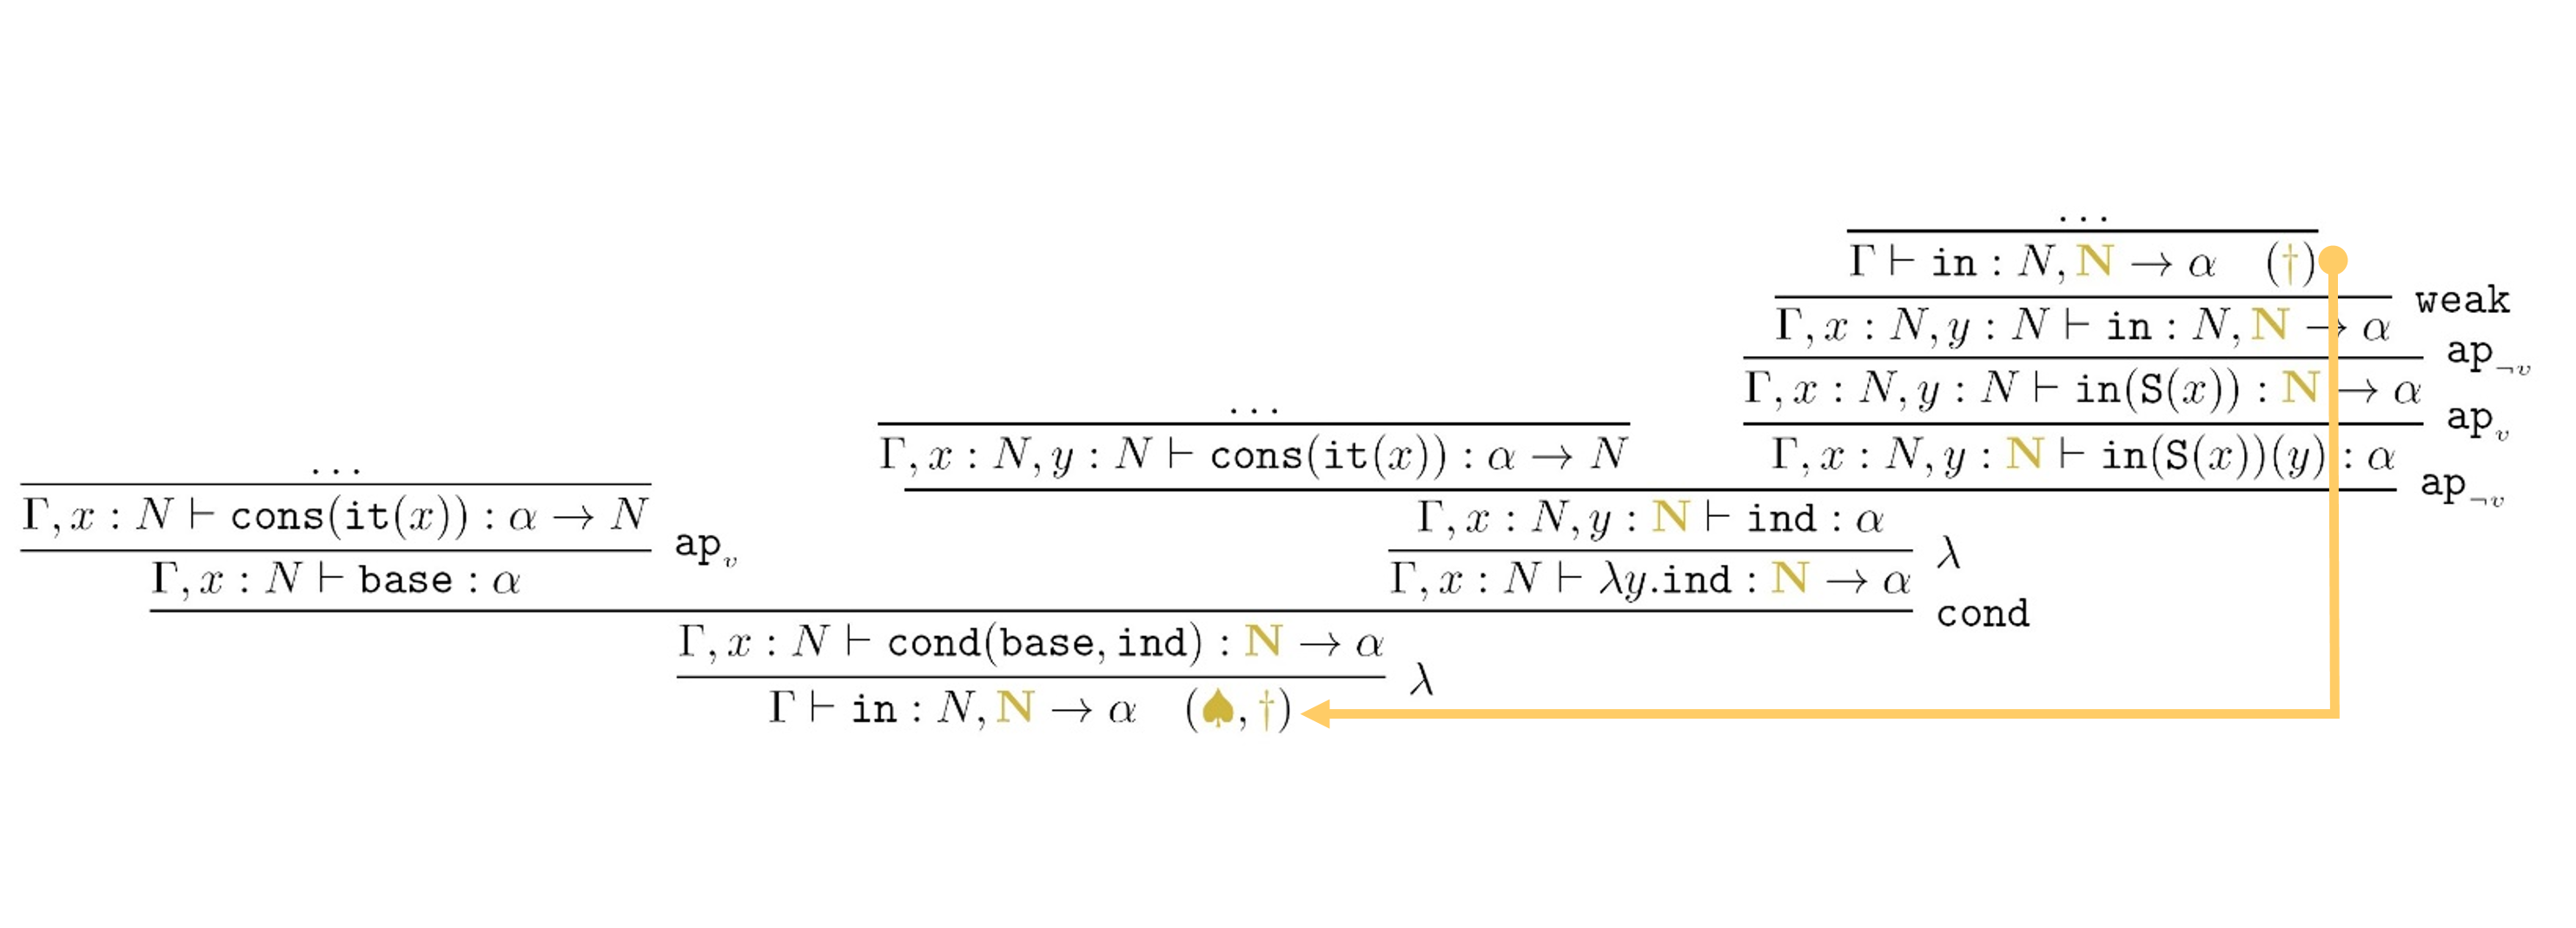
\includegraphics[scale=0.6]{type-inference-term-interval.PNG}

\begin{center}
%% LATEX SOURCE CODE THEN A SNAPSHOT 
%% THEN THE SNAPSHOT HAS BEEN MODIFIED IN WORD 
%% THEN A LAST SNAPSHOT
  
\[
%\infer[\lambda]
% {\Sigma\vdash \Interval:(\N \rightarrow \N),\N,\N,\bfColor{oldgold}{\N}\rightarrow\alpha}
% {\infer[\lambda]
%   {\Sigma,f:\N\rightarrow\N \vdash \lambda a.\interval:\N,\N,\bfColor{oldgold}{\N}   
%      \rightarrow\alpha}
   {\infer[\lambda]  
     {\Gamma \vdash \interval:\N,\bfColor{oldgold}{\N}\rightarrow\alpha 
       \ \ \ (\bfColor{oldgold}{\dagger}) }
       {\infer[\cond]{\Gamma, x:\N 
	\vdash 
	\cond (\base,  \inductive )
	:\bfColor{oldgold}{\N}\rightarrow\alpha \ \ \ (\bfColor{oldgold}{ \spadesuit}) } 
       {\infer[\apvar]{\Gamma, x:\N 
	           \vdash 
	           \base:\alpha}
             {\infer[]{\Gamma, x:\N 
	           \vdash 
	           \cons(\iter(x)):\alpha \rightarrow\N}{\ldots}}
            {\ \ \ \ \ \ }  &
          \infer[\lambda]{\Gamma, x:\N 
	           \vdash 
	           \lambda y.\inductive : \bfColor{oldgold}{\N}\rightarrow\alpha}
             {\infer[\apnotvar]{\Gamma, x:\N, y:\bfColor{oldgold}{\N} \vdash
               \inductive : \alpha}
            {\infer[]
                     {\Gamma, x:\N, y:\N 
                          \vdash \cons(\iter(x)):\alpha\rightarrow\N}{\ldots}
               {\ \ \ \ \ \ }
                     {\infer[\apvar]{\Gamma, x:\N, y:\bfColor{oldgold}{\N} 
                          \vdash \interval(\Succ(x))(y):\alpha}
                         {\infer[\apnotvar]{\Gamma, x:\N, y:\N 
                          \vdash \interval(\Succ(x)):\bfColor{oldgold}{\N} \rightarrow\alpha}
                              {\infer[\weak]{\Gamma, x:\N, y:\N 
                          \vdash \interval:\N,\bfColor{oldgold}{\N} \rightarrow\alpha}
                                {\infer[]{\Gamma 
                          \vdash \interval:\N,\bfColor{oldgold}{\N} \rightarrow\alpha
                           \ \ \ (\bfColor{oldgold}{\dagger})}
              {\ldots}}}}}
             }
           }
         }
       }  
    }
%   }
\]

\mbox{Figure \ref{figure-term-interval}}
\end{center}

\end{figure}

If we carefully examine the term $\Interval$, we can guess several results of this paper.
We have infinitely many nested $\beta$-reduction $(\lambda x. \ldots)(\Succ (x))$.
We can remove all of them in a single step. Inside the $\beta$-redex number $k$ we obtain a sub-term
$\iter[\Succ (x)/x]\ldots[\Succ (x)/x]$ (substitution repeated $k$ times).
The result is $\iter[\Succ ^k(x)/x] $.
The nested substitution produce infinitely many pairwise different sub-terms 
$\iter(\Succ ^k(x))$ for all $k \in \N$.
We need infinitely many steps to normalize all $\iter(\Succ ^k(x))$ to $f^k(I)$, 
even if we allow to reduce all $\beta,\cond$-redexes at the same time.
Also the normal form is not regular: it contains all terms $f^k(\iter(x))$ for $k \in \N$, hence
infinitely many pairwise different terms. 
%These infinite sub-terms are of a particulary simple form, though. 
%They are obtained by the repeating $k$ times the assignment $z:=f(z)$, then applying $z:=I$ once
%to the result.

In conclusion, 
$\Interval$ is some term of $\CTlambda$ which can be safely normalized, but which 
cannot be fully normalized in finite time, not even if we allow
infinite parallel reductions without any "safety" restriction. 
The normal form is produced \emph{only in the limit}
and it is \emph{not regular}. If we allow to reduce infinitely many nested existing
$\beta$-redexes in one step, also
the intermediate steps of the infinite reduction of $\Interval$ are not regular.


%16:32 30/04/2024
%22:30 03/06/2024




% Section 5
% !TEX root = main.tex

\section{Subject reduction for well-typed infinite lambda terms}
\label{section-subject-reduction}
 
We quickly quote the subject reduction property for well-typed terms of $\LAMBDA$,
and the fact that the global trace condition is preserved by subterms, substitution
and reductions. We skip proofs for reason of space, but they are just an exercise.
%We first introduce some auxiliary notations for proofs of them.
%
%Let $X$ be a set of variables of the form $x^T$.
%We write $\Gamma_X$ for the sublist of $\Gamma$ consisting of all $x^T:T$ such that $x^T\in X$. 
%Let $\Gamma$ and $\Delta$ be contexts of $\LAMBDA$.
%The merged context $\mergeCtx{\Gamma}{\Delta}$
%is defined by $\Gamma\conc(\Delta_{\FV(\Delta)\setminus\FV(\Gamma)})$. 
%
%Let $\theta$ be a renaming, and 
%$S_1 = \Gamma_1\vdash t_1:\vec{B_1}\rightarrow N$
%and $S_2 = \Gamma_2[\theta]\vdash t_2[\theta]:\vec{B_2}\rightarrow N$ be sequents. 
%Let $k_1$ and $k_2$ be indexes of $N$-arguments of $t_1$ and $t_2$, respectively. 
%Then we write $(k_1,S_1) \simIndex{\theta} (k_2,S_2)$ (or $(k_1,t_1) \simIndex{\theta} (k_2,t_2)$ for short)
%if they are respectively indexes of named arguments for some $y$ and $\theta(y)$, or
%are respectively those of unnamed arguments at the same position $i$ in $\vec{B_1}$ and $\vec{B_2}$,
%namely $k_1=|\Gamma_1|+i$ and $k_2=|\Gamma_2|+i$,
%where $|\Gamma_1|$ and $|\Gamma_2|$ are the sizes of $\Gamma_1$ and $\Gamma_2$. 
%Note that the index equivalent to $k_1$ is unique (if it exists), namely 
%$(k_1,t_1) \simIndex{\theta} (k_2,t_2)$ and $(k_1,t_1) \simIndex{\theta} (k'_2,t_2)$ implies $k_2=k'_2$.
%We write $(k_1,t_1) \simIndex{} (k_2,t_2)$ if $\theta$ is the identity renaming. 
%
%In this paper we do not implicitly identify $\alpha$-equivalent terms,
%in order to make simpler to state the global trace condition.
%For this reason, proofs of this section requires some delicate treatment of variables.
%
%We consider the following restricted $\lambda$ rule (called $\lambda'$) as follows:
%\begin{itemize}
%\item
%  $\lambda'$-rule.
%  If $\Gamma, x^A:A \vdash b: B$ and $\FV(\Gamma) = \FV(\lambda x.b)$, 
%  then $ \Gamma \vdash \lambda x^A.b :A \rightarrow B$.
%\end{itemize}
%
%The next lemma says that if $\Gamma\vdash t:A$ is provable,
%then $t:A$ can be shown in a restricted context $\Gamma_{\FV(t)}$
%even if the rule $\lambda$ is restricted to $\lambda'$. 
%
%\begin{lemma}\label{lem:thinning}
%  Assume $\Pi::\Gamma\vdash t:A$.
%  Then $\Pi'::\Gamma_{\FV(t)}\vdash t:A$ for some $\Pi'$ that may have instances of the rule $\lambda'$
%  and not have those of the rule $\lambda$.
%  Moreover if the global trace condition holds for $\Pi$, then it also holds for $\Pi'$. 
%\end{lemma}
%
%%\begin{proof}
%%  First we call the following admissible rule $\lambda'\weak$:
%%  \begin{itemize}
%%  \item
%%    $\lambda'\weak$-rule.
%%    If $\Gamma, x^A:A \vdash b: B$, $\FV(\Gamma) = \FV(\lambda x.b)$ and $\Gamma\subseteqsim \Gamma'$, 
%%    then $ \Gamma' \vdash \lambda x^A.b :A \rightarrow B$.
%%  \end{itemize}
%%  We write $\Rule'$ as the set of rule instances obtained by removing
%%  those of $\lambda$ from $\Rule$ and adding those of $\lambda'\weak$. 
%%  Note that if we have a proof of a sequent with $\lambda'\weak$,
%%  then we also have a proof of the same sequent not with $\lambda'\weak$
%%  by a proof transformation that splits each $\lambda'\weak$ by $\lambda'$ and $\weak$. 
%%  Also note that this proof transformation preserves the global trace condition.
%%
%%  Let $\Pi$ be $(T,\phi)$.
%%  For each $l \in T$, we write $\Gamma_l\vdash t_l:A_l$
%%  for the conclusion of $\phi(l) \in \Rule$. 
%%  To show the lemma, from a given proof $\Pi$, 
%%  it is enough to construct a proof $\Pi'$ of $\Restrict{\Gamma}{\FV(t)}\vdash t:A$ with $\Rule'$.
%%  
%%  We define the set of nodes of $\Pi'$ is $T$, which is the same one of $\Pi$. 
%%  For each $l\in T$, we define $\phi'(l)$ and $\Gamma'_l$ that satisfies
%%  the following requirements:
%%  \begin{itemize}
%%  \item[(a)]
%%    $\Gamma'_l\vdash t_l:A_l$ is the conclusion of $\phi'(l) \in \Rule'$,
%%  \item[(b)]
%%    $\Restrict{(\Gamma_l)}{\FV(t_l)} \subseteqsim \Gamma'_l \subseteqsim \Gamma_l$
%%    and $\Gamma'_{\nil} = \Restrict{\Gamma}{\FV(t)}$, 
%%  \item[(c)]
%%    if $\tilde{k},t_{l\conc(i)}$ is the successor of $k,t_l$ in $\Pi$
%%    and $k$ is an index of some unname argument
%%    or a named argument of some name $z\in\FV(t_l)$, 
%%    then there are $\tilde{k'}$ and $k'$ such that
%%    $\tilde{k'},t_{l\conc(i)}$ is the successor of $k',t_l$ in $\Pi'$, 
%%    $(k,t_l) \simIndex{} (k',t_l)$,
%%    and $(\tilde{k},t_{l\conc(i)}) \simIndex{} (\tilde{k'},t_{l\conc(i)})$.
%%    Moreover, if $k$ is an index of a progressing argument, then so is $k'$.
%%  \end{itemize}
%%  Note that the proof is done if we construct $\Pi'$ that satisfies these requirements. 
%%  
%%  We define $\Gamma'_{\nil} = \Restrict{\Gamma}{\FV(t)}$.
%%  Then it satisfies (b) since $t_\nil = t$. 
%%  Next, assuming the induction hypothesis that $\Gamma'_l$ which satisfies (b)
%%  is already defined, 
%%  we define $\phi'(l)$ and $\Gamma_{l\conc(i)}$, 
%%  for each $i$ such that $l\conc(i)\in T$, 
%%  that satisfies (a), (b), and (c). 
%%  It is done by the case analysis of $\phi(l)$.
%%
%%  The case of $\phi(l) = \Gamma_l\vdash x:A_l$,
%%  which is an instance of the rule $\var$ with $x:A_l\in\Gamma_l$. 
%%  Then define $\phi'(l) = \Gamma'_l\vdash x:A_l$. This is an instance of $\var$
%%  because $x:A_l \in \Restrict{(\Gamma_l)}{\FV(x)} \subseteqsim \Gamma'_l$ by (b).
%%
%%  The case of $\phi(l) = (\Gamma_{l\conc(1)}\vdash t_l:A_l,\Gamma_{l}\vdash t_l:A_l)$,
%%  which is an instance of the rule $\weak$ with
%%  $t_{l\conc(1)} = t_l$, $A_{l\conc(1)} = A_{l}$, and
%%  $\Gamma_{l\conc(1)}\subseteqsim \Gamma_l$.
%%  Let $\psi$ be the unique map that determines $\Gamma_{l\conc(1)}\subseteqsim \Gamma_l$.
%%  Then define $\Gamma'_{l\conc(1)}$ such that
%%  $\Gamma'_{l\conc(1)}\subseteqsim \Gamma'_l$ determined by
%%  the induced map from $\psi$ restricting the range to $\FV(\Gamma'_l)$.
%%  Note that $\FV(\Gamma'_{l\conc(1)}) = \FV(\Gamma'_l)\cap\FV(\Gamma_{l\conc(1)})$. 
%%  Then it satisfies (b) since $\FV(t_l)\subseteq \FV(\Gamma'_l) \cap \FV(\Gamma_{l\conc(1)}) = \FV(\Gamma'_{l\conc(1)}) \subseteq \FV(\Gamma_{l\conc(1)})$ by (b) for $\Gamma'_l$.
%%  Define $\phi'(l) = (\Gamma'_{l\conc(1)}\vdash t_l:A_l,\Gamma'_{l}\vdash t_l:A_l)$
%%  as an instance of the rule $\weak$. 
%%  Hence the requirement (a) holds.
%%  We can also show (c): if $k$ is an index in $\Gamma_l\vdash t_l:A_l$ for a name
%%  $z\in\FV(t_{l\conc(1)}) = \FV(t_l)$, then we can take an index $k'$
%%  in $\Gamma'_l\vdash t_l:A_l$ for $z$ by $\FV(t_l)\subseteq\FV(\Gamma'_l)$ by (b). 
%%  An index $\tilde{k'}$ for the name $z$ can be taken
%%  from $\Gamma'_{l\conc(1)}\vdash t_l:A_l$
%%  since $z \in \FV(t_l) \subseteq \FV(\Gamma'_{l\conc(1)})$. 
%%  
%%  The case of $\phi(l) = (\Gamma_l,z:C\vdash b:\vec{B}\to N, \Gamma_l\vdash\lambda z^C.b:C,\vec{B}\to N)$
%%  that is an instance of the rule $\lambda$. 
%%  Define $\Gamma'_{l\conc(1)} = \Restrict{(\Gamma_l)}{\FV(\lambda z.b)},z:C$ and 
%%  $\phi'(l) = (\Restrict{(\Gamma_l)}{\FV(\lambda z.b)},z:C\vdash b:\vec{B}\to N, \Gamma'_l\vdash \lambda z.b:C,\vec{B}\to N)$. 
%%  This is an instance of the rule $\lambda'\weak$, since $\Restrict{(\Gamma_l)}{\FV(\lambda z.b)}\subseteqsim \Gamma'_l$ by the induction hypothesis.
%%  Trivially we have (a). 
%%  We also have (b) by $\Restrict{(\Gamma_l,z:C)}{\FV(b)} \subseteqsim (\Restrict{(\Gamma_l)}{\FV(\lambda z.b)},z:C) \subseteqsim (\Gamma_l,z:C)$.   
%%  The requirement (c) holds: 
%%  if $k$ is an index of some named argument $y\in\FV(\lambda z.b)$ in $\Gamma_l$,
%%  then $k'$ can be taken as the index of $y$ in $\Gamma'_l$ by (b) for $\Gamma_l$.
%%  If $k$ is an index of some unnamed argument in $C,\vec{B}$,
%%  then $k'$ can be taken as the index of some unnamed argument. 
%%  In both cases, their successors $\tilde{k}$ and $\tilde{k'}$ are uniquely
%%  determined by $k$ and $k'$, respectively. 
%%  
%%  The case that $\phi(l)$ is an instance of the rule $\apvar$
%%  whose conclusion is $\Gamma_l\vdash f(x^B):\vec{C}\to N$ with $x:B\in \Gamma_l$.  
%%  Define $\Gamma'_{l\conc(1)} = \Gamma'_l$.
%%  This satisfies (b) by the induction hypothesis. 
%%  Then define
%%  $\phi'(l) = (\Gamma'_{l\conc(1)}\vdash f:B,\vec{C}\to N, \Gamma'_l\vdash f(x^B):\vec{C}\to N)$
%%  as an instance of the rule $\apvar$. This satisfies (a). 
%%  In order to show (c), 
%%  take an index $k$ for $\Gamma_l\vdash f(x^B):\vec{C}\to N$, which is the one for
%%  a named argument $y \in \FV(f(x^B))$ in $\Gamma_l$
%%  or for some unnamed argument of $\vec{C}$. 
%%  For the latter case, the indexes $\tilde{k}$, $k'$ and $\tilde{k'}$ can be taken
%%  as those of the unnamed argument in $\vec{C}$ at the same position as $k$.
%%  For the former case, we take $k'$ as the index for $y$ in $\Gamma'_l$.
%%  In order to take $\tilde{k'}$,
%%  we further have two subcases according to $\tilde{k}$: 
%%  The first one is $\tilde{k}$ is the index for the same named argument as $k$, 
%%  and the second one is $\tilde{k}$ is the index for the unnamed argument, namely $B=N$.
%%  In both subcases, we can take the equivalent $\tilde{k'}$ to $\tilde{k}$ as we wished.
%%    
%%  The case that $\phi(l)$ is an instance of the rule $\apnotvar$
%%  whose conclusion is $\Gamma_l\vdash f(b^B):A_l$. 
%%  Define $\Gamma'_{l\conc(1)} = \Gamma'_{l\conc(2)} = \Gamma'_l$.
%%  This satisfies (b) by the induction hypothesis.
%%  Then define $\phi'(l) = (S_1, S_2, \Gamma'_l\vdash f(b^B):\vec{C}\to N)$,
%%  where $S_1$ is $\Gamma'_{l}\vdash f:B,\vec{C}\to N$
%%  and $S_2$ is $\Gamma'_{l}\vdash b:B$, as an instance of $\apnotvar$.
%%  This satisfies (a).
%%  In order to show (c), 
%%  take an index $k$ for $\Gamma_l\vdash f(x^B):\vec{C}\to N$, which is the one for
%%  a named argument $y \in \FV(f(x^B))$ in $\Gamma_l$
%%  or for some unnamed argument of $\vec{C}$.
%%  For the former case, the successor $\tilde{k}$ of $k$ is uniquely taken.
%%  By $\FV(f(b)) \subseteq \FV(\Gamma'_l)$, the index $k'$ equivalent to $k$ is uniquely taken. 
%%  Then the successor $\tilde{k'}$ of $k'$ is also taken as we wished. 
%%  For the latter case, the successor $\tilde{k}$ of $k$ is uniquely taken
%%  as the one for unnamed argument at the same position as $k$. 
%%  Then $k'$ equivalent to $k$ is uniquely taken, and 
%%  its successor $\tilde{k'}$ is also taken as we wished. 
%%
%%  The case that $\phi(l)$ is an instance of the rule $0$
%%  whose conclusion is $\Gamma_l\vdash 0:N$. 
%%  Define $\phi'(l) = \Gamma'_l\vdash 0:N$ as an instance of the rule $0$.
%%  This satisfies the requirements (a), (b), and (c). 
%%
%%  The case that $\phi(l)$ is an instance of the rule $\Succ$
%%  whose conclusion is $\Gamma_l\vdash \Succ(t_{l\conc(1)}):N$ with $A_l=N$.
%%  Define $\Gamma'_{l\conc(1)} = \Gamma'_l$, and 
%%  $\phi'(l) = (\Gamma'_l\vdash t_{l\conc(1)}:N, \Gamma'_l\vdash \Succ(t_{l\conc(1)}):N)$
%%  as an instance of $\Succ$. They satisfy (a) and (b). 
%%  The requirement (c) is also satisfied:
%%  Take an index $k$ for $\Gamma_l\vdash \Succ(t_{l\conc(1)}): N$,
%%  which is the one for a named argument $y \in \FV(\Succ(t_{l\conc(1)})$ in $\Gamma_l$.
%%  Then the successor $\tilde{k}$ of $k$ is uniquely taken.  
%%  By $\FV(t_{l\conc(1)}) \subseteq \FV(\Gamma'_l)$, the index $k'$ equivalent to $k$ is uniquely taken. 
%%  Then the successor $\tilde{k'}$ of $k'$ is also taken as we wished. 
%%  
%%  The case that $\phi(l)$ is an instance of the rule $\cond$
%%  whose conclusion is $\Gamma_l\vdash \cond(f,g):N,\vec{C}\to N$. 
%%  Define $\Gamma'_{l\conc(1)} = \Gamma'_{l\conc(2)} = \Gamma'_l$, and 
%%  $\phi'(l) = (S_1,S_2, \Gamma'_l\vdash \cond(f,g):N,\vec{C}\to N)$,
%%  where $S_1$ is $\Gamma'_l\vdash f:\vec{C}\to N$ and $S_2$ is $\Gamma'_l \vdash g:N,\vec{C}\to N$, 
%%  as an instance of $\cond$. They satisfy (a) and (b). 
%%  To show (c), take an index $k$ for $\Gamma_l\vdash \cond(f,g): N,\vec{C}\to N$ as required. 
%%  We need to consider three cases:
%%  $k$ is the index for a named argument $y \in \FV(\cond(f,g))$ in $\Gamma_l$,
%%  is the one for an unnamed argument in $\vec{C}$, or
%%  is the one for an unnamed argument in $N$ (the first one of $N,\vec{C}\to N$). 
%%  For the first and second cases, we can take $\tilde{k}$, $k'$, and $\tilde{k'}$
%%  similar to the other cases.
%%  For the last case, the successor $\tilde{k}$ of $k$ should be taken
%%  as the index of the unnamed $N$-argument of $\Gamma'_l \vdash g:N,\vec{C}\to N$
%%  at the same position as $k$. 
%%  Then $k'$ and $\tilde{k'}$ are taken as those equivalent to $k$ and $\tilde{k}$, respectively.
%%  Note that this $k$ is an index of a progressing argument $N$, and so is $k'$. 
%%\end{proof}
%%
%%
%
%\begin{lemma}[Substitution lemma]
%  Assume that $\Pi_u:: \Delta \vdash u:A$ and $\Pi_t::\Gamma,x:A \vdash t:B$ hold. 
%  Then there exists $\Pi^\circ$ such that $\Pi^\circ::\mergeCtx{\Delta}{\Gamma} \vdash t[u/x]:B$. 
%  Moreover, if both $\Pi_u$ and $\Pi_t$ satisfy the global trace condition,
%  then $\Pi^\circ$ also satisfies it. 
%\end{lemma}
%
%
%%\begin{proof}
%%  Assume that $\Pi_u:: \Delta \vdash u:A$ and $\Pi_t::\Gamma,x:A \vdash t:B$ hold. 
%%  By Lemma~\ref{lem:thinning}, without loss of generality,
%%  we can assume $\FV(\Delta) = \FV(u)$ and $\Pi_t$ is a proof with the restricted $\lambda$ rule (the $\lambda'$ rule). 
%%  Let $\Pi_u=(T_u,\phi_u)$ and $\Pi_t=(T_t,\phi_t)$.
%%  For each $l\in T_t$, we write $\Gamma_l\vdash t_l:C_l$
%%  for the conclusion of $\phi_t(l)$.
%%  We use $\xx$ to mark occurences of $x$ in $\Pi_t$ that connects
%%  with the explicit $\xx$ of $\Gamma,\xx:A\vdash t:B$. 
%%  In the following, we construct a proof $\Pi^\circ = (T^\circ,\phi^\circ)$ of
%%  $\mergeCtx{\Delta}{\Gamma}\vdash t[u/x]:B$ such that 
%%  \begin{itemize}
%%  \item[(a1)]
%%    $T^\circ = T_t \cup T_{\var} \cup T_{\apvar}$, where
%%    $T_{\var} = \{l\conc(1)\conc l' \mid \text{$l\in T_t$, $\phi(l)=\var$ of $\xx$, and $l'\in T_u$} \}$
%%    and
%%    $T_{\apvar} = \{l\conc(2)\conc l' \mid \text{$u$ is not a variable, $l\in T_t$, $\phi(l)=\apvar$ of $f(\xx)$ for some $f$, and $l'\in T_u$}\}$.
%%    The explicit $1$ of $l\conc(1)\conc l' \in T_\var$ is called the switching point of $l\conc(1)\conc l'$.
%%    The explicit $2$ of $l\conc(2)\conc l' \in T_\apvar$ is also called the switching point of $l\conc(2)\conc l'$.     \item[(a2)]
%%    For each $l\conc(i)\conc l' \in T_\var \cup T_\apvar$ with switching point $i$,
%%    we have $\phi^\circ(l\conc(i)\conc l') = \phi_u(l')$. 
%%  \end{itemize}
%%  Moreover, for all $l \in T_t$,
%%  the rule instance $\phi^\circ(l)$ satisfies the following requirements
%%  with an auxiliary function $\sigma^\circ:T_t \to \Seq$ and a substitution $\theta_l$: 
%%  \begin{itemize}
%%  \item[(b1)]
%%    The sequent $\sigma^\circ(l)$ has the form $\Gamma^\circ_l\vdash t_l[\theta_l]:C_l$.
%%    The substitution $\theta_l$ is $\{u/\xx\}\cup\theta_{{\rm ren}}$
%%    if $\xx:A \in \Gamma_l$, and is $\theta_{{\rm ren}}$ otherwise, 
%%    where $\theta_{{\rm ren}}$ is some renaming.
%%    $\Gamma^\circ_l \sim \Delta_l\sharp\Restrict{(\Gamma_l)}{\overline{\xx}}[\theta_l]$ holds,
%%    where $\Delta_l$ is $\Delta$ if $\xx:A\in\Gamma_l$, and is $\emptyset$ otherwise. 
%%  \item[(b2)]
%%    $\sigma^\circ(l)$ is the conclusion of $\phi^\circ(l)$,
%%    and $\sigma^\circ(l\conc(i))$ is the $i$-th assumption of $\phi^\circ(l)$ if $l\conc(i) \in T_t$.
%%  \item[(b3)]
%%    Assume $\tilde{k},t_{l\conc(i)}$ is a successor of $k,t_l$ and $k$ is not a named index for $\xx$. 
%%    Then there exist $\tilde{k^\circ}$ and $k^\circ$ such that
%%    $\tilde{k^\circ},t_{l\conc(i)}[\theta_{l\conc(i)}]$ is a successor of $k^\circ,t_l[\theta_l]$ and 
%%    $(k,t_l) \simIndex{\Restrict{(\theta_l)}{\overline{\xx}}} (k^\circ,t_l[\theta_l])$.
%%    If $k$ is an index of a progressing argument, then so is $k^\circ$.    
%%  \end{itemize}
%%  
%%  Note that if we have $\Pi^\circ$ that satisfies the requirements, its possibly infinite path
%%  is a path of $\Pi_t$ or a path of $\Pi_u$ or a path $l\conc(i)\conc l'$,
%%  where $l$ is a path of $T_t$, $i$ is a switching point, and $l'$ is a path of $T_u$.
%%  Hence $\Pi^\circ$ is Almost-left-finite, since $\Pi_t$ and $\Pi_u$ are Almost-left-finite.
%%  In addition, if $\Pi_t$ and $\Pi_u$ satisfies the global trace condition,
%%  so does $\Pi^\circ$ by (b3). 
%%  Therefore, to complete the proof, it is enough to construct $\Pi^\circ$. 
%%
%%  First, for each $l\conc(j)\conc l'\in T_\var\cup T_\apvar$ with a switching point $j$, 
%%  we define $\phi^\circ(l\conc(j)\conc l') = \phi_u(l')$. 
%%
%%  In the following, for each $l\in T_t$, we inductively define $\Gamma^\circ_l$, $\phi^\circ(l)$, and $\sigma(l)$
%%  that satisty (b1), (b2), and (b3).
%%  The case of $l=\nil$, define $\Gamma^\circ_\nil = \Delta\sharp\Gamma$ and $\theta_\nil=\{u/\xx\}$,
%%  and define $\sigma^\circ(\nil)$ as $\mergeCtx{\Delta}{\Gamma}\vdash t[u/\xx]:A$. 
%%  Hence we have (b1) since
%%  $\Gamma^\circ_\nil = \mergeCtx{\Delta}{\Gamma} \sim \mergeCtx{\Delta}{\Restrict{(\Gamma,\xx:A)}{\overline{\xx}}[\theta_\nil]}$. 
%%
%%  For each $l\in T_t$,
%%  with the induction hypothesis that $\sigma^\circ(l)$ and $\theta_l$ that satisfy (b1) are already defined, 
%%  we define $\phi^\circ(l)$, and define $\theta_{l\conc(i)}$ and $\sigma^\circ(l\conc(i))$ when $l\conc(i)\in T_t$, 
%%  such that they satisfy (b1), (b2), and (b3). 
%%  We perform this by the case analysis of $\phi(l)$.
%%
%%  The case $\phi(l)= (\Gamma_l\vdash \xx:A)$ that is an instance of $\var$.
%%  We can define $\phi^\circ(l) = (\Delta\vdash u:A, \Gamma^\circ_l\vdash u:A)$ as $\weak$,
%%  since $\Delta\subseteqsim \mergeCtx{\Delta}{\Restrict{(\Gamma_l)}{\overline{\xx}}[\theta_l]} \sim \Gamma^\circ_l$
%%  holds by (b1). 
%%  As $l\conc(i)\not\in T_t$, (b1), (b2), and (b3) trivially hold.
%%  
%%  The case $\phi(l) = (\Gamma_l\vdash y:B)$ that is an instance of $\var$ with $y \neq \xx$. 
%%  We can define $\phi^\circ(l) = (\Gamma^\circ_l\vdash \theta_l(y):B)$ as $\var$,
%%  since $\theta_l(y):B \in \Restrict{(\Gamma_l)}{\overline{\xx}}[\theta_l] \subseteqsim \mergeCtx{\Delta_l}{\Restrict{(\Gamma_l)}{\overline{\xx}}[\theta_l]} \sim \Gamma^\circ_l$ holds by (b1).
%%  As $l\conc(i)\not\in T_t$, (b1), (b2), and (b3) trivially hold.
%%
%%  The case $\phi(l) = (S_1,S_2,\Gamma_l\vdash f(b):C)$ that is an instance of $\apnotvar$,
%%  where $S_1 = \Gamma_l\vdash f:B\to C$, $S_2 = \Gamma_l\vdash b:B$, and $b$ is not a variable. 
%%  Define $\phi^\circ(l) = (S'_1, S'_2,\Gamma^\circ_l\vdash f[\theta_l](b[\theta_l]):C)$ as $\apnotvar$, 
%%  where $S'_1 = \Gamma^\circ_l\vdash f[\theta_l]:B\to C$ and $S'_2 = \Gamma^\circ_l\vdash b[\theta_l]:B$,
%%  since $b[\theta_l]$ is not a variable.
%%  Also define $\sigma^\circ(l\conc(1)) = S'_1$, $\sigma^\circ(l\conc(2)) = S'_2$,
%%  and $\theta_{l\conc(1)} = \theta_{l\conc(2)} = \theta_l$. 
%%  Then (b1) and (b2) trivially hold.
%%  To check (b3),
%%  assume that $\tilde{k},t$ is a successor of $k,f(b)$, where $t$ is $f$ or $b$,
%%  and $k$ is not a named index for $\xx$.
%%  Then (i) both $k$ and $\tilde{k}$ are named indexes for some variable $y^D\in\Dom(\Gamma_l)$,
%%  (ii) both $k$ and $\tilde{k}$ are unnamed indexes in $C$. 
%%  For the case (ii), take $k'$ and $\tilde{k'}$ as the same indexes as $k$ and $\tilde{k}$, respectively.
%%  For the case (i), we have
%%  $\theta_l(y):D \in \Restrict{(\Gamma_l)}{\overline{\xx}}[\theta_l] \subseteqsim \Gamma^\circ_l \subseteqsim \Gamma^\circ_{l\conc(1)}$ 
%%  by $y \neq \xx$. Then take $k'$ and $\tilde{k'}$ as named indexes for $\theta_l(y)$.
%%  In each case, $k'$ and $\tilde{k'}$ satisfy (b3) as expected. 
%%  
%%  The case $\phi(l) = (S_1,\Gamma_l\vdash f(\xx):C)$ that is an instance of $\apvar$, 
%%  where $S_1 = \Gamma_l \vdash f:A\to C$ and $\xx:A\in\Gamma_l$. 
%%  We need to consider the two subcases whether $u$ is a variable or not.
%%  \begin{itemize}
%%  \item
%%    If $u$ is a variable $y^B$, 
%%    we can define $\phi^\circ(l) = (S'_1, \Gamma^\circ_l\vdash f[\theta_l](y):C)$,
%%    where $S'_1 = \Gamma^\circ_l\vdash f[\theta_l]:A\to C$ as $\apvar$,
%%    since
%%    $y:B \in \Delta \subseteqsim \mergeCtx{\Delta}{\Restrict{(\Gamma_l)}{\overline{\xx}}[\theta_l]} \sim \Gamma^\circ_l$
%%    holds by (b1). 
%%    Also define $\sigma^\circ(l\conc(1)) = S'_1$ and $\theta_{l\conc(1)} = \theta_l$. 
%%    Then (b1) and (b2) trivially hold. (b3) is checked in a similar way to the case $\apnotvar$.
%%  \item
%%    If $u$ is not a variable, 
%%    define $\phi^\circ(l) = (S'_1, S'_2, \Gamma^\circ_l\vdash f[\theta_l](u):C)$,
%%    where
%%    $S'_1 = \Gamma^\circ_l\vdash f[\theta_l]:A\to C$ and
%%    $S'_2 = \Gamma^\circ_l\vdash u:A$ as $\apnotvar$. 
%%    Also define $\sigma^\circ(l\conc(1)) = S'_1$, $\sigma^\circ(l\conc(2)) = S'_2$,
%%    and $\theta_{l\conc(1)} = \theta_{l\conc(2)} = \theta_l$. 
%%    Then (b1) and (b2) trivially hold. (b3) is checked in a similar way to the case of $\apnotvar$. 
%%  \end{itemize}
%%
%%  The case $\phi(l) = (S_1,\Gamma_l\vdash f(y):C)$
%%  that is an instance of $\apvar$, where $S_1 = \Gamma_l \vdash f:B \to C$, $y:B\in\Gamma_l$ and $y\neq \xx$. 
%%  We can define $\phi^\circ(l) = (S'_1, \Gamma^\circ_l\vdash f[\theta_l](\theta_l(y)):C)$ as $\apvar$,
%%  where $S'_1 = \Gamma^\circ_l\vdash f[\theta_l]:B\to C$, 
%%  since
%%  $\theta_l(y):B \in \Restrict{(\Gamma_l)}{\overline{\xx}}[\theta_l] \subseteqsim \mergeCtx{\Delta_l}{\Restrict{(\Gamma_l)}{\overline{\xx}}[\theta_l]} \sim \Gamma^\circ_l$
%%  holds by (b1). 
%%  Also define $\sigma^\circ(l\conc(1)) = S'_1$ and $\theta_{l\conc(1)} = \theta_l$. 
%%  Then (b1) and (b2) trivially hold. (b3) is checked in a similar way to the case $\apnotvar$.
%%  
%%  The case $\phi(l) = (\Gamma_l, z:C\vdash b:B,\Gamma_l\vdash \lambda z.b:C\to B)$
%%  that is an instance of $\lambda'$. 
%%  By the assumption, we have $\theta_l$
%%  and $\sigma^\circ(l)=\Gamma^\circ\vdash (\lambda z.b)[\theta_l]:C\to B$ that satisfy (b1).
%%  Let $\theta_l=\{\vec{u}/\vec{x}\}$. 
%%  We consider two subcases.
%%  \begin{itemize}
%%  \item
%%    The first subcase is when $z\not\in\FV(\vec{u})$.
%%    We have $(\lambda z.b)[\theta_l] = \lambda z.(b[\Restrict{(\theta_l)}{\overline{z}}])$.
%%    Then define $\phi^\circ(l) = (\Gamma^\circ_l, z:C\vdash b[\Restrict{(\theta_l)}{\overline{z}}]:B,\Gamma^\circ_l\vdash \lambda z.(b[\Restrict{(\theta_l)}{\overline{z}}]):C\to B)$ as $\lambda$. 
%%    Note that $\Gamma^\circ_l,z:C$ is a context 
%%    because $z:C \not\in \mergeCtx{\Delta_l}{\Restrict{(\Gamma_l)}{\overline{\xx}}[\theta_l]} \sim \Gamma^\circ_l$
%%    holds by (b1), $z\not\in \FV(\Gamma_l)$ and $z \not\in\FV(\vec{u}) \supseteq \FV(\Delta_l)$
%%    (recall that $\Delta_l$ is $\Delta$ when $\xx:A\in\Gamma_l$, and is $\emptyset$ otherwise).
%%    Define $\sigma^\circ(l\conc(1)) = \Gamma^\circ_l,z:C\vdash b[\Restrict{(\theta_l)}{\overline{z}}]:B$
%%    and $\theta_{l\conc(1)} = \Restrict{(\theta_l)}{\overline{z}}$.
%%    We have (b2) by the definition. 
%%    We also have (b1) by $(\Gamma^\circ_l,z:C) \sim (\mergeCtx{\Delta_l}{\Restrict{(\Gamma_l)}{\overline{\xx}}}[\theta_l],z:C) = \mergeCtx{\Delta_l}{\Restrict{(\Gamma_l,z:C)}{\overline{\xx}}}[\theta_{l\conc(1)}]$.
%%    To check (b3),
%%    assume that $\tilde{k},b$ is a successor of $k,\lambda z.b$ and $k$ is not a named index for $\xx$.
%%    Then (i) both $k$ and $\tilde{k}$ are named indexes for some variable $y^D\in\Dom(\Gamma_l)$,
%%    (ii) both $k$ and $\tilde{k}$ are unnamed indexes (not for $C$), or
%%    (iii) $k$ is an unnamed indexes for $C$ and $\tilde{k}$ is a named index for $z$.
%%    The cases (i) and (ii) can be checked in a similar way to the case of $\apnotvar$.
%%    The case (iii) is checked by taking $k'$ and $\tilde{k'}$ as the same indexes as $k$ and $\tilde{k}$,
%%    respectively.
%%  \item
%%    The second subcase is when $z\in\FV(\vec{u})$.
%%    We have $(\lambda z.b)[\theta_l] = \lambda z'.(b[\Restrict{(\theta_l)}{\overline{z}},z'/z])$, 
%%    where $z' \not\in\FV(b,\vec{u})$. 
%%    Then define $\phi^\circ(l) = (\Gamma^\circ_l, z':C\vdash b[\Restrict{(\theta_l)}{\overline{z}},z'/z]:B,\Gamma^\circ_l\vdash \lambda z'.(b[\Restrict{(\theta_l)}{\overline{z}},z'/z]):C\to B)$ as $\lambda$. 
%%    We need to check that $\Gamma^\circ_l,z':C$ is a context.
%%    It is shown by
%%    $z':C \not\in \mergeCtx{\Delta_l}{\Restrict{(\Gamma_l)}{\overline{\xx}}[\theta_l]} \sim \Gamma^\circ_l$
%%    using (b1), 
%%    $z'\not\in \FV(\lambda z.b) = \FV(\Gamma_l)$ and $z' \not\in\FV(\vec{u}) \supseteq \FV(\Delta_l)$. 
%%    Define $\sigma^\circ(l\conc(1)) = \Gamma^\circ_l,z':C\vdash b[\Restrict{(\theta_l)}{\overline{z}},z'/z]:B$
%%    and $\theta_{l\conc(1)} = \Restrict{(\theta_l)}{\overline{z}}\cup\{z'/z\}$.
%%    We have (b2) by the definition. 
%%    We also have (b1) by $(\Gamma^\circ_l,z':C) \sim (\mergeCtx{\Delta_l}{\Restrict{(\Gamma_l)}{\overline{\xx}}}[\theta_l],z':C) = \mergeCtx{\Delta_l}{\Restrict{(\Gamma_l,z:C)}{\overline{\xx}}}[\theta_{l\conc(1)}]$.
%%    Checking (b3) is done in a similar way to that of the first subcase.
%%  \end{itemize}
%%
%%  The case $\phi(l) = (S_1,S_2,\Gamma_l\vdash \cond(f,g):\N\to C)$, where
%%  $S_1 = \Gamma_l\vdash f:C$, $S_2 = \Gamma_l\vdash g:\N\to C$, as an instance of $\cond$. 
%%  Define $\phi^\circ(l) = (S'_1,S'_2,\Gamma^\circ_l\vdash \cond(f[\theta_l],g[\theta_l]):\N\to C)$ as $\cond$,
%%  where $S'_1 = \Gamma^\circ_l \vdash f[\theta_l]:C$ and $S'_2 = \Gamma^\circ_l \vdash g[\theta_l]:\N\to C$.
%%  Also define $\sigma^\circ(l\conc(1)) = S'_1$, $\sigma^\circ(l\conc(2))  = S'_2$,
%%  and $\theta_{l\conc(1)} = \theta_{l\conc(2)} = \theta_l$. 
%%  Then (b1) and (b2) trivially hold.
%%  (b3) is checked in a similar way to the case of $\apnotvar$.
%%
%%  The case $\phi(l) = (\Gamma_l\vdash 0:\N)$, as an instance of $0$. 
%%  Define $\phi^\circ(l) = (\Gamma^\circ_l\vdash 0:\N)$ as $0$. 
%%  Since $l\conc(i)\not\in T_t$, (b1), (b2), and (b3) trivially hold.
%%  
%%  The case $\phi(l) = (\Gamma_l\vdash t:\N, \Gamma_l\vdash \Succ(t):\N)$, as an instance of $\Succ$. 
%%  Define
%%  $\phi^\circ(l) = (\Gamma^\circ_l\vdash t[\theta_l]:\N, \Gamma^\circ_l\vdash \Succ(t[\theta_l]):\N)$ as $\Succ$. 
%%  Also define $\sigma^\circ(l\conc(1)) = \Gamma^\circ_l\vdash t:\N$
%%  and $\theta_{l\conc(1)} = \theta_l$.
%%  Then (b1) and (b2) trivially hold.
%%  (b3) is checked in a similar way to the case of $\apnotvar$.
%%
%%  Therefore our construction of $\Pi^\circ$ is completed.
%%\end{proof}
%%
%%
%

\begin{lemma}[Inversion Lemma]\label{lem:inversion}
  \begin{enumerate}
  \item\label{lem:inversion1}
    If $\Pi::\Gamma\vdash f(a):A$ and $\Pi$ satisfies the global trace condition, then
    there exist $\Pi_1$, $\Pi_2$ and $B$ such that
    $\Pi_1::\Gamma\vdash f:B\to A$, $\Pi_2::\Gamma\vdash a:B$,
    and both $\Pi_1$ and $\Pi_2$ satisfy the global trace condition. 
  \item\label{lem:inversion2}
    If $\Pi::\Gamma\vdash \lambda x^T.b:A$, where $x\not\in\FV(\Gamma)$,
    and $\Pi$ satisfies the global trace condition, then
    there exist $\Pi_1$ and $B$ such that
    $\Pi_1::\Gamma,x:T\vdash b:B$ and $A = T\to B$,
    and $\Pi_1$ satisfies the global trace condition. 
  \item\label{lem:inversion3}
    If $\Pi::\Gamma\vdash \cond(f,g):A$ and $\Pi$ satisfies the global trace condition, then
    there exist $\Pi_1$, $\Pi_2$ and $B$ such that
    $\Pi_1::\Gamma \vdash f:B$, $\Pi_2:\Gamma \vdash g:N\to B$, $A = N\to B$,
    and both $\Pi_1$ and $\Pi_2$ satisfy the global trace condition. 
  \item\label{lem:inversion4}
    If $\Pi::\Gamma\vdash \Succ(t):A$ and $\Pi$ satisfies the global trace condition, 
    then, there exists $\Pi_1$ such that $\Pi_1::\Gamma \vdash t:N$, $A=N$, 
 and $\Pi_1$ satisfies the global trace condition. 
  \end{enumerate}
\end{lemma}

%
%\begin{proof}
%  We first claim that if $t\in\GTC$ and $\Pi::\Gamma\vdash t:A$ with $\Pi=(T,\phi)$, 
%  then there exists $l\in T$ such that $\phi(l) \neq \weak$ and $\phi(m) = \weak$ for all $m < l$.
%  Because, if not, the only infinite path in $\Pi$ is the consective use of $\weak$,
%  which does not contain progressing trace, this contradicts with $t\in\GTC$.
%
%  We show the point \ref{lem:inversion1}.
%  Assume that $\Pi::\Gamma\vdash f(a):A$ with $\Pi=(T,\phi)$ and $f(a) \in \GTC$.
%  By the claim, take $l\in T$ such that $\phi(l) \neq \weak$ and $\phi(m) = \weak$ for all $m < l$.
%  Let $\Gamma' \vdash f(a):A$ be the conclusion of $\phi(l)$. Then $\Gamma'\subseteqsim \Gamma$ holds
%  by the transitivity of $\subseteqsim$.
%  Now $\phi(l)$ is $\apvar$ or $\apnotvar$.
%  In the former case $\phi(l) = \apvar$, we have $\Pi\restr l\conc(1)::\Gamma'\vdash f:B\to A$ for some $B$,
%  and $a = x^B \in \Gamma'$. Hence we have a proof $\Pi_1::\Gamma\vdash f:B\to A$ by $\weak$. 
%  We also obtain $\Pi_2::\Gamma\vdash a:B$ by $a = x^B \in \Gamma'$ and $\weak$. 
%  In the latter case $\phi(l) = \apnotvar$,
%  we have $\Pi\restr l\conc(1)::\Gamma'\vdash f:B\to A$ and $\Pi\restr l\conc(2)::\Gamma'\vdash a:B$ for some $B$. 
%  Hence we have a proof $\Pi_1::\Gamma\vdash f:B\to A$ and $\Pi_2::\Gamma\vdash a:B$ by $\weak$.
%  In both cases, if $t\in\GTC$, we have $f\in\GTC$ and $a\in\GTC$ by the construction of $\Pi_1$ and $\Pi_2$. 
%  
%  The points \ref{lem:inversion2}, \ref{lem:inversion3}, and \ref{lem:inversion4} are shown similarly. 
%\end{proof}
%

\begin{theorem}[Subject reduction]\label{theorem-subject-reduction}
  Assume that $\Pi_t::\Gamma\vdash t:A$, $\Pi_t$ satisfies the global trace condition, and $t\reduces u$.
  Then there exists $\Pi_u$ such that $\Pi_u::\Gamma\vdash u:A$ and $\Pi_u$ satisfies the global trace condition. 
\end{theorem}


%\begin{proof}
%  By the definition of $t\reduces u$, there is a context $\hat{t}[-]$ such that
%  $t=\hat{t}[t_0]$, $u=\hat{t}[u_0]$, and $t_0\reduces_\Box u_0$, where $\Box\in\{\beta,\cond\}$. 
%  Since $t_0$ is a subterm of $t$, there is $l$ such that $\Pi_t\restr l:: \Gamma_0\vdash t_0:A_0$.
%  Note that $\Pi_t\restr l$ satisfies the global trace condition,
%  since it is a subtree of $\Pi_t$, which satisfies the global trace condition. 
%  Then, if we have $\Pi'_u::\Gamma_0\vdash u_0:A_0$ that satisfies the global trace condition,
%  the tree obtained from $\Pi_t$ by replacing the subtree $\Pi_t\restr l$ by $\Pi'_u$ is also
%  a proof of $\Gamma\vdash \hat{t}[u_0]:A$ that satisfies the global trace condition. 
%  Hence it is enough to show the following:
%  \begin{itemize}
%  \item[(a)]
%    If $\Pi::\Gamma \vdash (\lambda x^A.b)(a): B$ and it satisfies the global trace condition,
%    then $\Pi'::\Gamma \vdash b[a/x]: B$ for some $\Pi'$ that satisfies the global trace condition.
%  \item[(b)]
%    If $\Pi::\Gamma \vdash \cond(f,g)(0): B$ and it satisfies the global trace condition,
%    then $\Pi'::\Gamma \vdash f: B$ for some $\Pi'$ that satisfies the global trace condition. 
%  \item[(c)]
%    If $\Pi::\Gamma \vdash \cond(f,g)(\Succ(t)): B$ and it satisfies the global trace condition,
%    then $\Pi'::\Gamma \vdash g(t): B$ for some $\Pi'$ that satisfies the global trace condition. 
%  \end{itemize}
%  (b) is shown immediately by Lemma~\ref{lem:inversion}~\ref{lem:inversion3}.
%  We show (c).
%  Assume $\Pi::\Gamma \vdash \cond(f,g)(\Succ(t)): B$.
%  Then by \ref{lem:inversion1}, \ref{lem:inversion3}, and \ref{lem:inversion4} of Lemma~\ref{lem:inversion},
%  we have
%  $\Pi_1::\Gamma \vdash g:N\to B$ and $\Pi_2::\Gamma \vdash t:N$,
%  where $\Pi_1$ and $\Pi_2$ satisfy the global trace condition. 
%  Hence, by applying $\apnotvar$ or $\apvar$ to $\Pi_1$ and $\Pi_2$, 
%  we have a proof $\Pi'::\Gamma\vdash g(t):B$ that satisfies the global trace condition. 
%  In order to show (a), assume $\Pi::\Gamma \vdash (\lambda x^A.b)(a): B$.
%  Then by Lemma~\ref{lem:inversion}~\ref{lem:inversion1},
%  we have $\Pi_1::\Gamma \vdash \lambda x^A.b:A\to B$ and $\Pi_2::\Gamma \vdash a:A$,
%  where $\Pi_1$ and $\Pi_2$ satisty the global trace condition. 
%  Then, by Lemma~\ref{lem:thinning},
%  we have $\Pi'_1::\Restrict{\Gamma}{\FV(\lambda x.b)} \vdash \lambda x^A.b:A\to B$,
%  where $\Pi'$ satisfies the global trace condition. 
%  By Lemma~\ref{lem:inversion}~\ref{lem:inversion2},
%  we have a proof $\Pi''_1::\Restrict{\Gamma}{\FV(\lambda x.b)},x:A \vdash b:B$
%  that satisfies the global trace condition. 
%  Hence, by the substitution lemma, we have a proof $\Pi'::\Gamma\vdash b[a/x]:B$
%  that satisfies the global trace condition, as we wished. 
%\end{proof}

Variable renaming preserves GTC.
%The equality-preserving $\alpha$-conversion preserves regularity as we mentioned
%after Def. \ref{definition-alpha-conversion}. 
%Thus, the equality-preserving $\alpha$-conversion also preserves isomorphic relations of term trees, 
%and hence it preserves the finiteness of the set of subterms up to tree isomorphism.

\begin{proposition}[Renaming and $\alpha$-conversion]
\label{prop:renaming}
  \begin{enumerate}
  \item\label{prop:renaming1}
    Let $\theta$ be a renaming.
    If $\Pi::\Gamma\vdash t:A$ and $\Gamma[\theta]$ is a context, 
    then $\Pi'::\Gamma[\theta]\vdash t[\theta]:A$ for some $\Pi'$.
    Moreover, if $\Pi$ satisfies the global trace condition, so does $\Pi'$.
  \item\label{prop:renaming2}
    If $\Pi::\Gamma\vdash t:A$ and $t' \sim_\alpha t$,
    then $\Pi'::\Gamma\vdash t':A$ for some $\Pi'$.
    Moreover, if $\Pi$ satisfies the global trace condition, so does $\Pi'$.
  \end{enumerate}
\end{proposition}


%
%\begin{proof}
%  We show the point \ref{prop:renaming1}. 
%  It is enough to show the claim for a single renaming $\theta = \{y'/y\}$.
%  Then, by the assumption, we have a proof $\Pi_1$ of $\Gamma[y'/y] \vdash (\lambda y^B.t)y':A$
%  such that $\Pi_1$ satisfies the global trace condition if $\Pi$ satisfies it.  
%  Hence we have $\Pi':: \Gamma[y'/y] \vdash t[y'/y]:A$ by the subject reduction theorem
%  such that $\Pi'$ satisfies the global trace condition if $\Pi$ satisfies it.
%
%  Next we show the point \ref{prop:renaming2}.
%  It is enough to show when $t = \lambda x.b$ and $t' = \lambda x'.(b[x'/x])$, where $x'\not\in\FV(\lambda x.b)$. 
%  Let $\Pi$ be a proof of $\Gamma\vdash \lambda x.b:A\to B$.
%  Then we have $\Pi_1:: \Restrict{\Gamma}{\FV(\lambda x.b)} \vdash \lambda x.b:A\to B$
%  by Lemma~\ref{lem:thinning}, and
%  also have $\Pi_2:: \Restrict{\Gamma}{\FV(\lambda x.b)},x':B \vdash b[x'/x]:B$
%  by the subject reduction theorem. 
%  Hence we have $\Pi':: \Gamma \vdash \lambda x'.b[x'/x]:A\to B$ by the rules $\lambda$ and $\weak$. 
%  Note that $\Pi'$ satisfies the global trace condition if $\Pi$ satisfies it. 
%\end{proof}




% Section 6
\section{Terms with the Global Trace Condition are Finite for Safe Reductions}

\label{section-finite-safe-reductions}
In this section we prove that for all $n \in \N$, 
every infinite reduction sequence $\pi$ 
from some term of $\GTC$ includes
only finitely many \quotationMarks{$0$-safe} (safe) reduction steps:
from some point on, all reduction steps are \quotationMarks{unsafe},
that is, they occur in the right-hand side of some $\cond$.
    
From this, we will prove that in $\GTC$ the reduction sequences made of only \quotationMarks{$n$-safe} reductions stop from some point on ,
therefore are finite. Namely, this implies strong normalization for \quotationMarks{$n$-safe} reduction steps:
no matter how we reduce within the $n$-safe level of a term, 
eventually no reductions are left, therefore we obtained some $n$-safe normal 
form. In the case the term is closed of type $\N$, then any $n$-safe normal form is a numeral.
\\

We introduce the property of being \quotationMarks{finite for $n$-safe reductions}.

\begin{definition}
\label{definition-finite-n-safe-reduction}
Assume $t \in \LAMBDA$. 
We say that $t$ is \emph{finite for $n$-safe reductions} if and only if 
all infinite reduction paths include only finitely many $n$-safe reductions
\end{definition}

To put otherwise: in all infinite reduction paths, from some point on all reductions
are \emph{not} $n$-safe, they contract redexes occurring in the right-hand side of
$n$ $\cond$-terms. In the following, we explicitly write $t[x_1,\ldots,x_n]$,
when each free variable in a term $t$ is some $x_i$, 
and, under this notation, we also write $t[a_1,\ldots,a_n]$ for 
$t[a_1/x_1,\ldots,a_n/x_n]$. 

It is enough to consider the case of $0$-safe reductions, 
the general case will follow. 
As we previously said, 
we often abbreviate \quotationMarks{$0$-safe} with \quotationMarks{safe}.
We have to prove that all terms in $\GTC$ are finite for safe reductions. 
For, we define total well-typed terms by induction on the type, 
as in Tait's normalization proof.

%We recall that $u \in \LAMBDA$ is \emph{finite for safe reduction} 
%if and only if all infinite reduction sequences from $t$ include only finitely many "safe" reduction steps
%(Def. \ref{definition-safe-trunk}).

%18:45 26/03/2025
%17:47 16/06/2025

\begin{definition}[Total well-typed terms of $\LAMBDA$]
\label{definition-total-term}
Assume $t \in \WTyped$ and $\Pi:\Gamma \vdash t : T$ for some $\Pi,\Gamma$.
We define \quotationMarks{$t$ is total of type $T$} by induction on $T$

\begin{enumerate}
\item
Let $T$ be any atomic type: $T = \N$ or $=\alpha$ for some type variable $\alpha$.
Then $t$ is total of type $T$ if and only if $t$ is finite for $0$-safe reductions. 

\item
Let $T$ be any arrow type $A \rightarrow B$.
Then $f$ is total of type $T$ if and only if for all total $a$ of type $A$ we have $f(a)$ total of type $B$.
\end{enumerate}

%A \emph{total assignment} $[\vec{v}/\vec{x}]$ is any assignment of total terms to variables of the same type.
%
% A term $t$ is \emph{total by substitution} if and only if:
% $t[\vec{v}/\vec{x}]$ is total for all total assignments $[\vec{v}/\vec{x}]$
A term $t[\vec{x}]$ with free variables $\vec{x}:\vec{B}$ is \emph{total by substitution} if and only if:
$t[\vec{v}]$ is total for all totals $\vec{v}:\vec{B}$. 

Let $U$ be an atomic type, $t[\vec{x}]:\vec{A}\to U$, and $\vec{x}:\vec{B}$. 
A \emph{total assignment} of $t[\vec{x}]$ is $(\vec{v},\vec{a})$, where 
$\vec{v}:\vec{B}$ and $\vec{a}:\vec{A}$ are total terms.
The result of the assignment is  $t[\vec{a}](\vec{v})$.

\end{definition}

By definition, any total term is well-typed, and if it satisfies GTC it has exactly one type. 

We define a well-founded relation predecessor relation on terms finite for safe reductions and of type $\N$. We recall that $\reduces$ denotes one reduction
step (contraction of a single redex which is a subterm), 
$\reduces^{*}$ denotes zero or more reduction steps and 
$\reduces^{+}$ denotes one or more reduction steps.

\begin{definition}[The $\Succ$-order]
Assume $t, u \in \WTyped$ and $t, u :\N$ (possibly open terms).
Then:
$
(u \prec t) \Leftrightarrow (t \reduces^{*} \Succ(u))
$
\end{definition}


\begin{Eg}
If $t = \Succ^2(x)$ then $x \prec \Succ(x) \prec t$. 
If $t \sim \Succ(t)$ then $t \prec t$ and the relation $\prec$ is \emph{not} 
well-founded from $t$.
\end{Eg}

We do not include a proof of Church-Rosser in this paper. In principle, 
a term of $\CTlambda$ could reduce to two distinct numerals, and two maximal
sequences of $\prec$ from the same term of $\CTlambda$ 
could have a different length. However, 
we can easily prove a weaker statement: 
if $t$ is a term finite for safe reductions, 
then any $\prec$-decreasing sequence from $t$ terminates.


\begin{lemma}[The $\prec$-order]
\label{lemma-prec-order}
Assume $t \in \WTyped$ has type $\N$, and $t$ is \emph{finite for safe reductions}.

\begin{enumerate}
\item
\label{lemma-prec-order-01}
There is no infinite sequence 
$\sigma: t = t_0 \reduces^{*} \Succ(t_1) \reduces^{*} \Succ^2(t_2) \reduces^{*} \ldots$

\item
\label{lemma-prec-order-02}
$\prec$ is well-founded on total terms of type $\N$.
\end{enumerate}
\end{lemma}

%
%\begin{proof}
%\begin{enumerate}
%\item
%%\label{lemma-prec-order-01}
%Assume that there is such $\sigma$ to show a contradiction. Since $t$ is finite for safe-reductions, 
%$\sigma$ only has finitely many safe-reductions. 
%Thus, from some $k\in\N$ there are no more safe reductions from
%$\Succ^k(t_k)$. This implies that for some $\cond$-free term 
%$u$ and some terms $f_1, g_1, \ldots, f_m, g_m$ we have
%$t_k = u[\cond(f_1,g_1), \ldots, \cond(f_m,g_m)]$ and all reductions from $t_k$ on are inside
%some $g_1, \ldots, g_m$. This means for all $h \in \N$, $h \ge k$ we  have
%$\Succ^{h}(t_{h}) =  u[\cond(f_1,g'_1), \ldots, \cond(f_n,g'_m)]$ for some 
%$g'_1, \ldots, g'_m$. This implies that first $h$ symbols of $u$ are $\Succ$.
%This is a contradiction when $h$ is larger than 
%%%%%%%%%%%%%%%%%%%%%%
%% 12:40 14/02/2025 REMOVED: ``$k$, which is''
%%%%%%%%%%%%%%%%%%%%%%
%the number of symbols in $u$.
%
%\item
%%\label{lemma-prec-order-02}
%Assume for contradiction that there is some infinite sequence
%$\ldots t_n \prec \ldots \prec t_2 \prec t_1 \prec t_0$
%from some $t_0:\N$ total. By definition, $t_0$ is finite for safe reductions.
%Then there is some infinite sequence 
%$\sigma: t = u_0 \reduces^{*} \Succ(u_1) \reduces^{*} \Succ^2(u_2) \reduces^{*} \ldots$,
%contradicting point \ref{lemma-prec-order-01} above.
%\end{enumerate}
%\end{proof}

We will prove that if $t \in \GTC$ is not total, then we can assign total terms to  the 
sub-terms of $t$ in any infinite path $\pi$ of a proof $\Pi : \Gamma \vdash t : A$ 
in a way compatible with traces and progress points. In particular, the 
total terms associated to any infinitely progressing trace $\tau$
in $\pi$ will form an infinite decreasing sequence for $\prec$, contradicting
Lemma \ref{lemma-prec-order}.
This cannot be: we will deduce that all terms satisfying GTC are total. 


\begin{definition}(Trace-compatible Assignment)
\label{definition-trace-compatible}
Assume $\pi  = (\Gamma_1 \vdash t_1:A_1, \ldots, \Gamma_n \vdash t_n:A_n, \ldots)$ 
is any finite or infinite branch of a typing proof $\Pi$
and $\vec{v} = (r_1, \ldots, r_n, \ldots)$ 
is any sequence of total assignments, where, for each $i$, $r_i=(r_{i,1},\ldots,r_{i,m_i})$ is a sequence of total terms and total assignment for $t_i$. 
$\vec{v}$ is \emph{trace-compatible} in an index $i$ of $\pi$  
if and only if it satisfies the following condition:

  for all $j$  index of an $\N$-argument of $t_i$, 
  all $k$ index of an $\N$-argument of $t_{i+1}$, 
  if $j$ is connected to $k$ then:
 \begin{enumerate}
 \item
 if $j$ progresses to $k$ then $r_{i+1,k} \prec r_{i,j}$ 
 \item
 if $j$ does not progress to $k$ then $r_{i+1,k} = r_{i,j}$.
 \end{enumerate}
$\vec{v}$ is \emph{trace-compatible} if it is trace-compatible in all $i$.
\end{definition}

Now we will prove that if an infinite branch $\pi$ of a proof tree $\Pi:\Gamma \vdash t:A$ 
has a trace-compatible assignment made of total terms, 
then all traces $\sigma$ of $\pi$ progress only finitely many times and the term 
$t$ is not in $\GTC$
($t$ does not satisfy the global trace condition).



\begin{proposition}[Trace assignment]
\label{prop:trace_assign-finiteness}
Assume $\Pi:\Gamma \vdash t:A$ 
and there is some infinite path $\pi$ of $\Pi$ for which we have
some \emph{total} trace-compatible assignment  $\rho$ to $\pi$. 
\begin{enumerate}
\item
\label{prop:trace_assign-finiteness1}
Any trace $\sigma$ in $\pi$ progresses only finitely many times.
\item
\label{prop:trace_assign-finiteness2}
$t \not \in \GTC$.
\end{enumerate}
\end{proposition}


%
%\begin{proof}
%\begin{enumerate}
%\item
%%\label{prop:trace_assign-finiteness1}
%By definition of trace-compatible assignment, if at step $i \in \N$ the trace $\sigma$ progresses, 
%then $\sigma(i+1)\prec \sigma(i)$, and if $\sigma$ does not progress, 
%then $\sigma(i+1) = \sigma(i)$
%The assignment is made of total terms, therefore
% $\prec$ is well-founded by lemma \ref{lemma-prec-order}.\ref{lemma-prec-order-02}.
%Thus, any  trace in $\pi$ progresses only finitely many times, as we wished to show.
%
%\item
%%\label{prop:trace_assign-finiteness2}
%By point \ref{prop:trace_assign-finiteness1} above, no trace $\sigma$ 
%from any argument in any term of the branch $\pi$ of $\Tree(t)$ progresses infinitely many times.
%We assumed that $\pi$ is an infinite path in $\Pi$.
%By definition of $\GTC$, we conclude that $t \not \in \GTC$. 
%\end{enumerate}
%\end{proof}
%
%%16:46 04/09/2024

We now continue with our Tait's-style proof of Strong Normalization.
We check that total terms are closed by reductions, by application and by variables.
Any total term is finite for safe reductions.



\begin{lemma}\label{lem:total_value-finiteness}
Assume $t,u,f,a \in \WTyped$, $n \in \N$ and $A,B,T$ are types.

  \begin{enumerate}
  \item
\label{lem:total_value-finiteness1}
    Let $t:A$ and $t \reduces^{*} u$.
    If $t$ is total, then $u$ is total.

  \item
\label{lem:total_value-finiteness2}
    If $f:A \rightarrow B$ and $a:A$ are total terms, then $f(a)$ is total.

  \item
\label{lem:total_value-finiteness2bis}
    $x^T:T$ is total. If $t:T$ is total, then $t$ is  finite for safe reductions.

  \item
\label{lem:total_value-finiteness3}
    Let $U$ be any atomic type, and $t[\vec{x}]:\vec{A}\rightarrow U$ be a term
    whose all free variables are $\vec{x}:\vec{B}$.

    If for all total $\vec{u}:\vec{B}$, $\vec{a}:\vec{A}$ the term 
    $t[\vec{u}]\vec{a}: U$ is \emph{finite for safe reductions}, then
    the term $t[\vec{x}]$ is \emph{total by substitution}.
  \end{enumerate}

\end{lemma}

%
%\begin{proof}
%\begin{enumerate}
%
%\item
%%\label{lem:total_value-finiteness1}
%  We show \emph{point \ref{lem:total_value-finiteness1}}  by induction on $A$. 
%  We assume that $t:A$ and $t \reduces ^*u$.
%    and $t$ is total, in order to prove that $u$ is total.
% By the subject reduction property, $u$ has type $A$.
%\begin{enumerate}
%\item
%  We show the \emph{base case}, namely when $A =\N,\alpha$ is an atomic type.
%  By the assumption, $t$ is total.
%  By definition of $t$ total for $T$ atomic, all infinite 
%  reductions from $t$ only include finitely many safe reductions, for all $n \in \N$.
%  In particular, all infinite reductions $\sigma: t \reduces \ldots \reduces 
%  u \reduces u_1 \reduces u_2 \ldots$ 
%  passing through $u$ only include finitely many safe reductions. We conclude that
%  all infinite reductions 
%  $\sigma': u \reduces u_1 \reduces u_2 \ldots$  from $u$
%  only include finitely many safe reductions. From $u:A =\N,\alpha$ we conclude that  $u$ is total.
%\item
%  We show the \emph{induction case}, namely when $A = (A_1\rightarrow A_2)$.
%  Take any arbitrary total term $a:A_1$ in order to prove that $u(a):A_2$ is total. 
%  Then we have $t(a) \reduces^{*} u(a)$ and 
%  $t(a):A_2$ is total by the assumption that $t$ is total.
%  Hence $u(a)$ is total by $t(a) \reduces^{*} u(a)$ and the induction hypothesis on $A_2$. 
%  We conclude that $u:A_1\rightarrow A_2$ is total. 
%\end{enumerate}
%
%  \item
%%\label{lem:total_value-finiteness2}
%If $f:A \rightarrow B$, $a:A$ are total  terms, then $f(a)$  is total by definition of total.
%
%\item
%%\label{lem:total_value-finiteness3}
%We prove that $x^T:T$ is total. 
%We actually prove a little more, 
%that for all total $\vec{a}:\vec{A}$, if $T = \vec{A} \rightarrow U$ then $x(\vec{a}):U$
%is total. The thesis follows if we take $\vec{a} = \nil$. We argue by induction on $U$. 
%
%\begin{enumerate}
%\item
%Assume $U$ is atomic. Then every reduction on $x(\vec{a}):U$
%takes place in $\vec{a}$. By definition of total
%for an atomic type we have to prove that in all infinite reduction sequences from $x(\vec{a}):U$ 
%there are only finitely many safe reduction. All reductions on $x(\vec{a})$ take place on $\vec{a}$,
%and since each $a_i$ in $\vec{a}$ is total only finitely many safe reductions are possible, as we wished.
%\item
%Assume $U = A_1 \to A_2$. By definition of total
%for an arrow type we have to prove that for all total $a$ we have  $x(\vec{a},a):A_2$ total.
%This follows by induction hypothesis on $A_2$.
%\end{enumerate}
%
%\item
%%\label{lem:total_value-finiteness4}
%\emph{We assume that  $t:U$ is total in order to prove that $t$ is finite for safe reductions},
%for all $n \in \N$.
%We argue by induction on $U$.
%\begin{enumerate}
%\item
%If $U$ is atomic then the thesis is true by definition of total.
%\item
%Suppose $U = (A_1 \rightarrow A_2)$. By point \ref{lem:total_value-finiteness3} above, 
%$x^{A_1}:A_1$ is total, therefore $t(x):A_2$ is total and by induction hypothesis on $A_2$
%any infinite reduction sequence from $t(x)$ only includes finitely many safe reductions. 
%Any infinite reduction sequence 
%$\sigma: t = t_0 \reduces_1 t_1 \reduces_1 t_2 \reduces_1 \ldots$  from $t$ 
%can be raised to an infinite reduction sequence 
%$\tau: t(x) = t_0(x) \reduces_1 t_1(x) \reduces_1 t_2(x) \reduces_1 \ldots$ from $t(x)$
%while preserving the fact that a reduction is safe, because $t$ occurs in no $\cond$ in $t(x)$.
%We conclude that $\sigma$ only includes finitely many safe reductions. 
%\end{enumerate}
%
%\item  
%%\label{lem:total_value-finiteness5}
%We show that $t[\vec{u}]$ is total by induction on the number $|\vec{A}|$ of
%elements of $\vec{A}$.
%\begin{enumerate}
%\item
%  The \emph{base case} $|\vec{A}| = 0$ is immediately shown by the assumption.
%\item
%  We show the \emph{induction case}. Let $\vec{A} = A_0,\vec{A'}$.
%  Take arbitrary totals $\vec{u}:\vec{B}$, $\vec{a'}:\vec{A'}$, and $a_0:A_0$. 
%  By the assumption, we have that $t[\vec{u}]a_0\vec{a'}: U$ is total  for all 
%  vector of total terms $\vec{a'}$. 
%  Then $t[\vec{u}]a_0:\vec{A'}\rightarrow U$ is total for all total $a_0:A_0$
%  by the induction hypothesis on $\vec{A'}\rightarrow U$.
%  By definition of total we deduce that $t[\vec{u}] : A_0,\vec{A'}\rightarrow U$ is total.
%\end{enumerate}
%We conclude that $t[\vec{x}]$ is total by substitution, as we wished to show.
%
%\end{enumerate}
%\end{proof}
%
%%10:28 19/04/2024
%%17:32 24/04/2024

%Let $\Pi=(T,\phi)$ be a proof of $\Gamma\vdash t:A$ and $l_n$ be a node of $\Pi$,
%whose positioni is described by a list  
%of integers $l_n=(e_1, \ldots, e_{n-1}) \in \universe{\Pi}$ for some $n \in \N$.
%We write $\Gamma_{n}\vdash t_{n}:A_{n} = \Label(\Pi,l_n)$ for the sequent
% labelling the node $l_n$. 
 We want to prove that all terms of $\GTC$ are total by substitution.
If we consider the substitution of a variable with itself 
(a variable is a total term by 
\ref{lem:total_value-finiteness}.\ref{lem:total_value-finiteness2bis}),
we will deduce that all terms of $\GTC$ are total, 
hence finite for safe reductions, hence strongly normalizing for $0$-safe reductions.
\\



One problem in the proof of the theorem 
is that reduction does not commute with the second argument of substitution. 
That is, if $b \reduces^{*} a$ we cannot deduce that $v[b] \reduces^{*} v[a]$. 
The reason is that we could have infinitely many free occurrences of 
$x$ in $v$, and it could take
an infinite number of steps to reduce to $a$ 
each $b$ which has been replaced to $x$ in $v$.

However, we can prove a weaker property: 
if there is some infinite reduction from $v[a]$, 
then there is some infinite reduction from $v[b]$,
such that if the first reduction has infinitely many safe reduction steps,
then the second reduction has infinitely many safe reduction steps, too.

To this aim, we first define a simulation relation from reductions
from $v[a]$ to reductions from $v[b]$, mapping each reduction from $v[a]$ 
in one or more from $v[b]$, and associating to each safe reduction at least
one safe reduction.

We recall that  $\reduces$, $\reduces^{*}$, $\reduces^{+}$ denote
respectively one, zero or more, one or more reduction steps.


\begin{lemma}[Safety-preserving Simulation]
 \label{lemma-safety-preserving-simulation}
Define a binary relation $R \subseteq \LAMBDA \times \LAMBDA$ by:
$t R u$ if and only if there are $v,a,b \in \LAMBDA$ and a variable $x$
such that:
\begin{center}
$(b \reduces^{*} a)$
  \ \ \  and  \ \ \ 
$(t = v[a/x])$
  \ \ \  and  \ \ \ 
$(u = v[b/x])$
\end{center}

Then $ R$ 
is a \emph{safety-preserving} simulation  on $\LAMBDA$
between $\reduces  $ and $\reduces^{+}$, namely:
\begin{enumerate}
\item
whenever $t,u,t' \in \LAMBDA$, $t R u$ and $t \reduces   t'$ 
then for some $u' \in \LAMBDA$ we have $t' R u'$ and $u \reduces^{+} u'$.
\item
Besides, if $t \reduces   t'$ is safe then the last step in
$u \reduces^{+} u'$ is safe, too.
\end{enumerate}
\end{lemma}

%\begin{proof}
%%%%%%%%%%%%%%%%%%%%
%%14:35 14/12/2024
%% ANCORA DA RICONTROLLARE
%%%%%%%%%%%%%%%%%%%%
%Assume that $t \in \LAMBDA$, $u \in \LAMBDA$, $t' \in \LAMBDA$
%and $t R u$ and $t \reduces   t'$. 
%We have to prove that for some $u' \in \LAMBDA$ 
%we have $t' R u'$ and $u \reduces^{+} u'$ and besides that
%if $t \reduces   t'$ is safe then some step in
%$u \reduces^{+} u'$ is safe, too.
%\\
%
%The assumption $t R u$ unfolds to: for some $a, b,w  \subseteq \LAMBDA$,
%some variable $y$, 
%we have $(b \reduces^{+} a)$ and $(t = w[a/y])$ and $(u = w[b/y])$.
%By renaming $y$ in $v$ with some variable $x \not \in \FV(w,a,b)$ 
%we have that $(t = w[x/y][a/x])$ and $(u = w[x/y][b/x])$ and
%$x \not \in \FV(w,a,b)$. If we set $v=w[x/y]$ we have
%$(t = v[a/x])$ and $(u = v[b/x])$ and
%$x \not \in \FV(a,b)$.
%\\
%
%The assumption $t \reduces   t'$ implies that for some unique redex 
%$r \sqsubseteq t$, for some context $C[\cdot]$
%we have $t = C[r]$ and $t' = C[r']$ and $r \reduces r'$. 
%The possible shapes of $r$
%are $r = (\lambda x.c)(d), \cond(f,g)(0), \cond(f,g)(\Succ(e))$ 
%and the corresponding shapes of $r'$ are  $r' = c[d/x], f, g(e)$.
%Thus, for some $r_1, r_2$ we have $r = r_1(r_2)$. 
%%We call $r_1 = (\lambda x.c), \cond(c,d), \cond(c,d)$ the body of $r$ and
%%$r_2= d,0,\Succ(e)$ the argument of $r$.
%Assume $\pi$ is the position of $r$ in $t$. If $r \reduces r'$ is safe, then 
%$\pi$ crosses no right-hand side of any $\cond$.
%We argue by cases on $\pi$.
%Either $\pi$ is some position of $v$ or it is not.
%
%
%\begin{enumerate}
%
%\item
%\emph{Assume that $\pi$ is \emph{not} the position of a node of $v$}. 
%Then there is some free occurrence of $x$ in $v$, with position $\theta$, 
%such that $\pi \ge \theta$. Assume $z$ is the term obtained by replacing this
%occurrence of $x$ with a single variable $x_0 \not \in \FV(v)$.
%Then $v=z[x/x_0]$, therefore $t = z[x/x_0][a/x]$
%and $u = z[x/x_0][a/x]$. We deduce
%$ t  = z[a/x_0,a/x] = $ (by $x \not \in \FV(a,b)$ ) $=z[a/x_0][a/x]$
%and 
%$ u  = z[b/x_0,b/x] = $ (by $x \not \in \FV(a,b)$ ) $=z[b/x_0][b/x]$.
%Let us abbreviate $D[\cdot]=z[\cdot/x_0]$, with $D$ context:
%then $ t  = D[a][a/x]$ and $ut  = D[b][b/x]$.
%For some context $C$ we have $a = C[r] \reduces C[r']$.
%From $x \not \in \FV(a) \cup \FV(b)$ we deduce that there is some context
%$D$ such that: 
%$ t  = D[a][a/x] = D[C[r]][a/x]$ and 
%$ u = D[b][b/x]$ and
%$ t' = D[C[r']][a/x]$. 
%We choose $u' = D[C[r']][b/x]$.
%We deduce $t' R u'$.  
%From $r \reduces   r'$ 
%we deduce $D[r] \reduces  
%D[r']$, then $b \reduces^{*} a = C[r] \reduces  
%C[r']$, hence $b \reduces^{+} C[r']$. 
%Eventually we deduce
%$
%u = D[b][b/x] 
%\reduces^{*} 
%D[C[r]][b/x] 
%\reduces
%D[C[r']][b/x] 
%= u'$.
%If the reduction $t = D[C[r]][a/x]  \reduces D[C[r']][a/x] $ is safe,
%then the last reduction$D[C[r]][b/x] \reduces D[C[r']][b/x] $ in 
%$u \reduces u'$ is safe.
%
%\item
%\emph{Assume that $\pi$ the position of some node $s$ in 
%$v$ and \emph{$s$ is some redex}}.  
%There exists some context $D$ such that $v = D[s]$. Then $r=s[a/x]$
%and $r'=s'[a/x]$ for some redex $s=s_1(s_2)$ of $v$ contracted to $s'$
%with the same reduction used for $r$.
%We deduce that:
%$ t  = v[a/x] = D[s][a/x]$ and 
%$ u = v[b/x] = D[s][b/x]$ and
%$ t' = D[s'][a/x]$. 
%We choose $u' = D[s'][b/x]$. 
%From $b \reduces^{*} a$ we deduce that
%$t' = D[s'][a/x]$ and 
%$u' = D[s'][b/x]$ are related by $R$.
%Thus, we have $t' R u'$. From  $s \reduces   s'$ we deduce that 
%$
%u = D[s][b/x]
%\reduces   
%D[s'][vec{b}/x] = u'
%$.
%If $r \reduces r'$ is safe, then 
%$\pi$ crosses no right-hand side of any $\cond$, therefore the reduction
%$s \reduces s'$ is safe in $u$.
%
%
%\item
%\emph{Assume that $\pi$ the position of some node $s$ in 
%$v$,  yet \emph{$s$ is no redex}}.  
%There exists some context $D$ such that $v = D[s]$. 
%$\pi$ is the position of an application $r_1(r_2)$ in $t$, therefore
%$\pi$ is the position of some application $s = s_1(s_2)$ is $v$.
%If $s$ is no redex, then either $s_1, r_1$ do not start with the same symbol,
%or and $s_2, r_2$ do not start with the same symbol. In the first sub-case
%we have $s_1=x$, $r_1 = s_1[a/x] = a$ and $r = r_1(r_2) = a(r_2)$.
%In the second sub-case
%we have $s_2=x$, $r_2 = s_2[a/x] = a$ and $r = r_1(r_2) = r_1(a)$.
%We cannot have both case at the same time, 
%because the type of $r_2$ is the type of an argument of $r_1$. 
%Therefore $r_1$, $r_2$ have two different types and $a$ cannot have both types.
%Thus, if $s_1=x$ then $r_2,s_2$ start with the same symbol, and if
%$s_2=x$ then $r_1,s_1$ start with the same symbol.
%
%\begin{enumerate}
%\item
%\emph{Sub-case: $s_1=x$ and $r_2,s_2$ start with the same symbol}. 
%We have $r1(r_2) = a(s_2[a/x]) = $ (by $x \not \in \FV(a)$) $ a(s_2)[a/x]$ 
%If we re-define $s_1=a$ we have that $s_1$ has the same starting symbol
%as $r_1$ and $s_2$ has the same starting symbol as $r_2$.
%Thus, $s = s_1(s_2)$ is a redex, it reduces to some $s'$ with the same reduction
%we have in $r \reduces r'$, and by unicity of contractum we have $r' = s'[a/x]$.
%For the context $D$ such that $v=D[s]$
%we have: 
%$ t  = v[a/x] = D[s][a/x] = D[a(s_2)][a/x]$ and 
%$ u = D[b(s_2)][b/x] $ and
%$ t' = D[s'][a/x]$. 
%We choose $u' = D[s'][b/x]$ 
%and we deduce $t' R u'$. 
%From $b(s_2) \reduces^{*} a(s_2) = s \reduces   s'$
%we deduce that $u = D[b(s_2)][b/x] \reduces^{*} 
%D[s][b/x] \reduces D[s'][b/x] = u'$.
%
%\item
%\emph{Sub-case: $s_2=x$ and $r_1,s_1$ start with the same symbol}. 
%We have $r = r_1(r_2) = r_1(a)$ and
%$r_1 = s_1[a/x]$ for some $s_1$ with the same starting symbol as $r_1$.
%We re-define $s_2=a$. Then $s_2=a$ has the same starting symbol as $r_2=a$,
%therefore $ s = s_1(s_2) = s_1(a)$ reduces to some $s'$ such that $r' = s'[a/x]$
%For some context $D$ we have: 
%$ t  = D[s_1(a)][a/x]$ and 
%$ u = D[s_1(b)][b/x]$ and
%$ t' = D[s'][a/x]$. 
%We choose $u' = D[s'][b/x]$ 
%and we deduce $t' R u'$. 
%From $s_1(b) \reduces^{*} s_1(a) = s \reduces   s'$
%we deduce that $u = D[s_1(b)][b/x] \reduces^{*} D[s_1(a)][b/x] 
%= D[s_1(s_2)][b/x] 
%\reduces D[s'][b/x] = u'$.
%\end{enumerate}
%
%In all cases, if $t \reduces   t'$ is safe then the reduction $s[a/x] \reduces   s'[a/x]$ 
%is safe in $D[s][a/x] \reduces  D[s'][a/x] = t'$
%and therefore the reduction $s[b/x] \reduces   s'[b/x]$
%is the last reduction step in  $u \reduces   D[s'][b/x] = u'$ and it is
%safe, too.
%\end{enumerate}
%\end{proof}

%Now we can prove the required property for reductions with infinitely
%many safe reduction steps.
%
%\begin{lemma}[Safe infinite reductions and Substitution]
% \label{lemma-safe-infinite-substitution}
%Let $a \in \LAMBDA$, 
%$b \in \LAMBDA$ 
%and $v \in \LAMBDA$. 
%If $b \reduces^{+} a$ and there is some reduction with 
%\emph{with infinitely many safe steps} from $v[a/x]$, 
%then there is some reduction with
%\emph{with infinitely many safe steps} from $v[b/x]$.
%\end{lemma}

%19:18 14/12/2024
%%%%%%%%%%%%%%%%%%%%%%%%
% FIXED 13:10 14/12/2024
%%%%%%%%%%%%%%%%%%%%%%%%
%
%\begin{lemma}[Safe-infinite reductions and Substitution]
% \label{lemma-safe-infinite-substitution}
% Assume $a \reduces^{*} a'$ and there is some safe-infinite reduction $\sigma$ from $v[a']$.
% Then there is some safe-infinite reduction from $v[a]$.
%\end{lemma}
%
%\begin{proof}
%We prove that if $v[a'] \reduces w$ then for some $z$ we have $w=z[a']$ and $v[a] \reduces^+ z[a]$,
%and if $v[a'] \reduces z[a']$ is a safe then the last reduction in $v[a] \reduces^+ z[a]$ is safe.
%The proof is by cases on the reduction $v[a'] \reduces w$.  We argue by cases.
%
%\begin{enumerate}
%
%\item
%Assume the reduction $v[a'] \reduces w$ is on a redex of the form $r[a']$, with both the left
%and right hand-side of $r$ not included in any $a'$ obtained by substitution. 
%In this case we have $v[a'] = e[r[a'],a'] \reduces e[s'[a'],a']$, and
%$r[a'] = \cond(f[a'],g[a'])(0) \reduces f[a'] = s[a']$ or 
%$r[a'] = \cond(f[a'],g[a'])(S(t[a'])) \reduces g[a'](t[a']) = s[a']$
%or $r[a'] = (\lambda x.t[a',x])(u[a']) \reduces t[a',u[a']] = s[a']$. 
%We define $z[a'] = e[s'[a'],a']$. 
%In all three sub-cases we have $r[a] \reduces s[a]$ and therefore $v[a] \reduces e[r[a],a] = z[a]$
%if $v[a'] \reduces z[a']$ is safe then $v[a] \reduces z[a]$ is safe.
%
%\item
%  {\Large\color{red} This proof should be fixed}
%Assume the reduction $v[a'] \reduces w$ is on a redex of the form $r$, with either the left
%or right hand-side of $r$ not included in some $a'$. In this case either $r$ is included in some $a'$ 
%obtained by substitution, or the left or right hand side of $r$ is equal to some $a'$ obtained by substitution.
%We cannot have both the left and right hand side equal to $a$, because the two sides of any redex 
%have a different type.
%
%In this case there is a single $a'$ whose value matters, that is, $v[a] = v_0[a][a]$, with the first $a$ denoting
%the single occurrence of $a$ we are speaking about. We choose $v'[.] = v_0[a'][.]$, then we have
%$v'[a']=v_0[a'][a']=v[a']$ by definition, and $v[a] = v_0[a][a] \reduces^{*} v_0[a'][a] = v'[a]$ 
%because $a \reduces^{*} a'$ and there is a single occurrence of $a$ in $v_0[a][.]$. 
%
%The reduction on $v'[a']$ has both the left
%and right hand-side of $r$ not included in any $a'$ obtained by substitution, because this unique
%$a'$ is not part of $v'[.]$. We conclude from the previous case applied to $v'[a]$, $v'[a']$.
%
%\end{enumerate}
%Then by induction on $n' \in \N$ we prove that if $v[a'] \reduces^{n'} w$ ($n'$ steps) 
%then for some $z$, some $n \ge n'$ we have $w=z[a']$ and $v[a] \reduces^{n} z[a]$,
%with the number of safe reductions in  $v[a'] \reduces^{n'} z[a']$ less or equal than the number
%of safe reductions in $v[a] \reduces^{n} z[a]$.
%
%\end{proof}
%%%%%%%%%%%%%%%%%%%%%%%%
% FIXED 13:10 14/12/2024
%%%%%%%%%%%%%%%%%%%%%%%%

We now have all properties required to prove our Main Theorem.

%08:13 05/09/2024

\begin{theorem}[Main Theorem]
\label{theorem-main-finite-safe-reduction}
  Assume $\Pi:\Gamma\vdash t : A$ (hence $t\in \WTyped$).
  If $t$ is \emph{not} total by substitution, then $t \not \in \GTC$, i.e.:
  there is some infinite path $\pi = (e_1, e_2, \ldots)$ of $\Pi$ with no infinite progressing trace. 
\end{theorem}

%19:01 16/04/2024
%18:11 30/04/2024
%13:39 04/06/2024

%
%\begin{proof}
%  Assume that $t$ is not total by substitution. 
%  Let $\vec{x}:\vec{D}$ and $\vec{A}\rightarrow U$ for some \emph{atomic} $U$ 
% be $\Gamma$ and $A$, respectively.
%  By Proposition \ref{prop:trace_assign-finiteness}.\ref{prop:trace_assign-finiteness2} it is enough to prove that
%  $\Pi$ has some infinite branch $\pi=(e_1, e_2, \ldots)$ 
%  and some \emph{total} trace-compatible assignment $\rho$ for $\pi$.
%  By case \ref{lem:total_value-finiteness3} of Lemma~\ref{lem:total_value-finiteness},
%  there exist total terms $\vec{a}:\vec{A}$ and $\vec{d}:\vec{D}$ for which there is
%  an infinite reduction $\sigma$ from $t[\vec{d}]\vec{a}$ having infinitely many safe reductions.
%  By induction on $i \in \Nat$, for each $i$, we construct a path 
%  $l_i = (e_1,\ldots,e_{i-1}) \in \universe{\Pi}$
%  and a total assignment $\vec{v_i} = (\vec{d_i},\vec{a_i})$ such that
%  $(\vec{v_1},\ldots,\vec{v_i})$ is a total trace-compatible assignment for the node $l_i$. 
%
%%  We have to find some $(l_i,\vec{d_i},\vec{a_i})$ such that:
%%  \begin{itemize}
%%  \item[(i)]
%%%15:38 19/04/2024
%%   $l_i = (e_1, \ldots, e_{i-1}) \in \universe{\Pi}$ 
%%     %and $\Label(\Pi,l_i) = \vec{x_{i}}:\vec{D_{i}}\vdash t_{i} : \vec{A_{i}}\rightarrow\N$; 
%%%  \item[(ii)]
%%%    $t_{i}$ is not total by substitution;
%%  \item[(ii)]
%%    $\vec{d_{i}}:\vec{D_i}$ and $\vec{a_i}:\vec{A_i}$ are total terms
%%    such that $t_{i}[\vec{d_i}]\vec{a_i}$ is not total;
%%  \item[(iii)]
%%    the total assignment 
%%    $\vec{d_1},\vec{a_1}$, \ldots, $\vec{d_i},\vec{a_i}$) is trace-compatible for $l_i$.
%%    %\Daisuke{mynote:write this more clearly}
%%  \end{itemize}
%  
% We recall that \quotationMarks{trace compatible in $i$} means: 
% if $i-1$ is a progress point, namely if $t_{i-1}=\cond(f,g)$ and $e_i=2$ 
%    and $t_i=g$,
%    then $\vec{a_{i-1}} = a',\vec{a'}$ 
%    and $a'$, the first unnamed argument of $\cond(f,g):\N \rightarrow A$, reduces to $\Succ(a'')$
%     while $\vec{a_i} = a'',\vec{a'}$.
%  In all other cases two corresponding arguments are equal.
%
%  We first define $(l_1,\vec{d_1},\vec{a_1})$ for the root node $t$ of $\Pi$.
%  In this case $l_1 = \nil$ 
%   and $(\vec{d},\vec{a})$ are total terms such that $t[\vec{d}](\vec{a})$ is not total.
%  Trace compatibility is vacuous because the branch $l_1$ does not contain two nodes.
%  %Points (i), (ii), (iii), (iv) are immediate.
%
%  Next, assume that $(l_i,\vec{d_i},\vec{a_i})$ is already constructed.
%  Then we define $(l_{i+1},\vec{d_{i+1}},\vec{a_{i+1}})$ by the case analysis on
%  the last rule for the node $l_i$ in $\Pi$. 
%
%%%%%%%%%%%%%%%%%%%%%%%%%%%%%%%%%
%% APPARENTLY THE CASE $\struct(f)$ CAN BE SIMPLIFIED TO WEAKENING-Stefano
%%%%%%%%%%%%%%%%%%%%%%%%%%%%%%%%%
%
%
%
%\begin{enumerate}
%
%\item
%%WEAK
%  The case of $\weak$, namely
%  $\Label(\Pi,l_{i+1}) = \Gamma \vdash t_{i+1}:\vec{A_i}\rightarrow U$
%  is obtained from the induction hypothesis for
%  $\Gamma' \vdash t_{i}:\vec{A_i}\rightarrow U$. We have:
%
%\begin{enumerate}
%\item
% $t_i = t_{i+1}$. 
%\item
%  $\Gamma = x_1:D_1,\ldots,x_n:D_n$, $\Gamma' = x'_1:D'_1,\ldots,x'_m:D'_m$, and $\Gamma \subseteqsim \Gamma'$
%  with an injection $\phi:\{1,\ldots,n\}\to\{1,\ldots,m\}$ between contexts. 
%\item
%  $x_i = x'_{\phi(i)}$ and $D_i = D'_{\phi(i)}$ for all $i \in \{1,\ldots,n\}$.
%\end{enumerate}
%
%  By the induction hypothesis, 
%  $t_i[d_{i,\phi(1)}/x_1,\ldots,d_{i,\phi(n)}/x_n]\vec{a_i} 
%   = t_i[d_{i,1}/x'_1,\ldots,d_{i,m}/x'_m]\vec{a_i}$ is not total,
%  where $\vec{d_i} = d_{i,1}\ldots d_{i,m}$.
%  Then we define $l_{i+1} = l_i\conc(1)$ taking the unique child node of $l_i$ in $\Pi$, and we
%  also define $\vec{d_{i+1}}$ and $\vec{a_{i+1}}$ by $d_{i,\phi(1)}\ldots d_{i,\phi(n)}$
%  and $\vec{a_i}$, respectively. This is an assignment with total terms.
%  $((\vec{d_i},\vec{a_i}),(\vec{d_{i+1}},\vec{a_{i+1}}))$
%  is trace compatible for $(t_i,t_{i+1})$: if two arguments are connected then they are assigned
%  to the same term. 
%
%\item
%%VAR
%  The case of $\var$-rule, namely $\Label(\Pi,l_i) = \Gamma\vdash x:D$ 
%  for some $x_{i,k}:D_{i,k} = x:D \in \Gamma$
%  cannot be, because $t_i [\vec{d_i}/\vec{x_i}] = d_{i,k}$ is total  by assumption on $\vec{d}$.
%  
%\item
%%0-RULE
%  The case of $0$-rule, namely $\Label(\Pi,l_i) = \Gamma\vdash 0:\N$, 
%  cannot be. Indeed, $t_i = 0$ is total because $0$ is a numeral.
%
%%12:58 06/06/2024
%
%\item 
%%SUCC 
%  The case of $\Succ$-rule, 
%namely $\Label(\Pi,l_i) = \Gamma\vdash t_i: \N = \Gamma\vdash \Succ(u): \N$
%  for some $u$ is obtained from our assumptions on
%  $\Gamma\vdash u: \N$. In this case $\vec{a_i}$ is empty, $t_{i+1}=u$, and
%  by the induction hypothesis $\Succ(u)[\vec{d_i}]:\N$ has an infinite reduction with
%  infinitely many safe reductions
%  $\Succ(u) \reduces  \Succ(u_1) \reduces \Succ(u_2) \reduces \ldots$,
%  all taking place on $u$.
%  Then, by the definition of total, $u[\vec{d_i}] =t_{i+1}[\vec{d_i}] $ is not total, because the
% $u \reduces_1  u_1 \reduces_1 u_2 \reduces_1 \ldots$ is an infinite reduction with
%  infinitely many safe reductions.
%
%  We define $e_{i}=1$, 
%  the index of the unique child node of $l_{i+1}=l_i\conc(1)$ in the $\Succ$-rule, and
%  we also define $\vec{d_{i+1}} = \vec{d_i}$ and $\vec{a_{i+1}} = ()$. 
%  This is an assignment with total terms and 
%  trace compatible for $(t_i,t_{i+1})$: if two arguments are connected then they are assigned
%  to the same term. 
%
%%13:05 06/06/2024
%
%
%\item
%  The case of the $\apnotvar$-rule, namely 
%  $\Label(\Pi,l_i) = \Gamma\vdash t_i: \vec{A}\rightarrow U$, 
%  with $t_i = f[\vec{x}](u[\vec{x}])$ for some $f$ and $u$.
%  The premises of the $\apnotvar$-rule
%   are $\Gamma\vdash f[\vec{x}]: B \rightarrow \vec{A}\rightarrow U$ 
%  and $\Gamma\vdash u[\vec{x}]: B$, where $u$ is \underline{not} a variable.
%  By the induction hypothesis, there is some infinite reduction from
%  $t_i[\vec{d_i}]\vec{a_i} = f[\vec{d_i}](u[\vec{d_i}])\vec{a_i}:U$ with infinitely many safe-reductions.
%  We argue by cases on the statement: \emph{$u[\vec{d_i}]:B$ is total}.
%
%
%%11:04 05/06/2024
%
%
%
%\begin{enumerate}
%\item
%  We first consider the subcase: \emph{$u[\vec{d_i}]:B$ is total}.
%  We define $b = u[\vec{d_i}]$, then $l_{i+1}=l_i\conc(1)$, taking the first premise of the rule,
%  and we define $\vec{d_{i+1}} = \vec{d_i}$ and $\vec{a_{i+1}} = b,\vec{a_i}$. 
%  This is an assignment with total values, and providing an infinite reduction with infinitely many safe
%  reductions, as expected. 
%  The connection from 
%  $(\vec{d_i},\vec{a_i})$ to $(\vec{d_{i+1}},\vec{a_{i+1}}) = (\vec{d_i},b,\vec{a_i})$ is
%  trace-compatible: all connected 
%  $\N$-argument of $t_{i}=f(u)[\vec{x}]$ and $t_{i+1}[\vec{x}] = f[\vec{x}]$ are the same,
%  because the only fresh argument of $f[\vec{x}]$ 
%  is $b$ and no argument of $f(u)[\vec{x}]$ is connected to it.
%\item
%  Next we consider the subcase that \emph{$u[\vec{d_i}]:B$ is not total}.
%  Let $B = \vec{C}\rightarrow U$.
%  By lemma \ref{lem:total_value-finiteness}.\ref{lem:total_value-finiteness3}
%  there is a sequence of values $\vec{c}:\vec{C}$ and an infinite reductions from 
%  $u[\vec{d_i}]\vec{c}: U$ with infinitely many safe reductions.
%  Define $l_{i+1}= l_i \conc (2)$ taking the second premise of the rule,
%  and define $\vec{d_{i+1}} = \vec{d_i}$ and $\vec{a_{i+1}} = \vec{c}$. 
%  This is an assignment with total terms providing an infinite reductions with 
%  infinitely many safe reductions, as expected.
%  The connection from 
%  $(\vec{d_i},\vec{a_i})$ to $(\vec{d_{i+1}},\vec{a_{i+1}}) = (\vec{d_i},\vec{c})$ is
%  trace compatible: all connected $\N$-argument of $t_{i} = f(u)[\vec{x}]$ and $t_{i+1}=u[\vec{x}]$ are 
%  in $\vec{d_i}$ and therefore are the same, and no unnamed arguments in $\vec{a_i}$
%  and $\vec{a_{i+1}}$ are connected each other.
% \end{enumerate}
%
%\item
%  The case of $\apvar$-rule, namely 
%  $\Label(\Pi,l_i) 
%  = 
%  \Gamma \vdash f[\vec{x}](x): \vec{A}\rightarrow U$ is obtained from
%  $\Gamma \vdash f[\vec{x}]: D,\vec{A} \rightarrow U$,
%  where $\Gamma=x_1:D_1,\ldots,x_m:D_m$ and $x:D\in\Gamma$, therefore
%  $x:D = x_k:D_k$ for some $k \in [1,m]$. 
%  By the induction hypothesis, there is an infinite reduction from $f[\vec{d_i}]d_{i,k}\vec{a_i}: U$
%  with infinitely many safe reductions,
%  where $\vec{d_i} = (d_{i,1},\ldots,d_{i,m})$. 
%  Define $l_{i+1}=l_i\conc(1)$ as the unique child of $l_i$ in $\Pi$, and
%  also define $\vec{d_{i+1}} = \vec{d_i}$ and $\vec{a_{i+1}} = d_{i,k},\vec{a_i}$. 
%  This is an assignment with total terms providing an infinite reductions with 
%  infinitely many safe reductions, as expected.
%  The connection from
%  $(\vec{d_i},\vec{a_i})$ to
%  $(\vec{d_{i+1}},\vec{a_{i+1}}) = (\vec{d_i},d_{i,k},\vec{a_i})$
%  is trace compatible: all connected $\N$-arguments in $\vec{d_i},\vec{a_i}$ and 
%  $\vec{d_{i+1}},\vec{a_{i+1}}$ are the same.  
%  The only difference between the two assignments
%  is that, if $D_k = \N$, the value $d_{i,k}$ of type $\N$ for the variable $x_k$
%  in $t_i[\vec{x}]=f[x_1,\ldots,x_k,\ldots,x_m](x_k)$ is duplicated to the term $d_{i,k}$ 
%  assigned to the first unnamed argument of $ f[\vec{x}]$. 
%
%%08:40 05/09/2024
%
%\item
%  The case of $\lambda$-rule, namely when a sequent
%  $\Label(\Pi,l_i) = 
%    \Gamma\vdash t_i : A, \vec{A} \rightarrow U$ with $t_i = \lambda x^A.u[\vec{x},x]$
%  is obtained from
%  $\Gamma,x:A\vdash t_{i+1}[\vec{x},x^A]:\vec{A}\rightarrow U$, 
%  where $t_{i+1}[\vec{x},x]=u[\vec{x},x]$.
%  By the induction hypothesis we have an infinite reduction sequence $\sigma$ from
%  $t_i[\vec{d_i}]\vec{a_i} = (\lambda x.(u[\vec{d_i},x]))\vec{a_i}: U$ with infinitely many safe
%  reductions,
%  where $\vec{a_i} = a,\vec{b}$. 
%  Define $l_{i+1}=l_i\conc(1)$ as the unique child of $l_i$ in $\Pi$,
%  and $\vec{d_{i+1}} = \vec{d_i},a$ and $\vec{a_{i+1}} = \vec{b}$. 
%  This is an assignment with total terms.
%    The connection from 
%  $(\vec{d_i},\vec{a_i})$ to $(\vec{d_{i+1}},\vec{a_{i+1}}) = (\vec{d_i},a, \ \vec{b})$ is
%  trace compatible: all connected $\N$-argument of 
%  $t_{i}=\lambda x^A.u[\vec{x},x]$ and $t_{i+1}=u[\vec{x},x]$ are 
%  the same, except for the first unnamend argument $a$ of $\vec{a_i}$ which is moved to
%  the last named argument of $u[\vec{x},x]$, with name $x$.
%  
%  We have to prove that there is some infinite reduction from 
%  $t_{i+1}[\vec{d_{i+1}}](\vec{a_{i+1}})$ with infinitely
%  many safe reductions. We argue by case.
%
%\begin{enumerate}
%\item
% Suppose all reductions in the infinite reduction $\sigma$ 
%  are inside $\lambda x.(u[\vec{d_i},x])$ or $\vec{a_i}$.
% Then there are finitely many safe reductions in $\vec{a_i}$ because $\vec{a_i}$ is total.
% Thus, there are infinitely many safe reductions on the part of $\sigma$
%  taking place on $\lambda x.(u[\vec{d_i},x])$.
%  We conclude that there is an infinite reduction from $u[\vec{d_i},x]$ with infinitely many safe reduction.
%  This is true for $u[\vec{d_i},a]$, too, because reductions and safe reductions are closed by substitution
%  of $x$ with $a$.
%
%%09:39 05/09/2024
%%non è vero che a-->a' implica v[a] ---> v[a'] ma è vero che se da v[a'] ci sono infinite safe-reductions
%% allora da v[a] ci sono infinite safe-reductions
%\item
% Suppose there is some reduction in $\sigma$ contracting the first $\beta$-redex.
% Then  $(\lambda x.(u[\vec{d_i},x]))a\vec{b}$ reduces first to some
% $ (\lambda x.v[x])a'\vec{b'}$, then to $v[a']\vec{b'}$, with: 
% $u[\vec{d_i},x] \reduces^{*} v[x]$ and $a\reduces^{*} a'$ and $\vec{b} \reduces^{*} \vec{b'}$.
% Then the reduction sequence $\sigma$ continues 
%  with some infinite reduction $\sigma'$ from $v[a']\vec{b'}$, including infinitely many safe reductions. 
% From $u[\vec{d_i},x] \reduces^{*} v[x]$ and $\vec{b} \reduces^{*} \vec{b'}$ we deduce that 
% \[
% t_{i+1}[\vec{d_i},a]\vec{b}  
% \quad =\quad
% u[\vec{d_i},a]\vec{b} 
% \quad\reduces^{*}\quad
% v[a]\vec{b}
% \quad\reduces^{*}\quad
% v[a]\vec{b'} 
% \ \ \ \mbox{(1)}
% \]
% We proved that there is a reduction $\sigma'$ including infinitely many safe reductions from  $v[a']\vec{b'}$.
% From $a \reduces^{*} a'$ and Lemma \ref{lemma-safe-infinite-substitution} 
% we deduce that there is a reduction including infinitely many safe reductions from  $v[a]\vec{b'}$.
% From $(1)$ above we conclude that the same holds for
%   $t_{i+1}[\vec{d_i},a]\vec{b}$.
%\end{enumerate}
%
%%13:55 06/06/2024
%
%
%\item
%  The case of $\cond$-rule, namely a sequent
%  $\Label(\Pi,l_i) = \Gamma\vdash t_i:\N,\vec{A}\rightarrow U$
%  having $t_i[\vec{x}] = \cond(f[\vec{x}],g[\vec{x}])$,
%  and obtained from 
%  $\Gamma\vdash f[\vec{x}]:\vec{A}\rightarrow U$
%  and
%  $\Gamma\vdash g[\vec{x}]:\N,\vec{A}\rightarrow U$. 
%  By the induction hypothesis, there is some infinite reduction sequence $\sigma$ from
%  $t_i[\vec{d_i}]a \vec{b} = \cond(f[\vec{d_i}],g[\vec{d_i}])a\vec{b}: U$
%  with infinitely many safe reductions,
%  where $\vec{a_i} = a,\vec{b}$. 
%  We argue by case.
%
%\begin{enumerate}
%\item
%  \emph{Suppose the reduction sequence $\sigma$ never contracts the leftmost $\cond$.}
%  $a$ and $\vec{b}$ are total, only finitely many reduction on them are possible.
%  Then infinitely many safe reductions take place on $f[\vec{d_i}]$ or $g[\vec{d_i}]$. 
%  All these safe reduction are in $f[\vec{d_i}]$, because
%  a reduction inside $g[\vec{d_i}]$ is in the right-hand side of some $\cond$, therefore it is not safe.
%  The safe-infinite reduction from $f[\vec{d_i}]$ can be raised to an infinite reduction from 
%  $f[\vec{d_i}](\vec{b})$, with the same safe reductions, therefore with infinite safe reduction.
%  In this case we take $f[\vec{x}],\vec{d_i},\vec{b}$ as next step of our path in $\Pi$:
%  we choose $l_{i+1} = l_i \conc (1)$, $\vec{d_{i+1}} = \vec{d_i}$, and
%  $\vec{a_{i+1}} = \vec{b}$.  This is an assignment with total terms.
%
%  We have trace-compatibility because: 
%  each argument of $t_i$ is connected to some equal argument of $t_{i+1}[\vec{x}]=f[\vec{x}]$,
%  the first argument of $t_i[\vec{x}]$ disappears but it is connected to no $\N$-argument in $f[\vec{x}]$.
%
%\item
%  \emph{Suppose the reduction sequence contracts the leftmost $\cond$-redex at some step.}
%  Then $t_i[\vec{d_i}]a \vec{b} \reduces^{*} \cond(f',g')a''\vec{b'}$, with $a'' = 0$ or $a'' = \Succ(a')$. 
%  Then in the first subcase $\cond(f',g')a''\vec{b'} \reduces f'\vec{b'}$, in the second subcase
%  $\cond(f',g')a''\vec{b'} \reduces g' a' \vec{b'}$, 
%  with $f[\vec{d_i}] \reduces^{*} f'$, $g[\vec{d_i}] \reduces^{*} g'$, and $\vec{b} \reduces^{*} \vec{b'}$.
%  After this $\cond$-reduction we have a reduction sequence with infinitely many safe reductions.
%  We prove our thesis by the subcases on $a''$.
%   
%%19:37 05/09/2024
%
%\begin{enumerate}
%\item
%  \emph{Suppose $a'' = 0$}.
%   In this case we take $f[\vec{x}],\vec{d_i},\vec{b}$ as the next step of our path in $\Pi$:
%  we choose $l_{i+1} = l_i \conc (1)$, $\vec{d_{i+1}} = \vec{d_i}$, and $\vec{a_{i+1}} = \vec{b}$. 
%  This is an assignment with total terms.
%  $f[\vec{d_{i+1}}](\vec{b})$ reduces to $f' \vec{b'}$, then we have infinitely many safe reductions.
%
%  We have trace-compatibility because: 
%    each argument of $t_i$ is connected to some equal argument of $t_{i+1}[\vec{x}]=f[\vec{x}]$,
%    the first argument of $t_i[\vec{x}]$ disappears but it is connected to no $\N$-argument in $f[\vec{x}]$.
%%12:53 05/06/2024
%
% \item
%  \emph{Suppose $a'' = \Succ(a')$}. 
%  We choose $l_{i+1} = l_i \conc (2)$, $\vec{d_{i+1}} = \vec{d_i}$, and
%  $\vec{a_{i+1}} = a',\vec{b}$. This is an assignment with total terms: $a'$ is total because
%  all reduction sequences from $a'$ can be raised from a reduction sequences from $a'' = \Succ(a')$
%  with the same safe-reduction. From $a \reduces^{*} a''$ we deduce that
%  there are finitely many safe-reductions from $a''$, therefore finitely many those from $a'$.
% 
%  We have trace-compatibility because: 
%  each argument of $t_i[\vec{x}]$ is connected to some equal argument of 
%    $t_{i+1}[\vec{x}]=g[\vec{x}]$,
%    but for the first unnamed argument $a$ of $t_i[\vec{x}]$ 
%    which is connected the first unnamed argument of $g[\vec{x}]$.
%    This is fine because in the second premise of a $\cond$ 
%    the trace progresses and we have $a' \prec a$, because $a \reduces^{*}  a'' = \Succ(a')$.
%
%  \end{enumerate}
% \end{enumerate}
%\end{enumerate}
%
%By the above construction, we have an infinite path $\pi = (e_1,e_2,\ldots)$ in $\universe{\Pi}$
%and a trace-compatible assignment, as we wished to show.
%
%%  Since $\Pi$ satisfies the global trace condition, $\vec{e}$ contains a progressing trace
%%  $(k_{a},k_{a+1},\ldots)$, where, for each $a\le i$, $k_i$ is an $\N$-argument of $t_i$, 
%%  and $k_{i+1},t_{i+1}$ is the successor of $k_i,t_i$. 
%%  Let $n_i$ be an numeral in $\vec{d_i},\vec{a_i}$ at index $k_i$ for each $a\le i$.
%%  Then the sequence $(n_a,n_{a+1},\ldots$ decreases at each progressing point.
%%  This means that it decreases infinitely many times
%%  since $(k_{a},k_{a+1},\ldots)$ has infinitely many progressing point.
%%  Finally we have a contradiction. 
%  
%\end{proof}
%
%%14:09 06/06/2024

% 18:27 16/06/2025


From the theorem above we derive the strong normalization result 
for safe reductions on terms of $\GTC$
and for all terms which satisfy the global trace condition.

\begin{corollary}\label{cor:SN_GTC}
\label{corollary-finite-safe-reduction}
  Assume  $t \in \CTlambda$ and $n \in \N$.
  \begin {enumerate}
  \item
    $t$ is total and all reduction sequences
    from $t$ include only finitely many $0$-safe reductions.
  \item
    $t$ is total and all reduction sequences
    from $t$ include only finitely many $n$-safe reductions.
  \item
    $t$ strongly $n$-safe-normalizes, and in all infinite reductions from $t$
    from some point on all reductions are \emph{not} $n$-safe.
   \end{enumerate}

\end{corollary}

In the next subsection we check that $0$-normalization of a closed $t \in \CTlambda$
of type $\N$ produces a numeral.

\subsection
{Closed Safe-Normal terms of $\CTlambda$ of type $\N$ are Numeral}
This property is not straightforward. 
There are closed normal terms of type $\N$ in $\LAMBDA \setminus \CTlambda$, 
even regular terms, which are not numerals.
An example is $t \sim \cond(0, \lambda x^N.1)(t)$ 
(\cite{2021-Anupam-Das}, Remark 44, page 33). 
There is a proof $\Pi: \vdash t: \N$, and $\N$ is the unique type of $t$. 
$t$ is regular: up to $\sim$, the subterms of $t$ are
$t$ itself and $\cond(0, \lambda x^N.1)$, $0$, $\lambda x^N.1$, $1$.
$t$ is normal, because $t$ is not $0$ nor successor, 
therefore $t$ cannot be reduced. However $t$ is no numeral.

The reason is that $t \not \in \GTC$, hence $t \not \in \CTlambda$. 
Indeed, the rightmost path $\pi$ of $\Pi$ is infinite, cyclic, with all nodes 
labeled by the judgement $\vdash t: \N$. The path $\pi$ is 
never moving to the right-hand side of a $\cond$,
and therefore $\pi$ is infinite and never progressing.

Instead, if we assume that $t \in \GTC$,  then safe-normalization on closed terms 
$t$ of type $\N$ produces a numeral. For reason of efficiency,
we also proved that safe-normalization can be done only contracting 
\emph{closed} redexes of $t$: {\bf no $\alpha$-renaming is required}.
As an intermediate step in this proof we need the notion of 
\quotationMarks{sound} term.

\begin{definition}[Sound terms]
A term $t \in \CTlambda$ is sound if at least one of the following conditions holds.
\begin{enumerate}
\item
$t$ is open
\item
$t$ has some $0$-safe \emph{closed} redex
\item
$t=\lambda x.u$ or 
$t = \cond(f,g)$ for some $u$, $f$, $g$ and $t$ has an arrow type
\item
$t \in \Num$ ($t$ is a numeral)
\end{enumerate}
\end{definition}

The proof is by induction of the leftmost branch of $t$, 
which is finite because $t \in \CTlambda$. As a corollary we deduce:

\begin{proposition}[Closed Safe-Normal terms of Type $\N$]
\label{proposition-closed-safe-normal-term-N}
\begin{enumerate}
\item
All $t \in \GTC$ are sound
\item
If $t \in \GTC$, $t$ is closed and $0$-safe-normal and $t:\N$ then $t \in \Num$ ($t$ is a numeral)
\end{enumerate}
\end{proposition}

%\begin{proof}
%\begin{enumerate}
%\item
%We assume that $t \in \GTC$ in order to prove that $t$ is sound.
%We argue by  induction on the size of the $0$-safe level of $t$: this size is finite because $t \in \GTC$. 
%We consider one case for each possible first symbol of $t$.
%
%\begin{enumerate}
%\item
%$t =x$. Then $t$ is open.
%\item
%$t=0$. Then $t$ is a numeral.
%\item
%$t = \Succ(u)$. Then $u:\N$ and $u$ has a smaller $0$-safe level, therefore $u$ is sound. If $u$ is open then
%$t$ is open, if $u$ has a $0$-safe redex then so does $t$, $u$ cannot have an arrow type, and if $u$
%is a numeral then $t$ is a numeral.
%\item
%$t=u(v)$. Then $u:A \rightarrow B$, $u:A$ and $u$, $v$ have a smaller $0$-safe level, therefore $u$,
%$v$ are sound. 
%
%If $u$ or $v$ are open then $t$ is open. 
%
%If $u$ or $v$ have a $0$-safe redex then so does $t$.
%
%Suppose $u = \lambda x.v, \cond(f,g)$. If $u = \lambda x.v$ then $t=u(v)$ is a $0$-safe $\beta$-redex.
%If $u = \cond(f,g)$ then $A = \N$ and $v:\N$. $v$ is not open nor has a a $0$-safe redex, and $v$ has no
%arrow type. The only possibility left is that $v$ is a numeral: we conclude that $t=\cond(f,g)(v)$ is a $\cond$-redex, therefore $t$ is sound.
%
%The only possibility left for $u$ is that it is a numeral. But this cannot be, because $u$ has an arrow type.
%
%\item
%$t = \lambda x.u$. Then $t$ is sound.
%
%\item
%$t = \cond(f,g)$. Then $t$ is sound.
%\end{enumerate}
%
%\item
%Assume that $t \in \GTC$, $t$ is closed and $0$-safe-normal and $t:\N$.
%Then $t$ is sound by the previous point and the only possibility left is that $t$ is 
%a numeral.
%\end{enumerate}
%\end{proof}

\subsection{A Notion of Limit Normal Form}
Normalization on some term $t \in \CTlambda$ can continue forever,
however we can define a limit normal form $\Lim(t)$, which is sometimes
not in $\CTlambda$ because it is often not regular. 

$\Lim(t)$ is defined by always reducing
the leftmost $0$-safe normal form. If continue reducing then, by Corollary
\ref{corollary-finite-safe-reduction}, we reach some $0$-normal form $u[\vec{v}]$,
with $\vec{v}$ the vector of all right-hand side of all $\cond$ in $u[\vec{v}]$.
$\vec{v}$ are the only subterms which still could include some redex. 
Then we recursively define 
$$
\Lim(t) = u[\vec{\Lim(v)}] \in \LAMBDA
$$
by repeating the operation $\Lim(\cdot)$ on each term in $\vec{v}$. $\Lim(t)$ is the
recursive definition of a possibly infinite tree in $\LAMBDA$. 
By induction on the depth of a subterm 
of $\Lim(t)$ we can prove that $\Lim(t)$ is a normal term.

We include an example of some term $f  \sim \lambda x^\N.\cond(x,f(\Succ x))$ 
in $\CTlambda$ such that $\Lim(f(x))$ is not regular. 
%We will prove that $f$ is the unary algorithm for addition. 
$f$ is regular. There is a left-finite proof $\Pi:\Gamma \vdash f:\N,\N\rightarrow\N$,
and we trace the second argument $\bfColor{red}{\N}$ of $f$. 
The unique infinite branch of $\Pi$ is labeled with the judgments 
$$
\vdash f : \N,\bfColor{red}{\N}\rightarrow\N, \ \ \ 
x^\N:\N \vdash \cond(x,f(\Succ x)) : \bfColor{red}{\N}\rightarrow\N, \ \ \ 
x^\N:\N \vdash f(\Succ x) : \bfColor{red}{\N}\rightarrow\N, \ \ \ 
\vdash f : \N,\bfColor{red}{\N}\rightarrow\N, \ \ \ 
\ldots
$$
$f$ is in $\GTC$ because in this unique infinite branch of $\Pi$
the trace of the second argument of $f$ crosses the right-hand side of a $\cond$
infinitely many times.
Hence $f\in\CTlambda$ and $f(x) \in \CTlambda$.
From $f(x) \reduces \cond(x,f(\Succ x))$ we deduce that
 there is a infinite reduction reducing the unique $0$-safe redex, then
 the unique $1$-safe redex, the unique $2$-redex and so forth: \ \ 
 $
  f(x)\,\reduces\,\cond(x,f(\Succ(x))) \,
  \reduces\,
  \cond(x,\cond(\Succ(x),f(\Succ^2(x)))) \,
  \reduces\cdots
  $
  
  Thus, the limit normal form of $f(x)$
  is $\Lim(f(x)) = \cond(x,\cond(\Succ(x),\cond(\Succ^2(x),\cdots)))$, 
  which is \emph{not} regular,
  since it has infinitely many different subterms $x,\Succ(x),\Succ^2(x),\ldots$. 
  Therefore $\Lim(f(x)) \not \in \CTlambda$, even though each reduct of 
  $f(x)$ is in $\CTlambda$, and $f$ is just the unary algorithm for the addition, because 
  
  $$
  f(\Succ^n(0))(\Succ^m(0)) \reduces \cond(\Succ^n(0),\cond(\Succ^{n+1}(0),\cond(\Succ^{n+2}(0),\cdots)))(\Succ^m(0)) \reduces (\Succ^{n+m})(0)
  $$
  
This is an unfortunate but common situation for the limit of a sequence
in a topology: finiteness of a notation (which in our case is expressed by 
\emph{regularity} for trees) is easily lost under limit.

%An example: suppose $T_{n}$ is the complete binary tree of height $n$ and
%$T_{\infty}$ is the complete infinite binary tree. Then
%$\lim_{n \rightarrow \infty} T_{n} = T_{\infty}$ and all $T_{n}$ are finite,
%yet $T_{\infty}$ is not finite.

%
%
%
%%%%%%%%%%%%%%%%%%%%%%%%%%%%%%%%%%%%%
% END MODIFICATION 11/02/2025 for the infinitely progressing trace
%%%%%%%%%%%%%%%%%%%%%%%%%%%%%%%%%%%%%
%
%
%




% Section 7
% !TEX root = main.tex
\section{Comparison with Previous Work}
\label{section-comparison}

In this section we quote more results obtained about the circular versions of system $\systemT$,
in its combinatorial version. As future work, we consider the possibility of extending these results
to our circular version of system $\systemT$.

Das compared the descriptive power of circular terms of $\systemT$ 
having degree $n$ type with the descriptive power of terms of original system $\systemT$,
but having degree $n+1$ types. 
He proved (\cite{2021-Anupam-Das}, \cite{DBLP:conf/fscd/000221})
that the two sets of terms define the same type $1$ functions. In the same papers he also proved 
that the circular terms of $\systemT$ and the terms of original system $\systemT$ 
define the same functionals at all types.

Curzi and Das also developed a circular version of Bellantoni-Cook system for 
polynomial-time functions (\cite{DBLP:conf/lics/Curzi022}), 
then some criterions for identifying polynomial-time functions
in the circular system $\systemT$ (\cite{DBLP:conf/csl/Curzi023}),
and they extended the circular syntax from $\systemT$ to all functions provably total in 
$\Pi^1_2$-second order arithmetic (\cite{DBLP:conf/lics/Curzi023}).
Kuperberg, Pinault and Pous (\cite{2021-Kuperberg-Pinault-Pous})
proved that the contraction-free part of circular system $\systemT$
captures exactly the primitive recursive functions.



% Section 8
\section{Conclusion and Future Works}
\label{section-conclusion}

In a future paper we plan to stress the relation between infinitary $\lambda$ terms
and co-inductive definitions, and to extend our results to a $\lambda$-calculus 
including all Martin L\"{o}f finite Inductive Definitions, and not only
the set $\N$ of natural numbers.

%, and to prove \emph{strong} 
%normalization in the limit if we use reductions which are ``fair''.
%``Fair'' reductions can reduce \emph{inside} the right-hand side of some $\cond$, 
%but they never forget entirely the task of reducing \emph{outside} all such subterms.

We did not consider the confluence problem for $\CTlambda$. As already remarked
by Ariola and Klop for their infinitary $\lambda$-calculus (\cite{ARIOLA1997154}), 
confluence in \emph{finite time} may fail, because in an infinite term 
a reduction can multiply another redex infinitely many times. Yet, confluence
can be restored in the limit. We plan to prove confluence in the limit for $\CTlambda$,
and that  each term of $\CTlambda$ has exactly one limit normal form in $\LAMBDA$. 
The difference with Ariola and Klop (or with B\"{o}hm trees, for that matter)
is that our limits, being in $\LAMBDA$, are trees with no \quotationMarks{undefined} node.
Confluence in the limit has been checked for the combinatorial version of cyclic $\systemT$ 
(\cite{2021-Anupam-Das,DBLP:conf/fscd/000221,DBLP:conf/lics/Curzi022,DBLP:conf/csl/Curzi023,DBLP:conf/lics/Curzi023}).
 
As a corollary, we plan to prove that each closed term of type $\N$ in $\CTlambda$ 
has \emph{exactly one} normal form, which is a numeral 
and which can be obtained in finitely many steps.

In \cite{2021-Anupam-Das}, Das proved the equivalence between G\"{o}del system 
$\systemT$ and the combinatorial version of cyclic $\systemT$. 
In a future work, we plan to prove a corresponding result for $\CTlambda$,
that the closed terms $\CTlambda$ represent exactly the total computable functionals definable 
in G\"{o}del system $\systemT$, by 
adapting  Das' proof. 



\bibliography{cyclic}

\section{Appendix}
We include here all proofs for the statements of our paper and one more example,
the Ackermann function.

%%%%%%%%%%%%%%%%%%%%%%%%%%%
% SECTION 1
% introduction 
%%%%%%%%%%%%%%%%%%%%%%%%%%%

% no proofs to be included

%%%%%%%%%%%%%%%%%%%%%%%%%%%
% SECTION 2
% infinite lambda terms
%%%%%%%%%%%%%%%%%%%%%%%%%%%

%\begin{proposition}[Uniqueness of left-finite type]
%\label{proposition-left-finite-unique}
%If $t \in \LAMBDA$, $\Pi:\Gamma \vdash t:A$ and  $\Pi':\Gamma' \vdash t:A'$ are two left-finite
%proofs then $A = A'$.
%\end{proposition}

%08:56 19/06/2024
\begin{proof}(Uniqueness of Typing, 
Prop. \ref{proposition-left-finite-unique})
By induction on the sum of the length of the leftmost branch in $\Pi$ and $\Pi'$. These lengths 
are finite because $\Pi$ and $\Pi'$ are assumed to be left-finite. Let $r$ be the last rule of $\Pi$ 
and $r'$ be the last rule of $\Pi'$.
\begin{enumerate}
\item
Assume $r = \weak$. Then $\Pi$ is obtained from a proof $\Pi_1:\Gamma_1 \vdash t:A$. 
By induction hypothesis on $\Pi_1$ and $\Pi'$ we conclude that $A = A'$.

\item
Assume $r \not = \weak$ and $r' = \weak$. 
Then $\Pi'$ is obtained from a proof $\Pi'_1:\Gamma_1 \vdash t:A$. 
By induction hypothesis on $\Pi$ and $\Pi'_1$ we conclude that $A = A'$.

\item
Assume  $r \not = \weak$ and $r' \not = \weak$. Then both $r$ and $r'$ are the typing rule for the label of the root of $t$, for some
$h=0,1,2$ the proof $\Pi$ has premises $\Pi_1, \ldots, \Pi_h$,
and the proof $\Pi'$ has premises $\Pi'_1, \ldots, \Pi'_h$ for the same $h$. 
We distinguish one case for each possible label of the root of $t$.

\begin{enumerate}
\item
Assume $t = x^T$. Then $r=r'=\var$-rule and $A = A' = T$.

\item
Assume $t =0^\N$. Then $r=r'=0$-rule and $A = A' = \N$.

\item
Assume $t =\Succ(u)$. Then $r=r'=\Succ$-rule  and $\Pi_1:\Gamma \vdash u: \N$
and $\Pi_1:\Gamma' \vdash u:\N$ and $A = A' = \N$.

\item
Assume $t = f(u)$. Then $r=r'=\apvar$-rule or $r=r'=\apnotvar$-rule .
In both cases we have $\Pi_1:\Gamma \vdash f:U \rightarrow A$
and $\Pi_1:\Gamma' \vdash f:U' \rightarrow A'$. By induction hypothesis on 
$\Pi_1$ and $\Pi'_1$ we deduce that $(U \rightarrow A) = (U' \rightarrow A')$, 
in particular that $A = A'$.

\item
Assume $t = \lambda x^T.b$. Then $r=r'=\lambda$-rule and 
$\Pi_1:\Gamma\setminus\{x^T:T\}, x^T \vdash b:B$ and 
$\Pi'_1:\Gamma'\setminus\{x^T:T\}, x^T \vdash b:B'$. 
By induction hypothesis on $\Pi_1$ and $\Pi'_1$ we deduce that $B=B'$, in particular that $A = (T \rightarrow B) = (T \rightarrow B') = A'$.

\item
Assume $t = \cond(f,g)$. Then $r=r'=\cond$-rule and $\Pi_1:\Gamma \vdash f:A$
and $\Pi'_1:\Gamma' \vdash f:A'$ by definition of $\cond$-rule with conclusion
$A$. By induction hypothesis on $\Pi_1$ and
$\Pi'_1$ we deduce that $A = A'$.

\end{enumerate}
\end{enumerate}
\end{proof}

%%%%%%%%%%%%%%%%%%%%%%%%%%%
% SECTION 3
% trace
%%%%%%%%%%%%%%%%%%%%%%%%%%%

% there are no proofs

%%%%%%%%%%%%%%%%%%%%%%%%%%%
% SECTION 4
% CT-lambda
%%%%%%%%%%%%%%%%%%%%%%%%%%%


%\begin{proposition}(The iterator map $\Iter$ is a term of $\CTlambda$)
%\label{proposition-iterator-in-CT-lambda}
%$\Iter \in \Reg \cap \WTyped \cap \GTC = \CTlambda$.
%\end{proposition}

\begin{proof}
(The iterator map $\Iter$ is a term of $\CTlambda$, 
Prop. \ref{proposition-iterator-in-CT-lambda})
The term $\Iter$ is well-typed and regular by definition. 
We check the global trace condition. 

We follow the unique infinite path $\pi$ of $\Iter$, looking for an
infinitely progressing trace $\tau$. 
The only way to obtain an infinite path $\pi$ is to loop
from $\iter$ to $\iter$.
So, $\pi$ moves from  $\Iter = \lambda f. \lambda a.\iter$
to $\lambda a.\iter$, then to $\iter = \cond (a, \lambda x.f(\iter(x)))$.
Then the infinite path $\pi$ moves in this order to:
 $\lambda x.f(\iter(x))$, $f(\iter(x))$, $ \iter(x)$, $\iter$, cyclically.
 
We choose the unique infinite trace $\tau$ of $\pi$ starting from the first unnamed argument of $\iter$. $\tau$, being infinite, must move
 from $\cond$ to the second argument 
$\lambda x.f(\iter(x))$ of $\cond$, then moves to $x$ in the context of 
$f(\iter(x))$, then to $x$ in the context $\iter(x)$. Eventually $x$ is erased
by a $\weak$-rule, so $\tau$ must move from $x$ 
to the first unnamed argument of $\iter$ again, looping from $\iter$ to $\iter$. 
At each loop the trace $\tau$ 
progresses once. We conclude that $\tau$ is an infinitely progressing 
trace of $\pi$.
\end{proof}


%\begin{proposition}
%(The interval map $\Interval$ is a term of $\CTlambda$, Prop. \ref{proposition-interval-in-CT-lambda})
%$\Interval \in \Reg \cap \WTyped \cap \GTC = \CTlambda$.
%\end{proposition}

\begin{proof}(The interval map $\Interval$ is a term of $\CTlambda$, Prop. \ref{proposition-interval-in-CT-lambda})
The term $\Interval$ is well-typed and regular by definition. We check the global trace condition.
Any infinite path $\pi$ either moves to $\iter$, 
for which we already checked the global trace condition,
or cyclically moves from $\interval; \N,\N \rightarrow \alpha$ to $\interval$
itself. We follow the unique infinite 
trace $\tau$ from the last unnamed argument $\N$ of $\interval$ 
inside the infinite path $\pi$ cyclically moving from $\interval$ to $\interval$.
%19:53 01/04/2025
The trace $\tau$ moves to the last unnamed argument $\N$ of  
$\interval:\N,\N \rightarrow \alpha$, then to the last unnamed argument of
$\cond (\ [\iter(x)],  \  \lambda y.\iter(x) @ (\lambda x.\interval)(\Succ(x))(y) \ )$.
In this step $\tau$ progresses, and moves to 
the first unnamed argument of $\lambda y.\iter(x) @ (\lambda x.\interval)(\Succ(x))(y) \ )$,
then to $y:\N$ in the context of $\iter(x) @ (\lambda x.\interval)(\Succ(x))(y))$.
After one $\apnotvar$ rule, the trace $\tau$ reaches $y:\N$ in the context of
$(\lambda x.\interval)(\Succ(x))(y)$.
Then after one $\apvar$ rule, 
the trace $\tau$ moves from $y:\N$ to the unique unnamed argument of 
$(\lambda x.\interval)(\Succ(x))$, 
then to the last unnamed argument of $\interval$. 
From $\interval$ the trace $\tau$ loops. 
Each time $\tau$ moves from $\interval$ to $\interval$
then $\tau$ progresses once. We conclude that $\tau$ infinitely progresses.
\end{proof}
%14:27 24/04/2024



%
%%%%%%%%%%%%%%%%%%%%%%%%%%%%
%% SECTION 5
%% subject reduction
%%%%%%%%%%%%%%%%%%%%%%%%%%%%
%
%
%\newcommand{\xx}{\boldsymbol{x}}
%
%\subsection{Proof of Subject Reduction for Well-Typed Infinite Lambda Terms}
%\label{subsection-subject-reduction}
%
%We show the subject reduction for well-typed terms of $\LAMBDA$,
%and also show the global trace condition is preserved by reductions. 
%We first introduce some auxiliary notations for proofs of them.
%
%Assume $\Pi:\Gamma \vdash t:A$ is any typing proof, $\alpha$ any node of
%$\Pi$ and $\Delta \vdash u:A$ the sequent of $\alpha$ in $\Pi$. Then a variable
%$x \in \FV(\Delta)$ is local in $\Pi, \alpha$ if and only if there is some ancestor
%$\beta < \alpha$ whose sequent is some $\lambda x.v$. 
%$x$ is global if and only if $x$ is not local. $x$ is effectively occurring in 
%$\Pi, \alpha$ if and only $x \in \FV(u)$.
%A substitution on $t$ only act on global variables. A trace is local if and only if all 
%its named arguments are local, it is effectively occurring if and only if all its 
%named arguments are effectively occurring.
%
%We can prove that if a trace is progressing, then from the first progress point all 
%named arguments $x$ of the trace are local variables. This means that if we 
%remove all elements of a trace before the first progress point we are left with a 
%local trace, and all infinitely progressing trace have a local suffix with the same 
%progress points. Thus, $\Pi:\Gamma \vdash t:A$ satisfies the global trace 
%condition if and only if all infinite paths of $\Pi$ have some local infinitely 
%progressing trace. In fact we can ask more: all infinite paths of $\Pi$ have some 
%local and effectively occurring infinitely progressing trace.
%
%%Let $X$ be a set of variables of the form $x^T$.
%%We write $\Gamma_X$ for the sublist of $\Gamma$ consisting of all $x^T:T$ such that $x^T\in X$. 
%%Let $\Gamma$ and $\Delta$ be contexts of $\LAMBDA$.
%%A merging of $\Gamma$ and $\Delta$ is any enumeration of 
%%$\FV(\Gamma) \cup \FV(\Delta)$.
%%The canonical choice $\mergeCtx{\Gamma}{\Delta}$ for the merged context 
%%is defined by $\Gamma\conc(\Delta_{\FV(\Delta)\setminus\FV(\Gamma)})$. 
%
%Substitution requires renaming in order to avoid variable capture.
%In the case of regular
%terms, we can rename while \emph{preserving the finiteness of the graph 
%denotation} for the term.
%
%Let $\theta$ be any renaming, i.e., an injection $:\Var \rightarrow \Var$ with
%$\Var$ the set of all variables of $\LAMBDA$.
%Given $\theta$, we can define a correspondence between
%$\N$-arguments of  two sequents
%$S_1 = \Gamma_1\vdash t_1:\vec{B_1}\rightarrow N$
%and $S_2 = \Gamma_2[\theta]\vdash t_2[\theta]:\vec{B_2}\rightarrow N$,
%as follows.
%
%Let $k_1$ and $k_2$ be indexes of $N$-arguments of $S_1$ and $S_2$, 
%respectively. 
%Then we write $(k_1,S_1) \simIndex{\theta} (k_2,S_2)$ (or $(k_1,t_1) 
%\simIndex{\theta} (k_2,t_2)$ for short)
%if $k_1$ and $k_2$ are respectively indexes of named arguments for some 
%$y \in \FV(t_1)$ 
%and $\theta(y) \in \theta(\FV(t_2))$, or
%are respectively those of unnamed arguments at the same position $i$ in $
%\vec{B_1}$ and $\vec{B_2}$,
%namely if $k_1=|\Gamma_1|+i$ and $k_2=|\Gamma_2|+i$,
%where $|\Gamma_1|$ and $|\Gamma_2|$ are the sizes of $\Gamma_1$ 
%and $\Gamma_2$. 
%Note that the index equivalent to $k_1$ is unique (if it exists), namely 
%$(k_1,t_1) \simIndex{\theta} (k_2,t_2)$ and $(k_1,t_1) \simIndex{\theta} (k'_2,t_2)$ implies $k_2=k'_2$.
%%We write $(k_1,t_1) \simIndex{} (k_2,t_2)$ if $\theta$ is the identity renaming. 
%We say that two paths $\pi_1$ and $\pi_2$
%are in correspondence in two proofs $\Pi_1$ and $\Pi_2$ of the two sequents
%$S_1$ and $S_1$ if they are equal after skipping all $\weak$-steps.
%We say that two traces $\tau_1$ in $\pi_1$ and $\tau_2$ in $\pi_2$
%are in correspondence if $\pi_1$ and $\pi_2$ are in correspondence and 
%$\tau_1$ and $\tau_2$ have the same indexes after skipping all $\weak$-steps.
%%In this paper we do not implicitly identify $\alpha$-equivalent terms,
%%in order to make simpler to state the global trace condition.
%%For this reason, 
%Proofs of this section requires some delicate treatment of variables.
%
%%We consider the following restricted $\lambda$ rule (called $\lambda'$) in which 
%%the context $\Gamma$ is minimum:
%%\begin{itemize}
%%\item
%%  $\lambda'$-rule.
%%  If $\Gamma, x^A:A \vdash b: B$ and $\FV(\Gamma) = \FV(\lambda x.b)$, 
%%  then $ \Gamma \vdash \lambda x^A.b :A \rightarrow B$.
%%\end{itemize}
%
%The next lemma says that if $\Gamma\vdash t:A$ is provable,
%then $\Delta\vdash t:A$ has a unique $\weak$-free proof whenever 
%$\FV(t) \subseteq \FV(\Delta)$.
%
%\begin{lemma}[Thinning]
%  \label{lem:thinning}
%  Assume $\Pi:\Gamma\vdash t:A$ and $\FV(t) \subseteq \FV(\Delta)$.
%  Then $\Pi':\Delta \vdash t:A$ for a unique $\weak$-free
%  proof $\Pi'$.
%  
%  Moreover if the global trace condition holds for $\Pi$, 
%  then it also holds for $\Pi'$. 
%\end{lemma}
%
%%07:40 02/04/2025
%
%\begin{proof}
%  First we call the following admissible rule $\lambda'\weak$:
%  \begin{itemize}
%  \item
%    $\lambda'\weak$-rule.
%    If $\Gamma, x^A:A \vdash b: B$, $\FV(\Gamma) = \FV(\lambda x.b)$ and $\Gamma\subseteqsim \Gamma'$, 
%    then $ \Gamma' \vdash \lambda x^A.b :A \rightarrow B$.
%  \end{itemize}
%  We write $\Rule'$ as the set of rule instances obtained by removing
%  those of $\lambda$ from $\Rule$ and adding those of $\lambda'\weak$. 
%  Note that if we have a proof of a sequent with $\lambda'\weak$,
%  then we also have a proof of the same sequent not with $\lambda'\weak$
%  by a proof transformation that splits each $\lambda'\weak$ by $\lambda'$ and $\weak$. 
%  Also note that this proof transformation preserves the global trace condition.
%
%  Let $\Pi$ be $(T,\phi)$.
%  For each $l \in T$, we write $\Gamma_l\vdash t_l:A_l$
%  for the conclusion of $\phi(l) \in \Rule$. 
%  To show the lemma, from a given proof $\Pi$, 
%  it is enough to construct a proof $\Pi'$ of $\Restrict{\Gamma}{\FV(t)}\vdash t:A$ with $\Rule'$.
%  
%  We define the set of nodes of $\Pi'$ is $T$, which is the same one of $\Pi$. 
%  For each $l\in T$, we define $\phi'(l)$ and $\Gamma'_l$ that satisfies
%  the following requirements:
%  \begin{itemize}
%  \item[(a)]
%    $\Gamma'_l\vdash t_l:A_l$ is the conclusion of $\phi'(l) \in \Rule'$,
%  \item[(b)]
%    $\Restrict{(\Gamma_l)}{\FV(t_l)} \subseteqsim \Gamma'_l \subseteqsim \Gamma_l$
%    and $\Gamma'_{\nil} = \Restrict{\Gamma}{\FV(t)}$, 
%  \item[(c)]
%    if $\tilde{k},t_{l\conc(i)}$ is the successor of $k,t_l$ in $\Pi$
%    and $k$ is an index of some unname argument
%    or a named argument of some name $z\in\FV(t_l)$, 
%    then there are $\tilde{k'}$ and $k'$ such that
%    $\tilde{k'},t_{l\conc(i)}$ is the successor of $k',t_l$ in $\Pi'$, 
%    $(k,t_l) \simIndex{} (k',t_l)$,
%    and $(\tilde{k},t_{l\conc(i)}) \simIndex{} (\tilde{k'},t_{l\conc(i)})$.
%    Moreover, if $k$ is an index of a progressing argument, then so is $k'$.
%  \end{itemize}
%  Note that the proof is done if we construct $\Pi'$ that satisfies these requirements. 
%  
%  We define $\Gamma'_{\nil} = \Restrict{\Gamma}{\FV(t)}$.
%  Then it satisfies (b) since $t_\nil = t$. 
%  Next, assuming the induction hypothesis that $\Gamma'_l$ which satisfies (b)
%  is already defined, 
%  we define $\phi'(l)$ and $\Gamma_{l\conc(i)}$, 
%  for each $i$ such that $l\conc(i)\in T$, 
%  that satisfies (a), (b), and (c). 
%  It is done by the case analysis of $\phi(l)$.
%
%  The case of $\phi(l) = \Gamma_l\vdash x:A_l$,
%  which is an instance of the rule $\var$ with $x:A_l\in\Gamma_l$. 
%  Then define $\phi'(l) = \Gamma'_l\vdash x:A_l$. This is an instance of $\var$
%  because $x:A_l \in \Restrict{(\Gamma_l)}{\FV(x)} \subseteqsim \Gamma'_l$ by (b).
%
%  The case of $\phi(l) = (\Gamma_{l\conc(1)}\vdash t_l:A_l,\Gamma_{l}\vdash t_l:A_l)$,
%  which is an instance of the rule $\weak$ with
%  $t_{l\conc(1)} = t_l$, $A_{l\conc(1)} = A_{l}$, and
%  $\Gamma_{l\conc(1)}\subseteqsim \Gamma_l$.
%  Let $\psi$ be the unique map that determines $\Gamma_{l\conc(1)}\subseteqsim \Gamma_l$.
%  Then define $\Gamma'_{l\conc(1)}$ such that
%  $\Gamma'_{l\conc(1)}\subseteqsim \Gamma'_l$ determined by
%  the induced map from $\psi$ restricting the range to $\FV(\Gamma'_l)$.
%  Note that $\FV(\Gamma'_{l\conc(1)}) = \FV(\Gamma'_l)\cap\FV(\Gamma_{l\conc(1)})$. 
%  Then it satisfies (b) since $\FV(t_l)\subseteq \FV(\Gamma'_l) \cap \FV(\Gamma_{l\conc(1)}) = \FV(\Gamma'_{l\conc(1)}) \subseteq \FV(\Gamma_{l\conc(1)})$ by (b) for $\Gamma'_l$.
%  Define $\phi'(l) = (\Gamma'_{l\conc(1)}\vdash t_l:A_l,\Gamma'_{l}\vdash t_l:A_l)$
%  as an instance of the rule $\weak$. 
%  Hence the requirement (a) holds.
%  We can also show (c): if $k$ is an index in $\Gamma_l\vdash t_l:A_l$ for a name
%  $z\in\FV(t_{l\conc(1)}) = \FV(t_l)$, then we can take an index $k'$
%  in $\Gamma'_l\vdash t_l:A_l$ for $z$ by $\FV(t_l)\subseteq\FV(\Gamma'_l)$ by (b). 
%  An index $\tilde{k'}$ for the name $z$ can be taken
%  from $\Gamma'_{l\conc(1)}\vdash t_l:A_l$
%  since $z \in \FV(t_l) \subseteq \FV(\Gamma'_{l\conc(1)})$. 
%  
%  The case of $\phi(l) = (\Gamma_l,z:C\vdash b:\vec{B}\to N, \Gamma_l\vdash\lambda z^C.b:C,\vec{B}\to N)$
%  that is an instance of the rule $\lambda$. 
%  Define $\Gamma'_{l\conc(1)} = \Restrict{(\Gamma_l)}{\FV(\lambda z.b)},z:C$ and 
%  $\phi'(l) = (\Restrict{(\Gamma_l)}{\FV(\lambda z.b)},z:C\vdash b:\vec{B}\to N, \Gamma'_l\vdash \lambda z.b:C,\vec{B}\to N)$. 
%  This is an instance of the rule $\lambda'\weak$, since $\Restrict{(\Gamma_l)}{\FV(\lambda z.b)}\subseteqsim \Gamma'_l$ by the induction hypothesis.
%  Trivially we have (a). 
%  We also have (b) by $\Restrict{(\Gamma_l,z:C)}{\FV(b)} \subseteqsim (\Restrict{(\Gamma_l)}{\FV(\lambda z.b)},z:C) \subseteqsim (\Gamma_l,z:C)$.   
%  The requirement (c) holds: 
%  if $k$ is an index of some named argument $y\in\FV(\lambda z.b)$ in $\Gamma_l$,
%  then $k'$ can be taken as the index of $y$ in $\Gamma'_l$ by (b) for $\Gamma_l$.
%  If $k$ is an index of some unnamed argument in $C,\vec{B}$,
%  then $k'$ can be taken as the index of some unnamed argument. 
%  In both cases, their successors $\tilde{k}$ and $\tilde{k'}$ are uniquely
%  determined by $k$ and $k'$, respectively. 
%  
%  The case that $\phi(l)$ is an instance of the rule $\apvar$
%  whose conclusion is $\Gamma_l\vdash f(x^B):\vec{C}\to N$ with $x:B\in \Gamma_l$.  
%  Define $\Gamma'_{l\conc(1)} = \Gamma'_l$.
%  This satisfies (b) by the induction hypothesis. 
%  Then define
%  $\phi'(l) = (\Gamma'_{l\conc(1)}\vdash f:B,\vec{C}\to N, \Gamma'_l\vdash f(x^B):\vec{C}\to N)$
%  as an instance of the rule $\apvar$. This satisfies (a). 
%  In order to show (c), 
%  take an index $k$ for $\Gamma_l\vdash f(x^B):\vec{C}\to N$, which is the one for
%  a named argument $y \in \FV(f(x^B))$ in $\Gamma_l$
%  or for some unnamed argument of $\vec{C}$. 
%  For the latter case, the indexes $\tilde{k}$, $k'$ and $\tilde{k'}$ can be taken
%  as those of the unnamed argument in $\vec{C}$ at the same position as $k$.
%  For the former case, we take $k'$ as the index for $y$ in $\Gamma'_l$.
%  In order to take $\tilde{k'}$,
%  we further have two subcases according to $\tilde{k}$: 
%  The first one is $\tilde{k}$ is the index for the same named argument as $k$, 
%  and the second one is $\tilde{k}$ is the index for the unnamed argument, namely $B=N$.
%  In both subcases, we can take the equivalent $\tilde{k'}$ to $\tilde{k}$ as we wished.
%    
%  The case that $\phi(l)$ is an instance of the rule $\apnotvar$
%  whose conclusion is $\Gamma_l\vdash f(b^B):A_l$. 
%  Define $\Gamma'_{l\conc(1)} = \Gamma'_{l\conc(2)} = \Gamma'_l$.
%  This satisfies (b) by the induction hypothesis.
%  Then define $\phi'(l) = (S_1, S_2, \Gamma'_l\vdash f(b^B):\vec{C}\to N)$,
%  where $S_1$ is $\Gamma'_{l}\vdash f:B,\vec{C}\to N$
%  and $S_2$ is $\Gamma'_{l}\vdash b:B$, as an instance of $\apnotvar$.
%  This satisfies (a).
%  In order to show (c), 
%  take an index $k$ for $\Gamma_l\vdash f(x^B):\vec{C}\to N$, which is the one for
%  a named argument $y \in \FV(f(x^B))$ in $\Gamma_l$
%  or for some unnamed argument of $\vec{C}$.
%  For the former case, the successor $\tilde{k}$ of $k$ is uniquely taken.
%  By $\FV(f(b)) \subseteq \FV(\Gamma'_l)$, the index $k'$ equivalent to $k$ is uniquely taken. 
%  Then the successor $\tilde{k'}$ of $k'$ is also taken as we wished. 
%  For the latter case, the successor $\tilde{k}$ of $k$ is uniquely taken
%  as the one for unnamed argument at the same position as $k$. 
%  Then $k'$ equivalent to $k$ is uniquely taken, and 
%  its successor $\tilde{k'}$ is also taken as we wished. 
%
%  The case that $\phi(l)$ is an instance of the rule $0$
%  whose conclusion is $\Gamma_l\vdash 0:N$. 
%  Define $\phi'(l) = \Gamma'_l\vdash 0:N$ as an instance of the rule $0$.
%  This satisfies the requirements (a), (b), and (c). 
%
%  The case that $\phi(l)$ is an instance of the rule $\Succ$
%  whose conclusion is $\Gamma_l\vdash \Succ(t_{l\conc(1)}):N$ with $A_l=N$.
%  Define $\Gamma'_{l\conc(1)} = \Gamma'_l$, and 
%  $\phi'(l) = (\Gamma'_l\vdash t_{l\conc(1)}:N, \Gamma'_l\vdash \Succ(t_{l\conc(1)}):N)$
%  as an instance of $\Succ$. They satisfy (a) and (b). 
%  The requirement (c) is also satisfied:
%  Take an index $k$ for $\Gamma_l\vdash \Succ(t_{l\conc(1)}): N$,
%  which is the one for a named argument $y \in \FV(\Succ(t_{l\conc(1)})$ in $\Gamma_l$.
%  Then the successor $\tilde{k}$ of $k$ is uniquely taken.  
%  By $\FV(t_{l\conc(1)}) \subseteq \FV(\Gamma'_l)$, the index $k'$ equivalent to $k$ is uniquely taken. 
%  Then the successor $\tilde{k'}$ of $k'$ is also taken as we wished. 
%  
%  The case that $\phi(l)$ is an instance of the rule $\cond$
%  whose conclusion is $\Gamma_l\vdash \cond(f,g):N,\vec{C}\to N$. 
%  Define $\Gamma'_{l\conc(1)} = \Gamma'_{l\conc(2)} = \Gamma'_l$, and 
%  $\phi'(l) = (S_1,S_2, \Gamma'_l\vdash \cond(f,g):N,\vec{C}\to N)$,
%  where $S_1$ is $\Gamma'_l\vdash f:\vec{C}\to N$ and $S_2$ is $\Gamma'_l \vdash g:N,\vec{C}\to N$, 
%  as an instance of $\cond$. They satisfy (a) and (b). 
%  To show (c), take an index $k$ for $\Gamma_l\vdash \cond(f,g): N,\vec{C}\to N$ as required. 
%  We need to consider three cases:
%  $k$ is the index for a named argument $y \in \FV(\cond(f,g))$ in $\Gamma_l$,
%  is the one for an unnamed argument in $\vec{C}$, or
%  is the one for an unnamed argument in $N$ (the first one of $N,\vec{C}\to N$). 
%  For the first and second cases, we can take $\tilde{k}$, $k'$, and $\tilde{k'}$
%  similar to the other cases.
%  For the last case, the successor $\tilde{k}$ of $k$ should be taken
%  as the index of the unnamed $N$-argument of $\Gamma'_l \vdash g:N,\vec{C}\to N$
%  at the same position as $k$. 
%  Then $k'$ and $\tilde{k'}$ are taken as those equivalent to $k$ and $\tilde{k}$, respectively.
%  Note that this $k$ is an index of a progressing argument $N$, and so is $k'$. 
%\end{proof}
%
%
%
%\begin{lemma}[Substitution lemma]
%  Assume that $\Pi_u: \Delta \vdash u:A$ and $\Pi_t:\Gamma,x:A \vdash t:B$ hold. 
%  Then there exists $\Pi^\circ$ such that $\Pi^\circ:\mergeCtx{\Delta}{\Gamma} \vdash t[u/x]:B$. 
%  Moreover, if both $\Pi_u$ and $\Pi_t$ satisfy the global trace condition,
%  then $\Pi^\circ$ also satisfies it. 
%\end{lemma}
%\begin{proof}
%  Assume that $\Pi_u: \Delta \vdash u:A$ and $\Pi_t:\Gamma,x:A \vdash t:B$ hold. 
%  By Lemma~\ref{lem:thinning}, without loss of generality,
%  we can assume $\FV(\Delta) = \FV(u)$ and $\Pi_t$ is a proof with the restricted $\lambda$ rule (the $\lambda'$ rule). 
%  Let $\Pi_u=(T_u,\phi_u)$ and $\Pi_t=(T_t,\phi_t)$.
%  For each $l\in T_t$, we write $\Gamma_l\vdash t_l:C_l$
%  for the conclusion of $\phi_t(l)$.
%  We use $\xx$ to mark occurences of $x$ in $\Pi_t$ that connects
%  with the explicit $\xx$ of $\Gamma,\xx:A\vdash t:B$. 
%  In the following, we construct a proof $\Pi^\circ = (T^\circ,\phi^\circ)$ of
%  $\mergeCtx{\Delta}{\Gamma}\vdash t[u/x]:B$ such that 
%  \begin{itemize}
%  \item[(a1)]
%    $T^\circ = T_t \cup T_{\var} \cup T_{\apvar}$, where
%    $T_{\var} = \{l\conc(1)\conc l' \mid \text{$l\in T_t$, $\phi(l)=\var$ of $\xx$, and $l'\in T_u$} \}$
%    and
%    $T_{\apvar} = \{l\conc(2)\conc l' \mid \text{$u$ is not a variable, $l\in T_t$, $\phi(l)=\apvar$ of $f(\xx)$ for some $f$, and $l'\in T_u$}\}$.
%    The explicit $1$ of $l\conc(1)\conc l' \in T_\var$ is called the switching point of $l\conc(1)\conc l'$.
%    The explicit $2$ of $l\conc(2)\conc l' \in T_\apvar$ is also called the switching point of $l\conc(2)\conc l'$.     \item[(a2)]
%    For each $l\conc(i)\conc l' \in T_\var \cup T_\apvar$ with switching point $i$,
%    we have $\phi^\circ(l\conc(i)\conc l') = \phi_u(l')$. 
%  \end{itemize}
%  Moreover, for all $l \in T_t$,
%  the rule instance $\phi^\circ(l)$ satisfies the following requirements
%  with an auxiliary function $\sigma^\circ:T_t \to \Seq$ and a substitution $\theta_l$: 
%  \begin{itemize}
%  \item[(b1)]
%    The sequent $\sigma^\circ(l)$ has the form $\Gamma^\circ_l\vdash t_l[\theta_l]:C_l$.
%    The substitution $\theta_l$ is $\{u/\xx\}\cup\theta_{{\rm ren}}$
%    if $\xx:A \in \Gamma_l$, and is $\theta_{{\rm ren}}$ otherwise, 
%    where $\theta_{{\rm ren}}$ is some renaming.
%    $\Gamma^\circ_l \sim \Delta_l\sharp\Restrict{(\Gamma_l)}{\overline{\xx}}[\theta_l]$ holds,
%    where $\Delta_l$ is $\Delta$ if $\xx:A\in\Gamma_l$, and is $\emptyset$ otherwise. 
%  \item[(b2)]
%    $\sigma^\circ(l)$ is the conclusion of $\phi^\circ(l)$,
%    and $\sigma^\circ(l\conc(i))$ is the $i$-th assumption of $\phi^\circ(l)$ if $l\conc(i) \in T_t$.
%  \item[(b3)]
%    Assume $\tilde{k},t_{l\conc(i)}$ is a successor of $k,t_l$ and $k$ is not a named index for $\xx$. 
%    Then there exist $\tilde{k^\circ}$ and $k^\circ$ such that
%    $\tilde{k^\circ},t_{l\conc(i)}[\theta_{l\conc(i)}]$ is a successor of $k^\circ,t_l[\theta_l]$ and 
%    $(k,t_l) \simIndex{\Restrict{(\theta_l)}{\overline{\xx}}} (k^\circ,t_l[\theta_l])$.
%    If $k$ is an index of a progressing argument, then so is $k^\circ$.    
%  \end{itemize}
%  
%  Note that if we have $\Pi^\circ$ that satisfies the requirements, its possibly infinite path
%  is a path of $\Pi_t$ or a path of $\Pi_u$ or a path $l\conc(i)\conc l'$,
%  where $l$ is a path of $T_t$, $i$ is a switching point, and $l'$ is a path of $T_u$.
%  Hence $\Pi^\circ$ is left-finite, since $\Pi_t$ and $\Pi_u$ are left-finite.
%  In addition, if $\Pi_t$ and $\Pi_u$ satisfies the global trace condition,
%  so is $\Pi^\circ$ by (b3). 
%  Therefore, to complete the proof, it is enough to construct $\Pi^\circ$. 
%
%  First, for each $l\conc(j)\conc l'\in T_\var\cup T_\apvar$ with a switching point $j$, 
%  we define $\phi^\circ(l\conc(j)\conc l') = \phi_u(l')$. 
%
%  In the following, for each $l\in T_t$, we inductively define $\Gamma^\circ_l$, $\phi^\circ(l)$, and $\sigma(l)$
%  that satisty (b1), (b2), and (b3).
%  The case of $l=\nil$, define $\Gamma^\circ_\nil = \Delta\sharp\Gamma$ and $\theta_\nil=\{u/\xx\}$,
%  and define $\sigma^\circ(\nil)$ as $\mergeCtx{\Delta}{\Gamma}\vdash t[u/\xx]:A$. 
%  Hence we have (b1) since
%  $\Gamma^\circ_\nil = \mergeCtx{\Delta}{\Gamma} \sim \mergeCtx{\Delta}{\Restrict{(\Gamma,\xx:A)}{\overline{\xx}}[\theta_\nil]}$. 
%
%  For each $l\in T_t$,
%  with the induction hypothesis that $\sigma^\circ(l)$ 
%  and $\theta_l$ that satisfy (b1) are already defined, 
%  we define $\phi^\circ(l)$, and define $\theta_{l\conc(i)}$ 
%  and $\sigma^\circ(l\conc(i))$ when $l\conc(i)\in T_t$, 
%  such that they satisfy (b1), (b2), and (b3). 
%  We perform this by the case analysis of $\phi(l)$.
%
%  The case $\phi(l)= (\Gamma_l\vdash \xx:A)$ that is an instance of $\var$.
%  We can define $\phi^\circ(l) = (\Delta\vdash u:A, \Gamma^\circ_l\vdash u:A)$ as $\weak$,
%  since $\Delta\subseteqsim \mergeCtx{\Delta}{\Restrict{(\Gamma_l)}{\overline{\xx}}[\theta_l]} \sim \Gamma^\circ_l$
%  holds by (b1). 
%  As $l\conc(i)\not\in T_t$, (b1), (b2), and (b3) trivially hold.
%  
%  The case $\phi(l) = (\Gamma_l\vdash y:B)$ that is an instance of $\var$ with $y \neq \xx$. 
%  We can define $\phi^\circ(l) = (\Gamma^\circ_l\vdash \theta_l(y):B)$ as $\var$,
%  since $\theta_l(y):B \in \Restrict{(\Gamma_l)}{\overline{\xx}}[\theta_l] \subseteqsim \mergeCtx{\Delta_l}{\Restrict{(\Gamma_l)}{\overline{\xx}}[\theta_l]} \sim \Gamma^\circ_l$ holds by (b1).
%  As $l\conc(i)\not\in T_t$, (b1), (b2), and (b3) trivially hold.
%
%  The case $\phi(l) = (S_1,S_2,\Gamma_l\vdash f(b):C)$ that is an instance of $\apnotvar$,
%  where $S_1 = \Gamma_l\vdash f:B\to C$, $S_2 = \Gamma_l\vdash b:B$, and $b$ is not a variable. 
%  Define $\phi^\circ(l) = (S'_1, S'_2,\Gamma^\circ_l\vdash f[\theta_l](b[\theta_l]):C)$ as $\apnotvar$, 
%  where $S'_1 = \Gamma^\circ_l\vdash f[\theta_l]:B\to C$ and $S'_2 = \Gamma^\circ_l\vdash b[\theta_l]:B$,
%  since $b[\theta_l]$ is not a variable.
%  Also define $\sigma^\circ(l\conc(1)) = S'_1$, $\sigma^\circ(l\conc(2)) = S'_2$,
%  and $\theta_{l\conc(1)} = \theta_{l\conc(2)} = \theta_l$. 
%  Then (b1) and (b2) trivially hold.
%  To check (b3),
%  assume that $\tilde{k},t$ is a successor of $k,f(b)$, where $t$ is $f$ or $b$,
%  and $k$ is not a named index for $\xx$.
%  Then (i) both $k$ and $\tilde{k}$ are named indexes for some variable $y^D\in\Dom(\Gamma_l)$,
%  (ii) both $k$ and $\tilde{k}$ are unnamed indexes in $C$. 
%  For the case (ii), take $k'$ and $\tilde{k'}$ as the same indexes as $k$ and $\tilde{k}$, respectively.
%  For the case (i), we have
%  $\theta_l(y):D \in \Restrict{(\Gamma_l)}{\overline{\xx}}[\theta_l] \subseteqsim \Gamma^\circ_l \subseteqsim \Gamma^\circ_{l\conc(1)}$ 
%  by $y \neq \xx$. Then take $k'$ and $\tilde{k'}$ as named indexes for $\theta_l(y)$.
%  In each case, $k'$ and $\tilde{k'}$ satisfy (b3) as expected. 
%  
%  The case $\phi(l) = (S_1,\Gamma_l\vdash f(\xx):C)$ that is an instance of $\apvar$, 
%  where $S_1 = \Gamma_l \vdash f:A\to C$ and $\xx:A\in\Gamma_l$. 
%  We need to consider the two subcases whether $u$ is a variable or not.
%  \begin{itemize}
%  \item
%    If $u$ is a variable $y^B$, 
%    we can define $\phi^\circ(l) = (S'_1, \Gamma^\circ_l\vdash f[\theta_l](y):C)$,
%    where $S'_1 = \Gamma^\circ_l\vdash f[\theta_l]:A\to C$ as $\apvar$,
%    since
%    $y:B \in \Delta \subseteqsim \mergeCtx{\Delta}{\Restrict{(\Gamma_l)}{\overline{\xx}}[\theta_l]} \sim \Gamma^\circ_l$
%    holds by (b1). 
%    Also define $\sigma^\circ(l\conc(1)) = S'_1$ and $\theta_{l\conc(1)} = \theta_l$. 
%    Then (b1) and (b2) trivially hold. (b3) is checked in a similar way to the case $\apnotvar$.
%  \item
%    If $u$ is not a variable, 
%    define $\phi^\circ(l) = (S'_1, S'_2, \Gamma^\circ_l\vdash f[\theta_l](u):C)$,
%    where
%    $S'_1 = \Gamma^\circ_l\vdash f[\theta_l]:A\to C$ and
%    $S'_2 = \Gamma^\circ_l\vdash u:A$ as $\apnotvar$. 
%    Also define $\sigma^\circ(l\conc(1)) = S'_1$, $\sigma^\circ(l\conc(2)) = S'_2$,
%    and $\theta_{l\conc(1)} = \theta_{l\conc(2)} = \theta_l$. 
%    Then (b1) and (b2) trivially hold. (b3) is checked in a similar way to the case of $\apnotvar$. 
%  \end{itemize}
%
%  The case $\phi(l) = (S_1,\Gamma_l\vdash f(y):C)$
%  that is an instance of $\apvar$, where $S_1 = \Gamma_l \vdash f:B \to C$, $y:B\in\Gamma_l$ and $y\neq \xx$. 
%  We can define $\phi^\circ(l) = (S'_1, \Gamma^\circ_l\vdash f[\theta_l](\theta_l(y)):C)$ as $\apvar$,
%  where $S'_1 = \Gamma^\circ_l\vdash f[\theta_l]:B\to C$, 
%  since
%  $\theta_l(y):B \in \Restrict{(\Gamma_l)}{\overline{\xx}}[\theta_l] \subseteqsim \mergeCtx{\Delta_l}{\Restrict{(\Gamma_l)}{\overline{\xx}}[\theta_l]} \sim \Gamma^\circ_l$
%  holds by (b1). 
%  Also define $\sigma^\circ(l\conc(1)) = S'_1$ and $\theta_{l\conc(1)} = \theta_l$. 
%  Then (b1) and (b2) trivially hold. (b3) is checked in a similar way to the case $\apnotvar$.
%  
%  The case $\phi(l) = (\Gamma_l, z:C\vdash b:B,\Gamma_l\vdash \lambda z.b:C\to B)$
%  that is an instance of $\lambda'$. 
%  By the assumption, we have $\theta_l$
%  and $\sigma^\circ(l)=\Gamma^\circ\vdash (\lambda z.b)[\theta_l]:C\to B$ that satisfy (b1).
%  Let $\theta_l=\{\vec{u}/\vec{x}\}$. 
%  We consider two subcases.
%  \begin{itemize}
%  \item
%    The first subcase is when $z\not\in\FV(\vec{u})$.
%    We have $(\lambda z.b)[\theta_l] = \lambda z.(b[\Restrict{(\theta_l)}{\overline{z}}])$.
%    Then define $\phi^\circ(l) = (\Gamma^\circ_l, z:C\vdash b[\Restrict{(\theta_l)}{\overline{z}}]:B,\Gamma^\circ_l\vdash \lambda z.(b[\Restrict{(\theta_l)}{\overline{z}}]):C\to B)$ as $\lambda$. 
%    Note that $\Gamma^\circ_l,z:C$ is a context 
%    because $z:C \not\in \mergeCtx{\Delta_l}{\Restrict{(\Gamma_l)}{\overline{\xx}}[\theta_l]} \sim \Gamma^\circ_l$
%    holds by (b1), $z\not\in \FV(\Gamma_l)$ and $z \not\in\FV(\vec{u}) \supseteq \FV(\Delta_l)$
%    (recall that $\Delta_l$ is $\Delta$ when $\xx:A\in\Gamma_l$, and is $\emptyset$ otherwise).
%    Define $\sigma^\circ(l\conc(1)) = \Gamma^\circ_l,z:C\vdash b[\Restrict{(\theta_l)}{\overline{z}}]:B$
%    and $\theta_{l\conc(1)} = \Restrict{(\theta_l)}{\overline{z}}$.
%    We have (b2) by the definition. 
%    We also have (b1) by $(\Gamma^\circ_l,z:C) \sim (\mergeCtx{\Delta_l}{\Restrict{(\Gamma_l)}{\overline{\xx}}}[\theta_l],z:C) = \mergeCtx{\Delta_l}{\Restrict{(\Gamma_l,z:C)}{\overline{\xx}}}[\theta_{l\conc(1)}]$.
%    To check (b3),
%    assume that $\tilde{k},b$ is a successor of $k,\lambda z.b$ and $k$ is not a named index for $\xx$.
%    Then (i) both $k$ and $\tilde{k}$ are named indexes for some variable $y^D\in\Dom(\Gamma_l)$,
%    (ii) both $k$ and $\tilde{k}$ are unnamed indexes (not for $C$), or
%    (iii) $k$ is an unnamed indexes for $C$ and $\tilde{k}$ is a named index for $z$.
%    The cases (i) and (ii) can be checked in a similar way to the case of $\apnotvar$.
%    The case (iii) is checked by taking $k'$ and $\tilde{k'}$ as the same indexes as $k$ and $\tilde{k}$,
%    respectively.
%  \item
%    The second subcase is when $z\in\FV(\vec{u})$.
%    We have $(\lambda z.b)[\theta_l] = \lambda z'.(b[\Restrict{(\theta_l)}{\overline{z}},z'/z])$, 
%    where $z' \not\in\FV(b,\vec{u})$. 
%    Then define $\phi^\circ(l) = (\Gamma^\circ_l, z':C\vdash b[\Restrict{(\theta_l)}{\overline{z}},z'/z]:B,\Gamma^\circ_l\vdash \lambda z'.(b[\Restrict{(\theta_l)}{\overline{z}},z'/z]):C\to B)$ as $\lambda$. 
%    We need to check that $\Gamma^\circ_l,z':C$ is a context.
%    It is shown by
%    $z':C \not\in \mergeCtx{\Delta_l}{\Restrict{(\Gamma_l)}{\overline{\xx}}[\theta_l]} \sim \Gamma^\circ_l$
%    using (b1), 
%    $z'\not\in \FV(\lambda z.b) = \FV(\Gamma_l)$ and $z' \not\in\FV(\vec{u}) \supseteq \FV(\Delta_l)$. 
%    Define $\sigma^\circ(l\conc(1)) = \Gamma^\circ_l,z':C\vdash b[\Restrict{(\theta_l)}{\overline{z}},z'/z]:B$
%    and $\theta_{l\conc(1)} = \Restrict{(\theta_l)}{\overline{z}}\cup\{z'/z\}$.
%    We have (b2) by the definition. 
%    We also have (b1) by $(\Gamma^\circ_l,z':C) \sim (\mergeCtx{\Delta_l}{\Restrict{(\Gamma_l)}{\overline{\xx}}}[\theta_l],z':C) = \mergeCtx{\Delta_l}{\Restrict{(\Gamma_l,z:C)}{\overline{\xx}}}[\theta_{l\conc(1)}]$.
%    Checking (b3) is done in a similar way to that of the first subcase.
%  \end{itemize}
%
%  The case $\phi(l) = (S_1,S_2,\Gamma_l\vdash \cond(f,g):\N\to C)$, where
%  $S_1 = \Gamma_l\vdash f:C$, $S_2 = \Gamma_l\vdash g:\N\to C$, as an instance of $\cond$. 
%  Define $\phi^\circ(l) = (S'_1,S'_2,\Gamma^\circ_l\vdash \cond(f[\theta_l],g[\theta_l]):\N\to C)$ as $\cond$,
%  where $S'_1 = \Gamma^\circ_l \vdash f[\theta_l]:C$ and $S'_2 = \Gamma^\circ_l \vdash g[\theta_l]:\N\to C$.
%  Also define $\sigma^\circ(l\conc(1)) = S'_1$, $\sigma^\circ(l\conc(2))  = S'_2$,
%  and $\theta_{l\conc(1)} = \theta_{l\conc(2)} = \theta_l$. 
%  Then (b1) and (b2) trivially hold.
%  (b3) is checked in a similar way to the case of $\apnotvar$.
%
%  The case $\phi(l) = (\Gamma_l\vdash 0:\N)$, as an instance of $0$. 
%  Define $\phi^\circ(l) = (\Gamma^\circ_l\vdash 0:\N)$ as $0$. 
%  Since $l\conc(i)\not\in T_t$, (b1), (b2), and (b3) trivially hold.
%  
%  The case $\phi(l) = (\Gamma_l\vdash t:\N, \Gamma_l\vdash \Succ(t):\N)$, as an instance of $\Succ$. 
%  Define
%  $\phi^\circ(l) = (\Gamma^\circ_l\vdash t[\theta_l]:\N, \Gamma^\circ_l\vdash \Succ(t[\theta_l]):\N)$ as $\Succ$. 
%  Also define $\sigma^\circ(l\conc(1)) = \Gamma^\circ_l\vdash t:\N$
%  and $\theta_{l\conc(1)} = \theta_l$.
%  Then (b1) and (b2) trivially hold.
%  (b3) is checked in a similar way to the case of $\apnotvar$.
%
%  Therefore our construction of $\Pi^\circ$ is completed.
%\end{proof}
%
%We now prove an Inversion property for global trace condition: if a proof satisfies the global trace condition, 
%then all its immediate subproofs do.
%
%%\begin{lemma}(Inversion Lemma)\label{lem:inversion}
%%  \begin{enumerate}
%%  \item\label{lem:inversion1}
%%    If $\Pi:\Gamma\vdash f(a):A$ and $\Pi$ satisfies the global trace condition, then
%%    there exist $\Pi_1$, $\Pi_2$ and $B$ such that
%%    $\Pi_1:\Gamma\vdash f:B\to A$, $\Pi_2:\Gamma\vdash a:B$,
%%    and both $\Pi_1$ and $\Pi_2$ satisfy the global trace condition. 
%%  \item\label{lem:inversion2}
%%    If $\Pi:\Gamma\vdash \lambda x^T.b:A$, where $x\not\in\FV(\Gamma)$,
%%    and $\Pi$ satisfies the global trace condition, then
%%    there exist $\Pi_1$ and $B$ such that
%%    $\Pi_1:\Gamma,x:T\vdash b:B$ and $A = T\to B$,
%%    and $\Pi_1$ satisfies the global trace condition. 
%%  \item\label{lem:inversion3}
%%    If $\Pi:\Gamma\vdash \cond(f,g):A$ and $\Pi$ satisfies the global trace condition, then
%%    there exist $\Pi_1$, $\Pi_2$ and $B$ such that
%%    $\Pi_1:\Gamma \vdash f:B$, $\Pi_2:\Gamma \vdash g:N\to B$, $A = N\to B$,
%%    and both $\Pi_1$ and $\Pi_2$ satisfy the global trace condition. 
%%  \item\label{lem:inversion4}
%%    If $\Pi:\Gamma\vdash \Succ(t):A$ and $\Succ(t) \in \GTC$, then    
%%    there exists $\Pi_1$ such that $\Pi_1:\Gamma \vdash t:N$, $A=N$, 
%%    and $\Pi_1$ satisfies the global trace condition. 
%%  \end{enumerate}
%%\end{lemma}
%
%\begin{proof}(Inversion Lemma \ref{lem:inversion})
%  We first claim that if $t\in\GTC$ and $\Pi:\Gamma\vdash t:A$ with $\Pi=(T,\phi)$, 
%  then there exists $l\in T$ such that $\phi(l) \neq \weak$ and $\phi(m) = \weak$ for all $m < l$.
%  Because, if not, the only infinite path in $\Pi$ is the consective use of $\weak$,
%  which does not contain progressing trace, this contradicts with $t\in\GTC$.
%
%  We show the point \ref{lem:inversion1}.
%  Assume that $\Pi:\Gamma\vdash f(a):A$ with $\Pi=(T,\phi)$ and $f(a) \in \GTC$.
%  By the claim, take $l\in T$ such that $\phi(l) \neq \weak$ and $\phi(m) = \weak$ for all $m < l$.
%  Let $\Gamma' \vdash f(a):A$ be the conclusion of $\phi(l)$. Then $\Gamma'\subseteqsim \Gamma$ holds
%  by the transitivity of $\subseteqsim$.
%  Now $\phi(l)$ is $\apvar$ or $\apnotvar$.
%  In the former case $\phi(l) = \apvar$, we have $\Pi\restr l\conc(1):\Gamma'\vdash f:B\to A$ for some $B$,
%  and $a = x^B \in \Gamma'$. Hence we have a proof $\Pi_1:\Gamma\vdash f:B\to A$ by $\weak$. 
%  We also obtain $\Pi_2:\Gamma\vdash a:B$ by $a = x^B \in \Gamma'$ and $\weak$. 
%  In the latter case $\phi(l) = \apnotvar$,
%  we have $\Pi\restr l\conc(1):\Gamma'\vdash f:B\to A$ and $\Pi\restr l\conc(2):\Gamma'\vdash a:B$ for some $B$. 
%  Hence we have a proof $\Pi_1:\Gamma\vdash f:B\to A$ and $\Pi_2:\Gamma\vdash a:B$ by $\weak$.
%  In both cases, if $t\in\GTC$, we have $f\in\GTC$ and $a\in\GTC$ by the construction of $\Pi_1$ and $\Pi_2$. 
%  
%  The points \ref{lem:inversion2}, \ref{lem:inversion3}, and \ref{lem:inversion4} are shown similarly. 
%\end{proof}
%
%%
%%\begin{theorem}[Subject reduction]
%%\label{theorem-subject-reduction}
%%  Assume that $\Pi_t:\Gamma\vdash t:A$, $\Pi_t$ satisfies the global trace condition, and $t\reduces u$.
%%  Then there exists $\Pi_u$ such that $\Pi_u:\Gamma\vdash u:A$ and $\Pi_u$ satisfies the global trace condition. 
%%\end{theorem}
%
%\begin{proof}(Subject reduction, Theorem \ref{theorem-subject-reduction})
%  By the definition of $t\reduces u$, there is a context $\hat{t}[-]$ such that
%  $t=\hat{t}[t_0]$, $u=\hat{t}[u_0]$, and $t_0\reduces_\Box u_0$, where $\Box\in\{\beta,\cond\}$. 
%  Since $t_0$ is a subterm of $t$, there is $l$ such that $\Pi_t\restr l: \Gamma_0\vdash t_0:A_0$.
%  Note that $\Pi_t\restr l$ satisfies the global trace condition,
%  since it is a subtree of $\Pi_t$, which satisfies the global trace condition. 
%  Then, if we have $\Pi'_u:\Gamma_0\vdash u_0:A_0$ that satisfies the global trace condition,
%  the tree obtained from $\Pi_t$ by replacing the subtree $\Pi_t\restr l$ by $\Pi'_u$ is also
%  a proof of $\Gamma\vdash \hat{t}[u_0]:A$ that satisfies the global trace condition. 
%  Hence it is enough to show the following:
%  \begin{itemize}
%  \item[(a)]
%    If $\Pi:\Gamma \vdash (\lambda x^A.b)(a): B$ and it satisfies the global trace condition,
%    then $\Pi':\Gamma \vdash b[a/x]: B$ for some $\Pi'$ that satisfies the global trace condition.
%  \item[(b)]
%    If $\Pi:\Gamma \vdash \cond(f,g)(0): B$ and it satisfies the global trace condition,
%    then $\Pi':\Gamma \vdash f: B$ for some $\Pi'$ that satisfies the global trace condition. 
%  \item[(c)]
%    If $\Pi:\Gamma \vdash \cond(f,g)(\Succ(t)): B$ and it satisfies the global trace condition,
%    then $\Pi':\Gamma \vdash g(t): B$ for some $\Pi'$ that satisfies the global trace condition. 
%  \end{itemize}
%  (b) is shown immediately by Lemma~\ref{lem:inversion}~\ref{lem:inversion3}.
%  We show (c).
%  Assume $\Pi:\Gamma \vdash \cond(f,g)(\Succ(t)): B$.
%  Then by \ref{lem:inversion1}, \ref{lem:inversion3}, and \ref{lem:inversion4} of Lemma~\ref{lem:inversion},
%  we have
%  $\Pi_1:\Gamma \vdash g:N\to B$ and $\Pi_2:\Gamma \vdash t:N$,
%  where $\Pi_1$ and $\Pi_2$ satisfy the global trace condition. 
%  Hence, by applying $\apnotvar$ or $\apvar$ to $\Pi_1$ and $\Pi_2$, 
%  we have a proof $\Pi':\Gamma\vdash g(t):B$ that satisfies the global trace condition. 
%  In order to show (a), assume $\Pi:\Gamma \vdash (\lambda x^A.b)(a): B$.
%  Then by Lemma~\ref{lem:inversion}~\ref{lem:inversion1},
%  we have $\Pi_1:\Gamma \vdash \lambda x^A.b:A\to B$ and $\Pi_2:\Gamma \vdash a:A$,
%  where $\Pi_1$ and $\Pi_2$ satisty the global trace condition. 
%  Then, by Lemma~\ref{lem:thinning},
%  we have $\Pi'_1:\Restrict{\Gamma}{\FV(\lambda x.b)} \vdash \lambda x^A.b:A\to B$,
%  where $\Pi'$ satisfies the global trace condition. 
%  By Lemma~\ref{lem:inversion}~\ref{lem:inversion2},
%  we have a proof $\Pi''_1:\Restrict{\Gamma}{\FV(\lambda x.b)},x:A \vdash b:B$
%  that satisfies the global trace condition. 
%  Hence, by the substitution lemma, we have a proof $\Pi':\Gamma\vdash b[a/x]:B$
%  that satisfies the global trace condition, as we wished. 
%\end{proof}
%
%Using the subject reduction theorem, variable renaming is shown to be admissible in our system. 
%
%%\begin{proposition}(Renaming)
%%\label{prop:renaming}
%%  \begin{enumerate}
%%  \item\label{prop:renaming1}
%%    Let $\theta$ be a renaming.
%%    If $\Pi:\Gamma\vdash t:A$ and $\Gamma[\theta]$ is a context, 
%%    then $\Pi':\Gamma[\theta]\vdash t[\theta]:A$ for some $\Pi'$.
%%    Moreover, if $\Pi$ satisfies the global trace condition, so is $\Pi'$.
%%  \item\label{prop:renaming2}
%%    If $\Pi:\Gamma\vdash t:A$ and $t'$ is an $\alpha$-equivalent term of $t$,
%%    then $\Pi':\Gamma\vdash t':A$ for some $\Pi'$.
%%    Moreover, if $\Pi$ satisfies the global trace condition, so is $\Pi'$.
%%  \end{enumerate}
%%\end{proposition}
%
%
%\begin{proof}(Renaming, Proposition \ref{prop:renaming})
%  We show the point \ref{prop:renaming1}. 
%  It is enough to show the claim for a single renaming $\theta = \{y'/y\}$.
%  Then, by the assumption, we have a proof $\Pi_1$ of $\Gamma[y'/y] \vdash (\lambda y^B.t)y':A$
%  such that $\Pi_1$ satisfies the global trace condition if $\Pi$ satisfies it.  
%  Hence we have $\Pi': \Gamma[y'/y] \vdash t[y'/y]:A$ by the subject reduction theorem
%  such that $\Pi'$ satisfies the global trace condition if $\Pi$ satisfies it.
%
%  Next we show the point \ref{prop:renaming2}.
%  It is enough to show when $t = \lambda x.b$ and $t' = \lambda x'.(b[x'/x])$, where $x'\not\in\FV(\lambda x.b)$. 
%  Let $\Pi$ be a proof of $\Gamma\vdash \lambda x.b:A\to B$.
%  Then we have $\Pi_1: \Restrict{\Gamma}{\FV(\lambda x.b)} \vdash \lambda x.b:A\to B$
%  by Lemma~\ref{lem:thinning}, and
%  also have $\Pi_2: \Restrict{\Gamma}{\FV(\lambda x.b)},x':B \vdash b[x'/x]:B$
%  by the subject reduction theorem. 
%  Hence we have $\Pi': \Gamma \vdash \lambda x'.b[x'/x]:A\to B$ by the rules $\lambda$ and $\weak$. 
%  Note that $\Pi'$ satisfies the global trace condition if $\Pi$ satisfies it. 
%\end{proof}
%


%%%%%%%%%%%%%%%%%%%%%%%%%%%
% SECTION 6
% finite safe reductions
%%%%%%%%%%%%%%%%%%%%%%%%%%%


%\begin{lemma}[The $\prec$-order]
%\label{lemma-prec-order}
%Assume $t \in \WTyped$ has type $\N$, and $t$ is finite for safe reductions .
%
%\begin{enumerate}
%\item
%\label{lemma-prec-order-01}
%There is no infinite sequence 
%$\sigma: t = t_0 \reduces^{*} \Succ(t_1) \reduces^{*} \Succ^2(t_2) \reduces^{*} \ldots$
%
%\item
%\label{lemma-prec-order-02}
%$\prec$ is well-founded on total terms of type $\N$.
%\end{enumerate}
%\end{lemma}

%%%%%%%%%%%%%%%%%%%
% checked 10:30 03/04/2025
%%%%%%%%%%%%%%%%%%%

\begin{proof}(The $\prec$-order, Lemma \ref{lemma-prec-order})
Assume that $t \in \WTyped$ has type $\N$, and $t$ is finite for safe reductions.
\begin{enumerate}
\item 
%\label{lemma-prec-order-01}
Assume that there is some infinite sequence 
$\sigma: t = t_0 \reduces^{*} \Succ(t_1) \reduces^{*} \Succ^2(t_2) \reduces^{*} \ldots$ 
to show a contradiction. Since $t$ is finite for safe-reductions, 
$\sigma$ only has finitely many safe-reductions. 
Thus, from some $k\in\N$ there are no more safe reductions from
$\Succ^k(t_k)$. This implies that for some $\cond$-free term 
$u$ and some terms $f_1, g_1, \ldots, f_m, g_m$ we have
$t_k = u[\cond(f_1,g_1), \ldots, \cond(f_m,g_m)]$ and all reductions from $t_k$ on are inside
some $g_1, \ldots, g_m$. This means for all $h \in \N$, $h \ge k$ we  have
$\Succ^{h}(t_{h}) =  u[\cond(f_1,g'_1), \ldots, \cond(f_n,g'_m)]$ for some 
$g'_1, \ldots, g'_m$. This implies that first $h$ symbols of $u$ are $\Succ$.
This is a contradiction when $h$ is larger than 
%%%%%%%%%%%%%%%%%%%%%
% 12:40 14/02/2025 REMOVED: ``$k$, which is''
%%%%%%%%%%%%%%%%%%%%%
the number of symbols in $u$.

\item
%\label{lemma-prec-order-02}
Assume for contradiction that there is some infinite sequence
$\ldots t_n \prec \ldots \prec t_2 \prec t_1 \prec t_0 = t$
from some $t_0:\N$ total. By assumption, $t_0$ is finite for safe reductions.
Then there is some infinite sequence 
$\sigma: t = t_0 \reduces^{*} \Succ(t_1) \reduces^{*} \Succ^2(t_2) \reduces^{*} \ldots$,
contradicting point \ref{lemma-prec-order-01} above.
\end{enumerate}
\end{proof}




%\begin{proposition}[Trace assignment]
%\label{prop:trace_assign-finiteness}
%Assume $\Pi:\Gamma \vdash t:A$ and there is some infinite path $\pi$ of $\Pi$ 
%for which we have
%some \emph{total} trace-compatible assignment  $\rho$ to $\pi$. 
%\begin{enumerate}
%\item
%\label{prop:trace_assign-finiteness1}
%Any trace $\sigma$ in $\pi$ progresses only finitely many times.
%\item
%\label{prop:trace_assign-finiteness2}
%$t \not \in \GTC$.
%\end{enumerate}
%\end{proposition}



\begin{proof}(Trace assignment, Prop.
\ref{prop:trace_assign-finiteness})
%%%%%%%%%%%%%%%%%%%
% checked 11:04 03/04/2025
%%%%%%%%%%%%%%%%%%%
Assume $\Pi:\Gamma \vdash t:A$ and there is some infinite path $\pi$ of $\Pi$ for which we 
have some \emph{total} trace-compatible assignment  $\rho(\cdot,\cdot)$ to $\pi$.
\begin{enumerate}
\item
%\label{prop:trace_assign-finiteness1}
Assume $\sigma$ is any trace of $\pi$ in order to prove
that $\sigma$ progresses only finitely many times.
Suppose at step $i \in \N$ the trace $\sigma$ moves from the argument number 
$\sigma(i)$ to the argument number $\sigma(i+1)$.
By definition of trace-compatible assignment $\rho$, if $\sigma$ progresses at step $i$
then $\rho(i+1,\sigma(i+1))\prec \rho(i,\sigma(i))$, and if $\sigma$ 
does not progress at step $i$,  then  $\rho(i+1,\sigma(i+1)) = \rho(i,\sigma(i))$
The assignment $\rho$ is made of total terms of type $\N$.
By definition of total for type $\N$, each $\rho(i,\sigma(i))$ is finite for safe reductions. 
$\prec$ is well-founded on such terms
by lemma \ref{lemma-prec-order}.\ref{lemma-prec-order-02}.
Thus, we have $\rho(i+1,\sigma(i+1))\prec \rho(i,\sigma(i))$ only finitely many times, 
therefore $\sigma$ progresses only finitely many times, as we wished to show.

\item
%\label{prop:trace_assign-finiteness2}
By point \ref{prop:trace_assign-finiteness1} above, no trace $\sigma$ 
from any argument in any term of the branch $\pi$ of $\Tree(t)$ progresses infinitely many 
times. We assumed that $\pi$ is an infinite path in $\Pi$.
By definition of $\GTC$, we conclude that $t \not \in \GTC$. 
\end{enumerate}
\end{proof}


%\begin{lemma}(Total terms and Finiteness for Safe Reductions, \label{lem:total_value-finiteness})
%Assume $t,u,f,a \in \WTyped$, $n \in \N$ and $A,B,T$ are types.
%
%  \begin{enumerate}
%  \item
%\label{lem:total_value-finiteness1}
%    Let $t:A$ and $t \reduces^{*} u$.
%    If $t$ is total, then $u$ is total.
%
%  \item
%\label{lem:total_value-finiteness2}
%    If $f:A \rightarrow B$ and $a:A$ are total terms, then $f(a)$ is total.
%
%  \item
%\label{lem:total_value-finiteness2bis}
%    $x^T:T$ is total.
%
% \item
%\label{lem:total_value-finiteness2ter}
%  If $t$ is total then $t$ is  finite for safe reductions.
%
%  \item
%\label{lem:total_value-finiteness3}
%    Let $U$ be any atomic type, and $t[\vec{x}]:\vec{A}\rightarrow U$ be a term
%    whose all free variables are $\vec{x}:\vec{B}$.
%
%    If for all total $\vec{u}:\vec{B}$, $\vec{a}:\vec{A}$ the term 
%    $t[\vec{u}]\vec{a}: U$ is \emph{finite for safe reductions}, then
%    the term $t[\vec{x}]$ is \emph{total by substitution}.
%  \end{enumerate}
%
%\end{lemma}

\begin{proof}(Total terms and Finiteness for Safe Reductions, 
Lemma \ref{lem:total_value-finiteness})
\begin{enumerate}
%%%%%%%%%%%%%%%%%%%%%
% checked 11:49 03/04/2025
%%%%%%%%%%%%%%%%%%%%%
\item
%\label{lem:total_value-finiteness1}
  We show \emph{point \ref{lem:total_value-finiteness1}}  by induction on the type $A$ of $t$. 
  We assume that $t:A$ and $t \reduces ^*u$.
  and $t$ is total, in order to prove that $u$ is total.
  By the subject reduction property, $u$ has type $A$.
\begin{enumerate}
\item
  We show the \emph{base case}, namely when $A =\N,\alpha$ is an atomic type.
  By the assumption, $t$ is total.
  By definition of $t$ total for $T$ atomic, all infinite 
  reductions from $t$ only include finitely many safe reductions, for all $n \in \N$.
  In particular, all infinite reductions $\sigma: t \reduces \ldots \reduces 
  u \reduces u_1 \reduces u_2 \ldots$ 
  passing through $u$ only include finitely many safe reductions. We conclude that
  all infinite reductions 
  $\sigma': u \reduces u_1 \reduces u_2 \ldots$  from $u$
  only include finitely many safe reductions. 
  From $u:A =\N,\alpha$ we conclude that  $u$ is total.
  
\item
  We show the \emph{induction case}, namely when $A = (A_1\rightarrow A_2)$.
  Take any arbitrary total term $a:A_1$ in order to prove that $u(a):A_2$ is total. 
  Then we have $t(a) \reduces^{*} u(a)$ and 
  $t(a):A_2$ is total by the assumption that $t$ is total.
  Hence $u(a)$ is total by $t(a) \reduces^{*} u(a)$ and the induction hypothesis on $A_2$,
  for all total terms $a:A_1$. 
  We conclude that $u:A_1\rightarrow A_2$ is total. 
\end{enumerate}

  \item
%\label{lem:total_value-finiteness2}
If $f:A \rightarrow B$, $a:A$ are total  terms, then $f(a)$  is total by definition of total.

\item
%\label{lem:total_value-finiteness3}
We prove that $x^T:T$ is total and that 
if $t:T$ is total then $t$ is finite for safe reductions.
We argue by principal induction on $T$.

\begin{enumerate}
\item
In order to prove that $x^T:T$ is total we prove a little more, namely
that for all types $\vec{A} = A_1, \ldots, A_n$, 
all total $\vec{a}:\vec{A}$, if $T = \vec{A} \rightarrow U$ then $x(\vec{a}):U$
is total. The thesis will follows by taking $\vec{a} = \nil$. 
We argue by secondary induction on $U$. 

\begin{enumerate}
\item
Assume $U$ is atomic. Every reduction on $x(\vec{a}):U$
takes place in $\vec{a}$. By definition of total
for an atomic type we have to prove that in all infinite reduction sequences from $x(\vec{a}):U$ 
there are only finitely many safe reduction. 
Since each $a_i$ in $\vec{a}$ is total, by principal induction hypothesis on $A_i$ 
only finitely many safe reductions are possible from $a_i$. 
All reductions on $x(\vec{a})$ take place on $\vec{a}$, therefore
only finitely many safe reductions are possible. 
\item
Assume $U = A_1 \to A_2$. By definition of total
for an arrow type we have to prove that for all total $a$ we have  $x(\vec{a},a):A_2$ total.
This follows by secondary induction hypothesis on $A_2$.
\end{enumerate}

\item
%\label{lem:total_value-finiteness4}
\emph{We assume that  $t:T$ is total in order to prove that $t$ is finite for safe reductions},
for all $n \in \N$.
\begin{enumerate}
\item
If $T$ is atomic then the thesis is true by definition of total.
\item
Suppose $T = (A_1 \rightarrow A_2)$. By principal induction hypothesis on $A_1$,
the variable 
$x^{A_1}:A_1$ is total, therefore $t(x):A_2$ is total and by induction hypothesis on $A_2$
any infinite reduction sequence from $t(x)$ only includes finitely many safe reductions. 
Any infinite reduction sequence 
$\sigma: t = t_0 \reduces_1 t_1 \reduces_1 t_2 \reduces_1 \ldots$  from $t$ 
can be raised to an infinite reduction sequence 
$\tau: t(x) = t_0(x) \reduces_1 t_1(x) \reduces_1 t_2(x) \reduces_1 \ldots$ from $t(x)$
while preserving the fact that a reduction is safe, because $t$ occurs in no $\cond$ in $t(x)$.
We conclude that $\sigma$ only includes finitely many safe reductions. 
\end{enumerate}
\end{enumerate}

\item  
%\label{lem:total_value-finiteness5}
Assume $U=\N, \alpha$ is any atomic type, and $t[\vec{x}]:\vec{A}\rightarrow U$ is a term
whose all free variables are $\vec{x}:\vec{B}$.
Assume that for all total $\vec{u}:\vec{B}$, $\vec{a}:\vec{A}$ the term 
$t[\vec{u}]\vec{a}: U$ is \emph{finite for safe reductions}. We have to prove that
$t[\vec{x}]$ is \emph{total by substitution}.
We assume that  $\vec{u}:\vec{B}$ and we have to prove that $t[\vec{u}]$ is total.
We argue by induction on the number $|\vec{A}|$ of elements of $\vec{A}$.
\begin{enumerate}
\item
  In the \emph{base case} $|\vec{A}| = 0$, the thesis $t[\vec{u}]$ is equal to the assumption.
\item
  We show the \emph{induction case}. Let $\vec{A} = A_0,\vec{A'}$.
  Take arbitrary totals $\vec{u}:\vec{B}$, $\vec{a'}:\vec{A'}$, and $a_0:A_0$. 
  By the assumption, we have that $t[\vec{u}]a_0\vec{a'}: U$ is total  for all 
  vector of total terms $\vec{a'}$. 
  Then $t[\vec{u}]a_0:\vec{A'}\rightarrow U$ is total for all total $a_0:A_0$
  by the induction hypothesis on $\vec{A'}\rightarrow U$.
  By definition of total we deduce that $t[\vec{u}] : A_0,\vec{A'}\rightarrow U$ is total.
\end{enumerate}
We conclude that $t[\vec{x}]$ is total by substitution, as we wished to show.
\end{enumerate}
\end{proof}



%\begin{lemma}[Safety-preserving Simulation]
% \label{lemma-safety-preserving-simulation}
%Define a binary relation $R \subseteq \LAMBDA \times \LAMBDA$ by:
%$t R u$ if and only if there are $v,a,b \in \LAMBDA$ and a variable $x$
%such that:
%\begin{center}
%$(b \reduces^{*} a)$
%  \ \ \  and  \ \ \ 
%$(t = v[a/x])$
%  \ \ \  and  \ \ \ 
%$(u = v[b/x])$
%\end{center}
%
%Then $ R$ 
%is a \emph{safety-preserving} simulation  on $\LAMBDA$
%between $\reduces  $ and $\reduces^{+}$, namely:
%\begin{enumerate}
%\item
%whenever $t,u,t' \in \LAMBDA$, $t R u$ and $t \reduces   t'$ 
%then for some $u' \in \LAMBDA$ we have $t' R u'$ and $u \reduces^{+} u'$.
%\item
%Besides, if $t \reduces   t'$ is safe then some step in
%$u \reduces^{+} u'$ is safe, too.
%\end{enumerate}
%\end{lemma}

\begin{proof}(Safety-preserving Simulation, 
Lemma \ref{lemma-safety-preserving-simulation})
%%%%%%%%%%%%%%%%%%%%%%%
% checked 09:00 04/04/2025
%%%%%%%%%%%%%%%%%%%%%%%
Let $R$ as in Lemma \ref{lemma-safety-preserving-simulation}.
Assume that $t \in \LAMBDA$, $u \in \LAMBDA$, $t' \in \LAMBDA$
and $t R u$ and $t \reduces   t'$. 
We have to prove that for some $u' \in \LAMBDA$ 
we have $t' R u'$ and $u \reduces^{+} u'$ and besides that
if $t \reduces   t'$ is safe then some step in
$u \reduces^{+} u'$ is safe, too.
\\

The assumption $t R u$ unfolds to: for some $a, b,w  \in \LAMBDA$,
some variable $y$, 
we have $(b \reduces^{*} a)$ and $(t = w[a/y])$ and $(u = w[b/y])$.
By renaming $y$ in $v$ with some variable $x \not \in \FV(w,a,b)$ 
we have that $(t = w[x/y][a/x])$ and $(u = w[x/y][b/x])$ and
$x \not \in \FV(w,a,b)$. If we set $v=w[x/y]$ we have
$(t = v[a/x])$ and $(u = v[b/x])$ and
$x \not \in \FV(a,b)$.
\\

The assumption $t \reduces t'$ implies that for some unique redex 
$r \sqsubseteq t$, for some context $C[\cdot]$
we have $t = C[r]$ and $t' = C[r']$ and $r \reduces r'$. 
The possible shapes of $r$
are $r = (\lambda x.c)(d), \cond(f,g)(0), \cond(f,g)(\Succ(e))$ 
and the corresponding shapes of $r'$ are  $r' = c[d/x], f, g(e)$.
Thus, for some $r_1, r_2$ we have $r = r_1(r_2)$. 
%We call $r_1 = (\lambda x.c), \cond(c,d), \cond(c,d)$ the body of $r$ and
%$r_2= d,0,\Succ(e)$ the argument of $r$.
Assume $\pi$ is the position of $r$ in $t$. If $r \reduces r'$ is safe, then 
$\pi$ crosses no right-hand side of any $\cond$.
We argue by cases on $\pi$.
Either $\pi$ is some position of $v$ or it is not.


\begin{enumerate}

\item
\emph{Assume that $\pi$ is \emph{not} the position of a node of $v$}. 
Then there is some free occurrence of $x$ in $v$, with position $\theta$, 
such that $\pi \ge \theta$. Assume $D[\cdot]$ is the context with a single hole
$\cdot$ in the position $\theta$ of $z$.
From $x \not \in \FV(a) \cup \FV(b)$ we deduce
that $ t  = D[a][a/x]$ and $u  = D[b][b/x]$.
For some context $C$ we have $a = C[r] \reduces C[r']$.
By definition we have
$ t  = D[a][a/x] = D[C[r]][a/x]$ and 
$ u = D[b][b/x]$ and
$ t' = D[C[r']][a/x]$. 
We choose $u' = D[C[r']][b/x]$.
We deduce $t' R u'$.  
From $r \reduces   r'$ 
we deduce $D[r] \reduces  
D[r']$, then $b \reduces^{*} a = C[r] \reduces  
C[r']$, hence $b \reduces^{+} C[r']$. 
Eventually we deduce
$
u = D[b][b/x] 
\reduces^{*} 
D[C[r]][b/x] 
\reduces
D[C[r']][b/x] 
= u'$.
If the reduction $t = D[C[r]][a/x]  \reduces D[C[r']][a/x] $ is safe,
then the last reduction$D[C[r]][b/x] \reduces D[C[r']][b/x] $ in 
$u \reduces u'$ is safe.

\item
\emph{Assume that $\pi$ the position of some node $s$ in 
$v$ and \emph{$s$ is some redex}}.  
There exists some context $D$ such that $v = D[s]$. Then $r=s[a/x]$
and $r'=s'[a/x]$ for some redex $s=s_1(s_2)$ of $v$.
$s$ is contracted to $s'$ with the same reduction used for $r$.
We deduce that:
$ t  = v[a/x] = D[s][a/x]$ and 
$ u = v[b/x] = D[s][b/x]$ and
$ t' = D[s'][a/x]$. 
We choose $u' = D[s'][b/x]$. 
From $b \reduces^{*} a$ we deduce that
$t' = D[s'][a/x]$ and 
$u' = D[s'][b/x]$ are related by $R$.
Thus, we have $t' R u'$. From  $s \reduces   s'$ we deduce that 
$
u = D[s][b/x]
\reduces   
D[s'][vec{b}/x] = u'
$.
If $r \reduces r'$ is safe, then 
$\pi$ crosses no right-hand side of any $\cond$, therefore the last reduction
$s \reduces s'$ is safe in $u$.


\item
\emph{Assume that $\pi$ the position of some node $s$ in 
$v$,  yet \emph{$s$ is no redex}}.  
There exists some context $D$ such that $v = D[s]$. 
$\pi$ is the position of an application $r_1(r_2)$ in $t$, therefore
$\pi$ is the position of some application $s = s_1(s_2)$ is $v$.
If $s$ is no redex, then either $s_1, r_1$ do not start with the same symbol,
or and $s_2, r_2$ do not start with the same symbol. In the first sub-case
we have $s_1=x$, $r_1 = s_1[a/x] = a$ and $r = r_1(r_2) = a(r_2)$.
In the second sub-case
we have $s_2=x$, $r_2 = s_2[a/x] = a$ and $r = r_1(r_2) = r_1(a)$.
We cannot have both case at the same time, 
because the type of $r_2$ is the type of an argument of $r_1$. 
Therefore $r_1$, $r_2$ have two different types and $a$ cannot have both types.
Thus, if $s_1=x$ then $r_2,s_2$ start with the same symbol, and if
$s_2=x$ then $r_1,s_1$ start with the same symbol.

\begin{enumerate}
\item
\emph{Sub-case: $s_1=x$ and $r_2,s_2$ start with the same symbol}. 
We have $r1(r_2) = a(s_2[a/x]) = $ (by $x \not \in \FV(a)$) $ a(s_2)[a/x]$ 
If we re-define $s_1=a$ we have that $s_1$ has the same starting symbol
as $r_1$ and $s_2$ has the same starting symbol as $r_2$.
Thus, $s = s_1(s_2)$ is a redex, it reduces to some $s'$ with the same reduction
we have in $r \reduces r'$, and by unicity of contractum we have $r' = s'[a/x]$.
For the context $D$ such that $v=D[s]$
we have: 
$ t  = v[a/x] = D[s][a/x] = D[a(s_2)][a/x]$ and 
$ u = D[b(s_2)][b/x] $ and
$ t' = D[s'][a/x]$. 
We choose $u' = D[s'][b/x]$ 
and we deduce $t' R u'$. 
From $b(s_2) \reduces^{*} a(s_2) = s \reduces   s'$
we deduce that $u = D[b(s_2)][b/x] \reduces^{*} 
D[s][b/x] \reduces D[s'][b/x] = u'$.

\item
\emph{Sub-case: $s_2=x$ and $r_1,s_1$ start with the same symbol}. 
We have $r = r_1(r_2) = r_1(a)$ and
$r_1 = s_1[a/x]$ for some $s_1$ with the same starting symbol as $r_1$.
We re-define $s_2=a$. Then $s_2=a$ has the same starting symbol as $r_2=a$,
therefore $ s = s_1(s_2) = s_1(a)$ reduces to some $s'$, 
and by unicity of contractum we have $r' = s'[a/x]$.
For some context $D$ we have: 
$ t  = D[s_1(a)][a/x]$ and 
$ u = D[s_1(b)][b/x]$ and
$ t' = D[s'][a/x]$. 
We choose $u' = D[s'][b/x]$ 
and we deduce $t' R u'$. 
From $s_1(b) \reduces^{*} s_1(a) = s \reduces   s'$
we deduce that $u = D[s_1(b)][b/x] \reduces^{*} D[s_1(a)][b/x] 
= D[s_1(s_2)][b/x] 
\reduces D[s'][b/x] = u'$.
\end{enumerate}

In all cases, if $t \reduces   t'$ is safe then the reduction $s[a/x] \reduces   s'[a/x]$ 
is safe in $D[s][a/x] \reduces  D[s'][a/x] = t'$
and therefore the reduction $s[b/x] \reduces   s'[b/x]$
is the last reduction step in  $u \reduces   D[s'][b/x] = u'$ and it is
safe, too.
\end{enumerate}
\end{proof}


%
%%\begin{lemma}[Safe infinite reductions and Substitution]
%% \label{lemma-safe-infinite-substitution}
%%Let $a \in \LAMBDA$, 
%%$b \in \LAMBDA$ 
%%and $v \in \LAMBDA$. 
%%If $b \reduces^{+} a$ and there is some reduction with 
%%\emph{with infinitely many safe steps} from $v[a/x]$, 
%%then there is some reduction with
%%\emph{with infinitely many safe steps} from $v[b/x]$.
%%\end{lemma}
%
%\begin{proof}(Safe infinite reductions and Substitution, 
%Lemma \ref{lemma-safe-infinite-substitution})
%%%%%%%%%%%%%%%%%%%%%%%%%
%% checked 09:17 04/04/2025
%%%%%%%%%%%%%%%%%%%%%%%%%
%We prove that if $a \reduces^{*} a'$ then we can move one reduction from
% $v[a']$ to to one or more from  $v[a]$, while preserving safe reductions. 
% 
% We assume that  $a \reduces^{*} a'$ and $v[a'] \reduces w$ in order to prove that:
%  for some $z$ we have $w=z[a']$ and $v[a] \reduces^+ z[a]$, and
%if $v[a'] \reduces w$ is a safe then the last reduction in $v[a] \reduces^+ z[a]$ is safe.
%The proof is by cases on the reduction $v[a'] \reduces w$.  
%
%\begin{enumerate}
%
%\item
%Assume the reduction $v[a'] \reduces w$ is on a redex of the form $r[a']$, with both the left
%and right hand-side of $r$ not included in any $a'$ obtained by substitution. 
%In this case we have $v[a'] = e[r[a'],a'] \reduces e[s'[a'],a']$, and
%$r[a'] = \cond(f[a'],g[a'])(0) \reduces f[a'] = s[a']$ or 
%$r[a'] = \cond(f[a'],g[a'])(S(t[a'])) \reduces g[a'](t[a']) = s[a']$
%or $r[a'] = (\lambda x.t[a',x])(u[a']) \reduces t[a',u[a']] = s[a']$. 
%We define $z[a'] = e[s'[a'],a']$. 
%In all three sub-cases we have $r[a] \reduces s[a]$ and therefore $v[a] \reduces e[r[a],a] = z[a]$
%if $v[a'] \reduces z[a']$ is safe then $v[a] \reduces z[a]$ is safe.
%
%\item
%%  {\Large\color{red} This proof should be fixed}
%Assume the reduction $v[a'] \reduces w$ is on a redex of the form $r$, with either the left
%or right hand-side of $r$ not included in some $a'$. In this case either $r$ is included in some $a'$ 
%obtained by substitution, or the left or right hand side of $r$ is equal to some $a'$ obtained by substitution.
%We cannot have both the left and right hand side equal to $a$, because the two sides of any redex 
%have a different type.
%
%In this case there is a single $a'$ whose value matters, that is, $v[a] = v_0[a][a]$, with the first $a$ denoting
%the single occurrence of $a$ we are speaking about. We choose $v'[.] = v_0[a'][.]$, then we have
%$v'[a']=v_0[a'][a']=v[a']$ by definition, and $v[a] = v_0[a][a] \reduces^{*} v_0[a'][a] = v'[a]$ 
%because $a \reduces^{*} a'$ and there is a single occurrence of $a$ in $v_0[a][.]$. 
%
%The reduction on $v'[a']$ has both the left
%and right hand-side of $r$ not included in any $a'$ obtained by substitution, because this unique
%$a'$ is not part of $v'[.]$. We conclude from the previous case applied to $v'[a]$, $v'[a']$.
%
%\end{enumerate}
%Then by induction on $n' \in \N$ we prove that if $v[a'] \reduces^{n'} w$ ($n'$ steps) 
%then for some $z$, some $n \ge n'$ we have $w=z[a']$ and $v[a] \reduces^{n} z[a]$,
%with the number of safe reductions in  $v[a'] \reduces^{n'} z[a']$ less or equal than the number
%of safe reductions in $v[a] \reduces^{n} z[a]$.
%
%\end{proof}

%
%\begin{theorem}[Main Theorem]
%\label{theorem-main-finite-safe-reduction}
%  Assume $\Pi:\Gamma\vdash t : A$ (hence $t\in \WTyped$).
%  If $t$ is \emph{not} total by substitution, then $t \not \in \GTC$, i.e.:
%  there is some infinite path $\pi = (e_1, e_2, \ldots)$ of $\Pi$ with no infinite progressing trace. 
%\end{theorem}

\begin{proof}(Main Theorem \ref{theorem-main-finite-safe-reduction})
%%%%%%%%%%%%%%%%%%%%%
% checked 11:38 04/04/2025
%%%%%%%%%%%%%%%%%%%%%
  We assume that $\Pi:\Gamma \vdash t: A$ 
  and $t$ is not total by substitution in order to prove that
  $t \not \in \GTC$. As a corollary, all terms of $\CTlambda$ will be total by substitution.
 
  Let $\Gamma = \vec{x}:\vec{D} = x_1^{D_1}:D_1, \ldots, x_n^{D_n}:D_n$ 
  and $A = \vec{A}\rightarrow U = A_1, \ldots, A_m \rightarrow U$, 
  for some \emph{atomic} type $U$. $U$ is $\N$ or some type variable $\alpha$.
   
  By Proposition \ref{prop:trace_assign-finiteness}.\ref{prop:trace_assign-finiteness2} 
  it is enough to prove that
  $\Pi$ has some infinite branch $\pi=(e_1, e_2, \ldots)$ 
  and some \emph{total} trace-compatible assignment $\rho$ for $\pi$.
  Now we will define such $\pi$.
  
  By case \ref{lem:total_value-finiteness3} of Lemma~\ref{lem:total_value-finiteness},
  if $t[\vec{x}]$ is \emph{not} total by substitution, then 
  there exist total terms $\vec{a}:\vec{A}$ and $\vec{d}:\vec{D}$ for which there is
  an infinite reduction $\sigma$ from $t[\vec{d}]\vec{a}$ having infinitely many safe  
  reductions.
  By induction on $i \in \Nat$, for each $i$, we construct a path 
  $l_i = (e_1,\ldots,e_{i-1}) \in \universe{\Pi}$
  and a total assignment $\rho(l_i) = \vec{v_i} = (\vec{d_i},\vec{a_i})$ such that
  $(\vec{v_1},\ldots,\vec{v_i})$ is a total trace-compatible assignment for the node $l_i$
  and $t_{i}[\vec{d_{i}}](\vec{a_{i}})$ is not total.

%  We have to find some $(l_i,\vec{d_i},\vec{a_i})$ such that:
%  \begin{itemize}
%  \item[(i)]
%%15:38 19/04/2024
%   $l_i = (e_1, \ldots, e_{i-1}) \in \universe{\Pi}$ 
%     %and $\Label(\Pi,l_i) = \vec{x_{i}}:\vec{D_{i}}\vdash t_{i} : \vec{A_{i}}\rightarrow\N$; 
%%  \item[(ii)]
%%    $t_{i}$ is not total by substitution;
%  \item[(ii)]
%    $\vec{d_{i}}:\vec{D_i}$ and $\vec{a_i}:\vec{A_i}$ are total terms
%    such that $t_{i}[\vec{d_i}]\vec{a_i}$ is not total;
%  \item[(iii)]
%    the total assignment 
%    $\vec{d_1},\vec{a_1}$, \ldots, $\vec{d_i},\vec{a_i}$) is trace-compatible for $l_i$.
%    %\Daisuke{mynote:write this more clearly}
%  \end{itemize}
  
 We recall that \quotationMarks{trace compatible in $i$} means: 
 if $i-1$ is a progress point, namely if $t_{i-1}=\cond(f,g)$ and $e_i=2$ 
 (we move to the right subterm) and $t_i=g$, then $\vec{a_{i-1}} = a',\vec{a'}$ 
 and $a'$, the first unnamed argument of $\cond(f,g) : \N \rightarrow A$, 
 reduces to $\Succ(a'')$w hile $\vec{a_i} = a'',\vec{a'}$.
 In all other cases two corresponding arguments of $\rho(i-1)$ and $\rho(i)$ are equal.

  We first define $(l_1,\vec{d_1},\vec{a_1})$ for the root node $t$ of $\Pi$.
  In this case $l_1 = \nil$ 
   and $(\vec{d},\vec{a})$ are total terms such that $t[\vec{d}](\vec{a})$ is not total
   (has some infinite reduction with infinitely many safe reduction).
  Trace compatibility is vacuous because the branch $l_1$ only contains one node.
  %Points (i), (ii), (iii), (iv) are immediate.

  Next, assume that $(l_i,\vec{d_i},\vec{a_i})$ is already constructed.
  Then we define $(l_{i+1},\vec{d_{i+1}},\vec{a_{i+1}})$ by the case analysis on
  the last rule for the node $l_i$ in $\Pi$. 

%%%%%%%%%%%%%%%%%%%%%%%%%%%%%%%%
% APPARENTLY THE CASE $\struct(f)$ CAN BE SIMPLIFIED TO WEAKENING-Stefano
%%%%%%%%%%%%%%%%%%%%%%%%%%%%%%%%



\begin{enumerate}

\item
%WEAK
  The case of $\weak$ happens when
  $\Label(\Pi,l_{i+1}) = \Gamma \vdash t_{i+1}:\vec{A_i}\rightarrow U$
  is the premise of a $\weak$-rule, with conclusion
  $\Delta \vdash t_{i}:\vec{A_i}\rightarrow U$. We have:

\begin{enumerate}
\item
 $t_i = t_{i+1}$. 
\item
  $\Gamma = x_1:D_1,\ldots,x_n:D_n$, $\Delta= x'_1:D'_1,\ldots,x'_{n'}:D'_{n'}$, and 
  $\Gamma \subseteqsim \Delta$,
  with an injection $\phi:\{1,\ldots,n\}\to\{1,\ldots,n'\}$ from $\Gamma$ to $\Delta$
\item
  $\phi$ maps variables of the premise into variables of the conclusion:
   $x'_{\phi(j)} = x_j$ and $D'_{\phi(j)} = D_j$ for all $j \in \{1,\ldots,n\}$.
\end{enumerate}

  By the induction hypothesis, 
  $t_i[d_{i,1}/x'_1,\ldots,d_{i,{n'}}/x'_{n'}]\vec{a_i}$ is not total,
  for some total assignment $\vec{d_i} = d_{i,1}\ldots d_{i,{n'}}$, $\vec{a_i}$.
  All variables of $\Delta$ which occur free in $t_i$ are of the form 
  $x_{\phi(j)} \in \FV(\Gamma)$, we deduce that
  $
   t_i[d_{i,1}/x'_1,\ldots,d_{i,{n'}}/x'_{n'}]\vec{a_i}
  $
  simplifies to
  $
   t_i[d_{i,\phi(1)}/x_1,\ldots,d_{i,\phi(n)}/x_n]\vec{a_i} 
  $.
  In this case 
  we define $l_{i+1} = l_i\conc(1)$ taking the unique child node of $l_i$ in $\Pi$, and we
  also define $\vec{d_{i+1}}$ and $\vec{a_{i+1}}$ by $d_{i,\phi(1)}\ldots d_{i,\phi(n)}$
  and $\vec{a_i}$, respectively. This is an assignment with total terms such that
  $t_{i+1}[\vec{d_{i+1}}](\vec{a_{i+1}})$ is not total.
  $((\vec{d_i},\vec{a_i}),(\vec{d_{i+1}},\vec{a_{i+1}}))$
  is trace compatible for $(t_i,t_{i+1})$: if two arguments are connected 
  by $\phi$ then they are assigned to the same term. 

\item
%VAR
  The case of $\var$-rule, namely $\Label(\Pi,l_i) = \Gamma\vdash x:D$ 
  for some $x_{i,k}:D_{i,k} = x:D \in \Gamma$
  cannot be, because $t_i [\vec{d_i}/\vec{x_i}] = d_{i,k}$ is total  by assumption on $\vec{d}$.
  
\item
%0-RULE
  The case of $0$-rule, namely $\Label(\Pi,l_i) = \Gamma\vdash 0:\N$, 
  cannot be. Indeed, $t_i = 0$ is total because $0$ is a numeral.

%12:58 06/06/2024


\item 
%SUCC 
  The case of $\Succ$-rule, 
  namely $\Label(\Pi,l_i) = \Gamma\vdash t_i: \N = \Gamma\vdash \Succ(u): \N$
  for some $u$ is obtained from our assumptions on
  $\Gamma\vdash u: \N$. In this case $\vec{a_i}$ is empty, $t_{i+1}=u$, and
  by the induction hypothesis $\Succ(u)[\vec{d_i}]:\N$ has an infinite reduction with
  infinitely many safe reductions
  $\Succ(u) \reduces  \Succ(u_1) \reduces \Succ(u_2) \reduces \ldots$,
  all taking place on $u$.
  Then, by the definition of total, $u[\vec{d_i}] =t_{i+1}[\vec{d_i}] $ is not total, because the
 $u \reduces_1  u_1 \reduces_1 u_2 \reduces_1 \ldots$ is an infinite reduction with
  infinitely many safe reductions.

  We define $e_{i}=1$, 
  the index of the unique child node of $l_{i+1}=l_i\conc(1)$ in the $\Succ$-rule, and
  we also define $\vec{d_{i+1}} = \vec{d_i}$ and $\vec{a_{i+1}} = ()$. 
  This is an assignment with total terms and 
  trace compatible for $(t_i,t_{i+1})$: if two arguments are connected then they are assigned
  to the same term. 

%13:05 06/06/2024


\item
  The case of the $\apnotvar$-rule, namely 
  $\Label(\Pi,l_i) = \Gamma\vdash t_i: \vec{A}\rightarrow U$, 
  with $t_i = f[\vec{x}](u[\vec{x}])$ for some $f$ and $u$, 
  where $u$ is \underline{not} a variable.
  The premises of the $\apnotvar$-rule
   are $\Gamma\vdash f[\vec{x}]: B \rightarrow \vec{A}\rightarrow U$ 
  and $\Gamma\vdash u[\vec{x}]: B$.
  By the induction hypothesis, there is some infinite reduction from
  $t_i[\vec{d_i}]\vec{a_i} = f[\vec{d_i}](u[\vec{d_i}])\vec{a_i}:U$ 
  with infinitely many safe-reductions.
  We argue by cases on the statement: \emph{$u[\vec{d_i}]:B$ is total}.


%11:04 05/06/2024


\begin{enumerate}
\item
  We first consider the subcase: \emph{$u[\vec{d_i}]:B$ is total}.
  We define $b = u[\vec{d_i}]$, a total term, 
  then $l_{i+1}=l_i \conc (1)$, taking the first premise of the rule,
  and we define $\vec{d_{i+1}} = \vec{d_i}$ and $\vec{a_{i+1}} = b,\vec{a_i}$. 
  This is an assignment with total values, 
  and providing an infinite reduction with infinitely many safe reductions, as expected. 
  The connection from 
  $(\vec{d_i},\vec{a_i})$ to $(\vec{d_{i+1}},\vec{a_{i+1}}) = (\vec{d_i},b,\vec{a_i})$ 
  is trace-compatible: all connected 
  $\N$-argument of $t_{i}=f(u)[\vec{x}]$ and $t_{i+1}[\vec{x}] = f[\vec{x}]$ are the same,
  because the only fresh argument of $f[\vec{x}]$ 
  is $b$ and no argument of $f(u)[\vec{x}]$ is connected to it.
\item
  Next we consider the subcase that \emph{$u[\vec{d_i}]:B$ is not total}.
  Let $B = \vec{C}\rightarrow U$.
  By lemma \ref{lem:total_value-finiteness}.\ref{lem:total_value-finiteness3}
  there is a sequence of values $\vec{c}:\vec{C}$ and an infinite reductions from 
  $u[\vec{d_i}]\vec{c}: U$ with infinitely many safe reductions.
  Define $l_{i+1}= l_i \conc (2)$ taking the second premise of the rule,
  and define $\vec{d_{i+1}} = \vec{d_i}$ and $\vec{a_{i+1}} = \vec{c}$. 
  This is an assignment with total terms providing an infinite reductions with 
  infinitely many safe reductions, as expected.
  The connection from 
  $(\vec{d_i},\vec{a_i})$ to $(\vec{d_{i+1}},\vec{a_{i+1}}) = (\vec{d_i},\vec{c})$ is
  trace compatible: all connected $\N$-argument of $t_{i} = f(u)[\vec{x}]$ and $t_{i+1}=u[\vec{x}]$ are 
  in $\vec{d_i}$ and therefore are the same, and no unnamed arguments in $\vec{a_i}$
  and $\vec{a_{i+1}}$ are connected each other.
 \end{enumerate}

\item
  The case of $\apvar$-rule, namely 
  $\Label(\Pi,l_i) 
  = 
  \Gamma \vdash f[\vec{x}](x): \vec{A}\rightarrow U$ is obtained from
  $\Gamma \vdash f[\vec{x}]: D,\vec{A} \rightarrow U$,
  where $\Gamma=x_1:D_1,\ldots,x_n:D_n$ and $x:D\in\Gamma$, therefore
  $x:D = x_k:D_k$ for some $k \in [1,n]$. 
  By the induction hypothesis, 
  there is an infinite reduction from $f[\vec{d_i}]d_{i,k}\vec{a_i}: U$
  with infinitely many safe reductions,
  where $\vec{d_i} = (d_{i,1},\ldots,d_{i,n})$. 
  Define $l_{i+1}=l_i\conc(1)$ as the unique child of $l_i$ in $\Pi$, and
  also define $\vec{d_{i+1}} = \vec{d_i}$ and $\vec{a_{i+1}} = d_{i,k},\vec{a_i}$. 
  This is an assignment with total terms providing an infinite reductions with 
  infinitely many safe reductions, as expected.
  The connection from
  $(\vec{d_i},\vec{a_i})$ to
  $(\vec{d_{i+1}},\vec{a_{i+1}}) = (\vec{d_i},d_{i,k},\vec{a_i})$
  is trace compatible: all connected $\N$-arguments in $\vec{d_i},\vec{a_i}$ and 
  $\vec{d_{i+1}},\vec{a_{i+1}}$ are the same.  
  The only difference between the two assignments
  is that, if $D_k = \N$, the value $d_{i,k}$ of type $\N$ for the variable $x_k$
  in $t_i[\vec{x}]=f[x_1,\ldots,x_k,\ldots,x_n](x_k)$ is duplicated to the term $d_{i,k}$ 
  assigned to the first unnamed argument of $ f[\vec{x}]$. 

%08:40 05/09/2024
%11:01 04/04/2025

\item
  The case of $\lambda$-rule, namely when a sequent
  $
    \Label(\Pi,l_i) 
    = 
    \Gamma\vdash t_i : A, \vec{A} \rightarrow U
  $ 
  with 
  $
    t_i 
    = 
    \lambda x^A.u[\vec{x},x]
  $
  is obtained from
  $
  \Gamma\setminus\{x:A\},x:A
  \vdash 
  t_{i+1}[\vec{x},x^A]:\vec{A}\rightarrow U
  $, 
  where $t_{i+1}[\vec{x},x]=u[\vec{x},x]$.
  
  By the induction hypothesis we have an infinite reduction sequence $\sigma$ from
  $t_i[\vec{d_i}]\vec{a_i} = (\lambda x.(u[\vec{d_i},x]))\vec{a_i}: U$ 
  with infinitely many safe reductions, where $\vec{a_i} = a,\vec{b}$. 
  Define $\vec{d'_i}$ by skipping from $\vec{d_i}$ all positions $j$ such that $x_j = x$.
  Define $l_{i+1}=l_i\conc(1)$ as the unique child of $l_i$ in $\Pi$,
  and $\vec{d_{i+1}} = \vec{d'_i},a$, and $\vec{a_{i+1}} = \vec{b}$. 
  This is an assignment with total terms. The connection from 
  $(\vec{d_i},\vec{a_i})$ to $(\vec{d_{i+1}},\vec{a_{i+1}}) = (\vec{d'_i},a, \ \vec{b})$ is
  trace compatible: all connected $\N$-argument of 
  $t_{i}=\lambda x^A.u[\vec{x},x]$ and $t_{i+1}=u[\vec{x},x]$ are 
  the same, except for the first unnamend argument $a$ of $\vec{a_i}$ which is moved to
  the last named argument of $u[\vec{x},x]$, the argument with name $x$.
 
  We have to prove that there is some infinite reduction from 
  $t_{i+1}[\vec{d_{i+1}}](\vec{a_{i+1}})$ with infinitely
  many safe reductions. This requires some care because, as we pointed out,
  reduction and substitution do not commute for infinite $\lambda$-terms.
  We argue by case.

\begin{enumerate}
\item
 Suppose all reductions in the infinite reduction $\sigma$ 
  are inside $\lambda x.(u[\vec{d_i},x])$ or $\vec{a_i}$.
 By Lemma \ref{lem:total_value-finiteness}.\ref{lem:total_value-finiteness2bis},
  there are finitely many safe reductions in $\vec{a_i}$ because $\vec{a_i}$ is total.
 Thus, there are infinitely many safe reductions on the part of $\sigma$
  taking place on $\lambda x.(u[\vec{d_i},x])$.
  We conclude that there is an infinite reduction from $u[\vec{d_i},x]$ 
  with infinitely many safe reduction. This is true for $u[\vec{d_i},a]$, too, 
  because reductions and safe reductions are closed by substitution of $x$ with $a$.
  
%%%%%%%%%%%%%%%%%%%%%%%%%%%%%%%
% 09:39 05/09/2024
% non è vero che a-->a' implica v[a] ---> v[a'] 
% ma è vero che se da v[a'] ci sono infinite safe-reductions
% allora da v[a] ci sono infinite safe-reductions
%%%%%%%%%%%%%%%%%%%%%%%%%%%%%%%

\item
 Suppose there is some reduction in $\sigma$ contracting the first $\beta$-redex.
 Then  $(\lambda x.(u[\vec{d_i},x]))a\vec{b}$ reduces first to some
 $ (\lambda x.v[x])a'\vec{b'}$, then to $v[a']\vec{b'}$, with: 
 $u[\vec{d_i},x] \reduces^{*} v[x]$ and 
 $a\reduces^{*} a'$ and $\vec{b} \reduces^{*} \vec{b'}$.
 Then the reduction sequence $\sigma$ continues with some infinite reduction $\sigma'$ from 
  $v[a']\vec{b'}$, including infinitely many safe reductions. 
 From $u[\vec{d_i},x] \reduces^{*} v[x]$ and $\vec{b} \reduces^{*} \vec{b'}$ we deduce that 
 \[
 t_{i+1}[\vec{d_i},a]\vec{b}  
 \quad =\quad
 u[\vec{d_i},a]\vec{b} 
 \quad\reduces^{*}\quad
 v[a]\vec{b}
 \quad\reduces^{*}\quad
 v[a]\vec{b'} 
 \ \ \ \mbox{(1)}
 \]
 We proved that there is a reduction $\sigma'$ 
 including infinitely many safe reductions from  $v[a']\vec{b'}$.
 From $a \reduces^{*} a'$ and Lemma \ref{lemma-safety-preserving-simulation}
 we deduce that there is a reduction including infinitely many safe reductions from  
 $v[a]\vec{b'}$. From $(1)$ above we conclude that the same holds for
 $t_{i+1}[\vec{d_i},a]\vec{b}$.
\end{enumerate}

%13:55 06/06/2024
%11:31 04/04/2025

\item
  The case of $\cond$-rule, namely a sequent
  $\Label(\Pi,l_i) = \Gamma\vdash t_i:\N,\vec{A}\rightarrow U$
  having $t_i[\vec{x}] = \cond(f[\vec{x}],g[\vec{x}])$,
  and obtained from 
  $\Gamma\vdash f[\vec{x}]:\vec{A}\rightarrow U$
  and
  $\Gamma\vdash g[\vec{x}]:\N,\vec{A}\rightarrow U$. 
  By the induction hypothesis, there is some infinite reduction sequence $\sigma$ from
  $t_i[\vec{d_i}]a \vec{b} = \cond(f[\vec{d_i}],g[\vec{d_i}])a\vec{b}: U$
  with infinitely many safe reductions,
  where $\vec{a_i} = a,\vec{b}$. 
  We argue by case.

\begin{enumerate}
\item
  \emph{Suppose the reduction sequence $\sigma$ never contracts the leftmost $\cond$.}
  $a$ and $\vec{b}$ are total, 
  by Lemma \ref{lem:total_value-finiteness}.\ref{lem:total_value-finiteness2bis}
  only finitely many reduction on them are possible.
  Then infinitely many safe reductions take place on $f[\vec{d_i}]$ or $g[\vec{d_i}]$. 
  All these safe reduction are in $f[\vec{d_i}]$, because
  a reduction inside $g[\vec{d_i}]$ is in the right-hand-side of some $\cond$, 
  therefore it is not safe.
  The safe-infinite reduction from $f[\vec{d_i}]$ can be raised to an infinite reduction from 
  $f[\vec{d_i}](\vec{b})$, with the same safe reductions, therefore with infinitely
  many safe reductions.
  In this case we take $f[\vec{x}],\vec{d_i},\vec{b}$ as next step of our path in $\Pi$:
  we choose $l_{i+1} = l_i \conc (1)$, $\vec{d_{i+1}} = \vec{d_i}$, and
  $\vec{a_{i+1}} = \vec{b}$.  This is an assignment with total terms.

  We have trace-compatibility because: 
  each argument of $t_i$ is connected to some equal argument of 
  $t_{i+1}[\vec{x}]=f[\vec{x}]$,
  the first argument of $t_i[\vec{x}]$ disappears 
  but it is connected to no $\N$-argument in $f[\vec{x}]$.

\item
  \emph{Suppose the reduction sequence contracts the leftmost $\cond$-redex at some step.}
  Then $t_i[\vec{d_i}]a \vec{b} \reduces^{*} \cond(f',g')a''\vec{b'}$, 
  with $a'' = 0$ or $a'' = \Succ(a')$. 
  Then in the first subcase $\cond(f',g')a''\vec{b'} \reduces f'\vec{b'}$, in the second subcase
  $\cond(f',g')a''\vec{b'} \reduces g' a' \vec{b'}$, 
  with $f[\vec{d_i}] \reduces^{*} f'$, $g[\vec{d_i}] \reduces^{*} g'$, 
  and $\vec{b} \reduces^{*} \vec{b'}$.
  After this $\cond$-reduction we have a reduction sequence 
  with infinitely many safe reductions.
  We prove our thesis by subcases, according if $a'' = 0$ or $a'' = \Succ(a')$.
   
%19:37 05/09/2024

\begin{enumerate}
\item
  \emph{Suppose $a'' = 0$}.
   In this case we take $f[\vec{x}],\vec{d_i},\vec{b}$ as the next step of our path in $\Pi$:
  we choose $l_{i+1} = l_i \conc (1)$, $\vec{d_{i+1}} = \vec{d_i}$, 
  and $\vec{a_{i+1}} = \vec{b}$. 
  This is an assignment with total terms.
  $f[\vec{d_{i+1}}](\vec{b})$ reduces to $f' \vec{b'}$, 
  then we have infinitely many safe reductions.

  We have trace-compatibility because: 
  each argument of $t_i$ is connected to some equal argument of
  $t_{i+1}[\vec{x}]=f[\vec{x}]$,
  the first argument of $t_i[\vec{x}]$ disappears   
  but it is connected to no $\N$-argument in $f[\vec{x}]$.
%12:53 05/06/2024

 \item
  \emph{Suppose $a'' = \Succ(a')$}. 
  We choose $l_{i+1} = l_i \conc (2)$, $\vec{d_{i+1}} = \vec{d_i}$, and
  $\vec{a_{i+1}} = a',\vec{b}$. This is an assignment with total terms: $a'$ is total because
  all reduction sequences from $a'$ can be raised from a reduction sequences from 
  $a'' = \Succ(a')$ with the same safe-reduction. From $a \reduces^{*} a''$ we deduce that
  there are finitely many safe-reductions from $a''$, therefore finitely many those from $a'$.
 
  We have trace-compatibility because: each argument of $t_i[\vec{x}]$ is connected 
  to some equal argument of $t_{i+1}[\vec{x}]=g[\vec{x}]$,
  but for the first unnamed argument $a$ of $t_i[\vec{x}]$ 
  which is connected the first unnamed argument of $g[\vec{x}]$.
  This is fine because in the second premise of a $\cond$ 
  the trace progresses and, indeed, we have $a' \prec a$, 
  because $a \reduces^{*}  a'' = \Succ(a')$.

  \end{enumerate}
 \end{enumerate}
\end{enumerate}

By the above construction, we have an infinite path $\pi = (e_1,e_2,\ldots)$ in $\universe{\Pi}$
and a trace-compatible assignment, as we wished to show.

\end{proof}



%
%\begin{proposition}[Closed Safe-Normal terms of Type $\N$]
%\label{proposition-closed-safe-normal-term-N}
%\begin{enumerate}
%\item
%All $t \in \GTC$ are sound
%\item
%If $t \in \GTC$, $t$ is closed and $0$-safe-normal and $t:\N$ then $t \in \Num$ ($t$ is a numeral)
%\end{enumerate}
%\end{proposition}


\begin{proof}(Closed Safe-Normal terms of Type $\N$, 
Prop. \ref{proposition-closed-safe-normal-term-N})
%%%%%%%%%%%%%%%%%%%%%
% checked 09:56 03/04/2025
%%%%%%%%%%%%%%%%%%%%%
\begin{enumerate}
\item
We assume that $t \in \GTC$ in order to prove that $t$ is sound.
We argue by  induction on the size of the $0$-safe level of $t$ (the set of $0$-safe subterms
of $t$): this size is finite because $t \in \GTC$. 
We consider one case for each possible first symbol of $t$.

\begin{enumerate}
\item
$t =x$. Then $t$ is open.

\item
$t=0$. Then $t$ is a numeral.

\item
$t = \Succ(u)$. Then $u:\N$ and $u$ has a smaller $0$-safe level, therefore $u$ is sound. 
If $u$ is open then $t$ is open. If $u$ has a $0$-safe \emph{closed} 
redex then so does $t$. $u$ cannot have an arrow type. If $u$
is a numeral then $t$ is a numeral.

\item
$t=u(v)$. Then $u:A \rightarrow B$, $u:A$ for some types $A, B$, 
and $u$, $v$ have a smaller $0$-safe level, therefore $u$, $v$ are both sound. 
We argue by cases on the definition of sound for $u$, $v$.
\begin{enumerate}
\item
If $u$ or $v$ are open then $t$ is open. 
Now assume that $u$ and $v$ are both closed, therefore $t$ is closed.
\item
If $u$ or $v$ have a $0$-safe \emph{closed} redex, then so does $t$.
Now assume that $u$ and $v$ have no $0$-safe \emph{closed} redex.
\item
Suppose $u = \lambda x.v, \cond(f,g)$. 
If $u = \lambda x.v$ then $t=u(v)$ is a $0$-safe $\beta$-redex and $t$ is \emph{closed}.
If $u = \cond(f,g)$ then $A = \N$ and $v:\N$. 
$v$ is not open nor has a a $0$-safe \emph{closed} redex, and $v$ has no arrow type. 
The only possibility left is that $v$ is a numeral: 
we conclude that $t=\cond(f,g)(v)$ is a $\cond$-redex and $t$ is \emph{closed},
therefore $t$ is sound.
\item
The only possibility left is that $u$ is a numeral. 
But this cannot be, because $u$ has an arrow type.
\end{enumerate}

\item
$t = \lambda x.u$. Then $t$ is sound.

\item
$t = \cond(f,g)$. Then $t$ is sound.
\end{enumerate}

\item
Assume that $t \in \GTC$, $t$ is closed and $0$-safe-normal and $t:\N$.
Then $t$ is sound by the previous point and the only possibility left is that $t$ is 
a numeral.
\end{enumerate}
\end{proof}



%16:32 30/04/2024
%22:30 03/06/2024
\subsection{The Ackermann Function (Better Code it is Easier to Analyse)}
The Global Trace Condition is a \quotationMarks{fragile} property: two
terms can be trivial variant each other, can compute the function, yet
one term can satisfy the global trace condition while the other term does not.
As an example we consider Péter and Robinson version of Ackermann function. We can write it in two ways, as:
  \[
  \AckA = \lambda \redm, \bluen.\Cond{\Suc{\bluen}}{\lambda m'.\Cond{\AckA(m',1)}{\lambda n'.\AckA(m',\AckA(\mathbf{\Suc{m'}},n'))}(\bluen)}(\redm)
  \]
and as 
  \[
  \AckB = \lambda \redm, \bluen.
\Cond{\Suc{\bluen}}{\lambda m'.\Cond{\AckB(m',1)}{\lambda n'.\AckB(m',\AckB(\redm,n'))}(\bluen)}(\redm)
  \]
The only difference between the two terms is that $\Suc{m'}$ in the first
term becomes $\redm$ in the second term. $\AckA$ and $\AckB$ are 
extensionally equal, because in all computations $m'$ is the predecessor of $m$. 
However, by direct computation we find out that 
$\AckA$ does \emph{not} satisfy the Global Trace condition, while $\AckB$ does
satisfy it. 

The reason is that the value of the term $u= \Suc{m'}$ is already stored in a 
variable $\redm$, so we should write $\ldots (\mathbf{\Suc{m'}},n') \ldots$ in the 
form  $\ldots (\redm,n') \ldots$, for two reasons.
First, it is a waste of time to recompute the value $u= \Suc{m'}$ if this value is 
already stored in $\redm$. Second, if we write $\ldots (\redm,n') \ldots$ instead of 
$\ldots (\Suc{m'},n') \ldots$, then we use the variable $\redm$ as argument of our
term. When we use a variable as argument, way we add more connections and 
more traces to our term, and it is more likely that the Global Trace algorithm finds 
some infinitely increasing trace and therefore proves that the map we defined is 
total. Replacing  a term $u$ with a variable $\redm$, when this replacing is sound, 
provides better code which is easier to prove total automatically.

\end{document}

